\documentclass[hidelinks,12pt]{article}
\usepackage{algorithm2e}
\usepackage[brazil]{babel}
\usepackage[utf8]{inputenc}
\usepackage{listings}
\usepackage{amsmath}
\usepackage{amsfonts}
\usepackage{amssymb}
\usepackage{indentfirst}
\usepackage{caption}
\usepackage{color}
\usepackage{mathrsfs}
\usepackage{pgfplots}
\usepackage{hyperref}
\usepackage{fancyhdr}
\usepackage{verbatimbox}
\usepackage[export]{adjustbox}
\usepackage{xcolor}
\usepackage{textcomp}
\newcommand{\icon}[1]{\includegraphics[height=12pt]{#1}}
\newcommand{\bigicon}[1]{\includegraphics[height=50pt]{#1}}
% -------------------------------------------------------------------- %
% Cores para formatação de código
\usepackage{color}
\definecolor{vermelho}{rgb}{0.6,0,0} % para strings
\definecolor{verde}{rgb}{0.25,0.5,0.35} % para comentários
\definecolor{roxo}{rgb}{0.5,0,0.35} % para palavras-chaves
\definecolor{azul}{rgb}{0.25,0.35,0.75} % para strings
\definecolor{cinza-claro}{gray}{0.95}
% -------------------------------------------------------------------- %

\lstset{ %
language=CIL,  % seleciona a linguagem do código (aqui em lstlang0.sty
basicstyle=\footnotesize\ttfamily, % o tamanho da fonte usado no código
commentstyle=\color{verde}\bfseries,  % formatação de comentários
stringstyle=\color{azul},    % formatação de strings
upquote=true,
numbers=left,                   % onde colocar os números de linha
numberstyle=\tiny,  % o tamanho da fonte usada para a numeração das linhas
stepnumber=1,                   % o intervalo entre dois números de linhas. Se for 1, numera cada uma.
numbersep=5pt,                  % how far the line-numbers are from the code
showspaces=false,               % show spaces adding particular underscores
showstringspaces=false,         % underline spaces within strings
showtabs=false,                 % show tabs within strings adding particular underscores
keywordstyle=\color{roxo}\bfseries,
keywordstyle=[1]\color{roxo}\bfseries,
keywordstyle=[2]\color{verde}\bfseries,
%        keywordstyle=[3]\textbf,    %
%        keywordstyle=[4]\textbf,   \sqrt{\sqrt{}} %
frame=b,                   % adds a frame around the code
framerule=0.6pt,
tabsize=2,                      % sets default tabsize to 2 spaces
captionpos=t,                   % sets the caption-position to top
breaklines=true,                % sets automatic line breaking
breakatwhitespace=false,        % sets if automatic breaks should only happen at whitespace
escapeinside={\%*}{*)},         % if you want to add a comment within your code
backgroundcolor=\color[rgb]{0.93,0.93,0.92}, % choose the background color.
rulecolor=\color[rgb]{0.8,0.8,0.8},
extendedchars=true,
xleftmargin=10pt,
xrightmargin=10pt,
framexleftmargin=10pt,
framexrightmargin=10pt,
literate={â}{{\^{a}}}1  % para formatar corretamente os acentos do Português ao usar utf8
    {ê}{{\^{e}}}1
    {ô}{{\^{o}}}1  
    {Â}{{\^{A}}}1
    {Ê}{{\^{E}}}1
    {Ô}{{\^{O}}}1
    {á}{{\'{a}}}1
    {é}{{\'{e}}}1
    {í}{{\'{i}}}1
    {ó}{{\'{o}}}1
    {ú}{{\'{u}}}1
    {Á}{{\'{A}}}1
    {É}{{\'{E}}}1
    {Í}{{\'{I}}}1
    {Ó}{{\'{O}}}1
    {Ú}{{\'{U}}}1
    {à}{{\`{a}}}1
    {À}{{\`{A}}}1
    {ã}{{\~{a}}}1
    {õ}{{\~{o}}}1
    {Ã}{{\~{A}}}1
    {Õ}{{\~{O}}}1
    {ç}{{\c{c}}}1
    {Ç}{{\c{C}}}1
    {ü}{{\"u}}1
    {Ü}{{\"U}}1    
}

% Declaracoes em Portugues
%\algrenewcommand\algorithmiccase{\textbf{caso}}


\DeclareCaptionFont{white}{\color{white}}
\DeclareCaptionFormat{listing}{%
	\parbox{\textwidth}{\colorbox{gray}{\parbox{\textwidth}{#1#2#3}}\vskip-4pt}}
\captionsetup[lstlisting]{format=listing,labelfont=white,textfont=white}
\lstset{frame=lrb,xleftmargin=\fboxsep,xrightmargin=-\fboxsep}


\newcommand{\iconb}[1]{\includegraphics[height=20pt]{#1}}
\setcounter{secnumdepth}{5}

\fancypagestyle{plain}{%
	\fancyfoot{}%
	\fancyhead{}%
}


\begin{document}
\pagenumbering{gobble}
\pagestyle{fancy}


\lhead{\bigicon{Figures/ufu}}
\chead{{\footnotesize UNIVERSIDADE FEDERAL DE UBERLÂNDIA \\ FACULDADE DE CIÊNCIA DA COMPUTAÇÃO \\ Construção de Compiladores} \\ \scriptsize{Av. João Naves de Ávila 2121, Campus Santa Mônica} }
\rhead{\bigicon{Figures/facom}}
\lfoot{}
\cfoot{}
\rfoot{}
\vspace*{8.5cm}
\begin{figure}[!h]
	\centering
	\Huge{\bf {Construção de Compiladores\\ Portugol para CLR}}
\end{figure}

\vspace*{6cm}

\noindent\textbf{Aluno:} Eduardo Costa de Paiva \qquad \textbf{Matrícula:} 11221BCC012 \\
\textbf{Email:} \texttt{\small \url{ eduardocspv@gmail.com}}\\
\textbf{Profº.:} Alexsandro Santos Soares


\newpage
\fancyhead[C]{}
\fancyhead[R]{}
\fancyhead[L]{\leftmark}
\fancyfoot{}
%\fancyfoot[L]{{\footnotesize  Construção de Compiladores}}
\fancyfoot[C]{\hspace{1.5cm}\thepage}
%\fancyfoot[R]{{\footnotesize Universidade Federal de Uberlândia}}
\pagenumbering{arabic}


{\let\thefootnote\relax\footnotetext{\textit{UFU, Universidade Federal de Uberlândia, Minas Gerais, Brasil}}}

\newpage

\tableofcontents


\newpage

\section{Introdução}

	Esse relatório tem como objetivo a apresentação das tecnologias que serão utilizadas para a construção de um compilador para a linguagem Portugol utilizando a máquina virtual Common Language Runtime(CLR) da plataforma Microsoft .NET. 
	
	O sistema operacional que será utilizado é o Ubuntu 16.04 e a linguagem para o desenvolvimento será Ocaml.
	
	
\section{Configuração do Ambiente}

	Nesta seção, serão apresentadas as ferramentas que serão utilizadas e como configurá-las para o experimento.
	
	\subsection{OCaml}
		
	Para instalar a linguagem OCaml no Ubuntu, basta digitar no terminal:\\
	
	\begin{figure}[h!]
		\centering
		
\includegraphics[scale=0.5]{Figures/InstalarOcaml}
		\caption{Instalando Ocaml no Ubuntu}
	\end{figure}
	
	
	Nas demais distribuições do Linux o procedimento é semelhante. Recomenda-se ler a doucmentação do Ocaml.
	
	\subsection{CLR}
	
	
	A Common Language Runtime (CLR) é a máquina virtual do framework Microsoft .NET, que gerencia a execução dos programas .NET. Através de um processo de compilação Just In Time (JIT), a CLR converte o código compilado para instruções de máquina que possam ser executadas pela CPU do computador.
	
	\begin{figure}[h!]
		\centering
		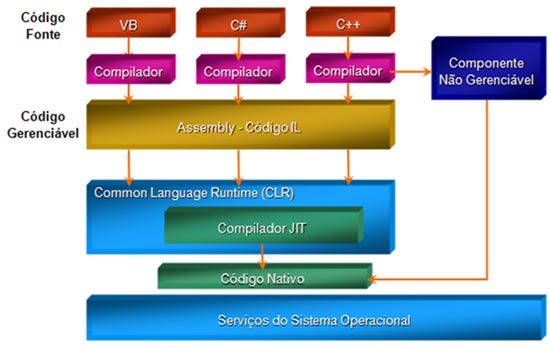
\includegraphics[scale=0.5]{Figures/ProcessoCompilacaoCLR}
		\caption{Processo de Compilação utilizando CLR}
	\end{figure}
	
	\newpage
	Algumas características da CLR são:
	
	\begin{itemize}
	\item Garbage Collector
	\item Facilidade para utilizar componentes desenvolvidos em outras linguagens
	
	\end{itemize}
	
	\subsection{CIL}
	
	A Common Intermediate Language (CIL), anteriormente chamada de Microsoft Intermediate Language (MSIL), é uma linguagem de programação de baixo nível definida pela Common Language Infrastructure (CLI), que é utilizada pelo Framework .NET e Mono.

	\subsection{Mono}
	
	Mono é uma plataforma de desenvolvimento Open Source baseada no framework .NET que permite o desenvolvimento de aplicações multiplataforma. A implementação do Mono é segue os padrões ECMA para C\# e Common Language Infrastructure(CLI).
	
	Como neste projeto o sistema operacional utilizado é o Ubuntu 16.04 e o framework .NET é uma ferramenta exclusiva da Microsoft, iremos utilizar o Mono.
	
	\subsubsection{Instalação Mono}
	
	\begin{figure}[h!]
		\centering
		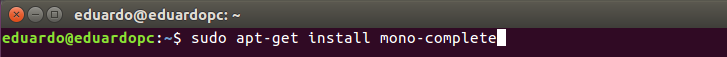
\includegraphics[scale=0.5]{Figures/Instalarmono}
		\caption{Instalando Mono no Ubuntu}
	\end{figure}
	
	\subsubsection{Compilando no Mono}
	
	\begin{figure}[h!]
	\centering
	
\includegraphics[scale=0.5]{Figures/compilarmono}
	\caption{Compilando Mono no Ubuntu}
	\end{figure}
	
	\subsubsection{Executando no Mono}
	
	\begin{figure}[h!]
	\centering
	
\includegraphics[scale=0.5]{Figures/executarmono}
	\caption{Executando Mono no Ubuntu}
	\end{figure}
	
	\subsubsection{Gerar assembly a partir de um executável no Mono}
	
	\begin{figure}[h!]
	\centering
	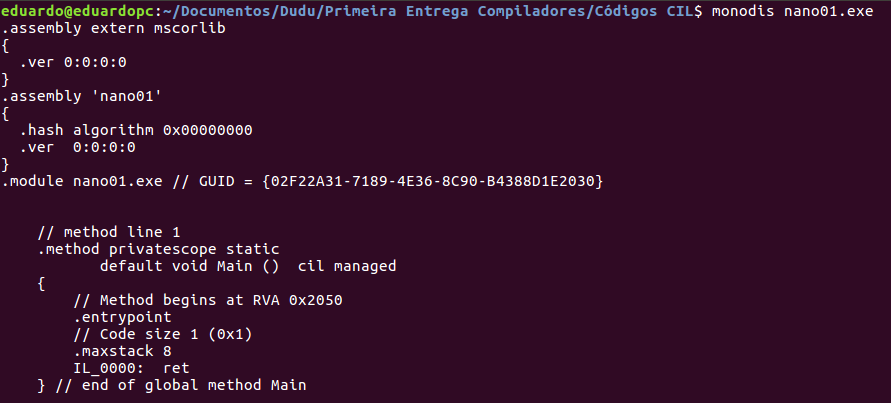
\includegraphics[scale=0.5]{Figures/exeparaassemblymono}
	\caption{Gerando assembly a partir de um executável no Mono.}
	\end{figure}
	
	\newpage
	\subsubsection{Gerar executável a partir de um assembly no Mono}
	\begin{figure}[h!]
	\centering
	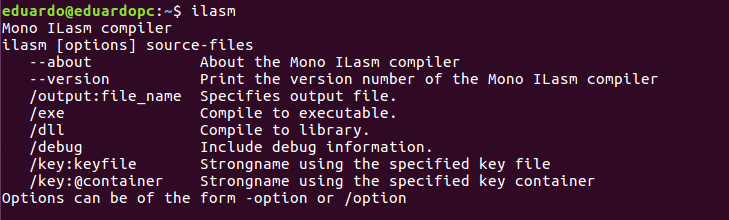
\includegraphics[scale=0.5]{Figures/ilasm}
	\caption{O comando ilasm}
	\end{figure}
	
	\begin{figure}[h!]
	\centering
	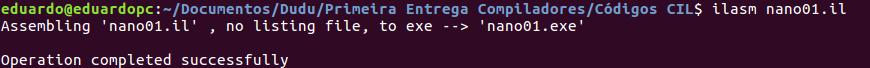
\includegraphics[scale=0.5]{Figures/ilasmmono}
	\caption{Gerando executável a partir de um assembly .il no Mono}
	\end{figure}	
	
	\newpage
	\subsection{Portugol}
	
	Portugol é uma linguagem de programação totalmente em português, muito usada para ensinar iniciantes em computação. Por ser uma linguagem com comandos em português o aluno não necessita de saber o inglês para programar, dessa forma o aluno foca na lógica de programação e não se perde nos comandos. 
	
\section{Códigos}	

\subsection{Exemplo de codigo em C \# e seu equivalente em assembly}

\begin{lstlisting}[caption=Atribuição de duas operações aritméticas sobre inteiros a uma variável(C\#)]
using System;

class nano09{

public static void Main()
{
	int n;
	n = 1+1/2;
	if(n==1)
	{
	   Console.WriteLine(n);
	}
	else
	{
	   Console.WriteLine(0);
	}

	
}

}

\end{lstlisting}


\begin{lstlisting}[caption=Atribuição de duas operações aritméticas sobre inteiros a uma variável(Código em CIL gerado pelo comando monodis)]
.assembly extern mscorlib
{
  .ver 4:0:0:0
  .publickeytoken = (B7 7A 5C 56 19 34 E0 89 ) // .z\V.4..
}
.assembly 'nano09'
{
  .custom instance void class [mscorlib]System.Runtime.CompilerServices.RuntimeCompatibilityAttribute::'.ctor'() =  (
		01 00 01 00 54 02 16 57 72 61 70 4E 6F 6E 45 78   // ....T..WrapNonEx
		63 65 70 74 69 6F 6E 54 68 72 6F 77 73 01       ) // ceptionThrows.

  .hash algorithm 0x00008004
  .ver  0:0:0:0
}
.module nano09.exe // GUID = {B11A0372-0BF1-40E0-B512-30D05E235D9B}


  .class private auto ansi beforefieldinit nano09
  	extends [mscorlib]System.Object
  {

    // method line 1
    .method public hidebysig specialname rtspecialname 
           instance default void '.ctor' ()  cil managed 
    {
        // Method begins at RVA 0x2050
	// Code size 7 (0x7)
	.maxstack 8
	IL_0000:  ldarg.0 
	IL_0001:  call instance void object::'.ctor'()
	IL_0006:  ret 
    } // end of method nano09::.ctor

    // method line 2
    .method public static hidebysig 
           default void Main ()  cil managed 
    {
        // Method begins at RVA 0x2058
	.entrypoint
	// Code size 27 (0x1b)
	.maxstack 2
	.locals init (
		int32	V_0)
	IL_0000:  ldc.i4.1 
	IL_0001:  stloc.0 
	IL_0002:  ldloc.0 
	IL_0003:  ldc.i4.1 
	IL_0004:  bne.un IL_0014

	IL_0009:  ldloc.0 
	IL_000a:  call void class [mscorlib]System.Console::WriteLine(int32)
	IL_000f:  br IL_001a

	IL_0014:  ldc.i4.0 
	IL_0015:  call void class [mscorlib]System.Console::WriteLine(int32)
	IL_001a:  ret 
    } // end of method nano09::Main

  } // end of class nano09



\end{lstlisting}


\subsection{Nano 01}
	
	\begin{lstlisting}[caption=Módulo mínimo que caracteriza um programa (Portugol)]
algoritmo "nano01"
var
inicio
fim_algoritmo
	\end{lstlisting}

\begin{lstlisting}[caption=Módulo mínimo que caracteriza um programa (CIL)]	
.assembly extern mscorlib {}
.assembly nano01 {}

.method static void Main() cil managed
{
  .entrypoint
  ret
}
\end{lstlisting}
	
	
	
	Podemos notar que o código em CIL inicia chamando a biblioteca mscorlib ({\bf M}icro{\bf s}oft {\bf C}ommon {\bf O}bject {\bf R}untime). Essa biblioteca é a principal biblioteca ao utilizar o framework .NET.
	O comando .entrypoint marca o início do programa e o comando ret marca o fim.
	
	
	
\subsection{Nano 02}
	
	\begin{lstlisting}[caption=Declaração de uma variável (Portugol)]
algoritmo "nano02"
var
  n: inteiro
inicio
fim_algoritmo
	\end{lstlisting}

\begin{lstlisting}[caption=Declaração de uma variável (CIL)]	
.assembly extern mscorlib {}
.assembly nano02 {}

.method static void Main() cil managed
{
  .entrypoint
  .maxstack 1
  .locals init ( int32 )
  ret
}
\end{lstlisting}

\subsection{Nano 03}

	\begin{lstlisting}[caption=Atribuição de um inteiro a uma variável (Portugol)]
algoritmo "nano03"
var
  n: inteiro
inicio
  n <- 1
fim_algoritmo
	\end{lstlisting}
	
	\begin{lstlisting}[caption=Atribuição de um inteiro a uma variável (CIL)]
.assembly extern mscorlib {}
.assembly nano03 {}

.method static void Main() cil managed
{
  .entrypoint
  .maxstack 1
  .locals init ( int32 )
  ldc.i4 1 
  stloc.0
  ret
}
	\end{lstlisting}

	O comando {\bf ldc.i4} coloca o número 1 do tipo {\bf int32} na pilha.
	O comando {\bf stloc.0} tira da pilha e guarda na variável local 0.
\subsection{Nano 04}

\begin{lstlisting}[caption=Atribuição de uma soma de inteiros a uma variável (Portugol)]
algoritmo "nano04"
var
  n: inteiro
inicio
  n <- 1 + 2
fim_algoritmo

\end{lstlisting}
\begin{lstlisting}[caption=Atribuição de uma soma de inteiros a uma variável (CIL)]
.assembly extern mscorlib {}
.assembly nano04 {}

.method static void Main() cil managed
{
  .entrypoint
  .maxstack 3
  .locals init (int32, int32, int32)
  ldc.i4 1
  stloc.0
  ldc.i4 2
  stloc.1
  
  ldloc.0
  ldloc.1
  add
  stloc.2

  ret
}

\end{lstlisting}

O comando {\bf ldloc} carrega uma determinada variável local na pilha. O comando {\bf add} retira as duas variáveis da pilha, executa a soma e retorna o resultado para a pilha. O comando {\bf stloc.2} carrega o resultado na variável local 2.

\subsection{Nano 05}

\begin{lstlisting}[caption=Inclusão do comando de impressão (Portugol)]
algoritmo "nano05"
var
  n : inteiro
inicio
  n <- 2
  escreva(n)
fim_algoritmo

\end{lstlisting}

\begin{lstlisting}[caption=Inclusão do comando de impressão (CIL)]
.assembly extern mscorlib {}
.assembly nano05 {}

.method static void Main() cil managed
{
  .entrypoint
  .maxstack 1
  .locals init (int32)
  ldc.i4 2
 
  call void [mscorlib]System.Console::WriteLine(int32)

  ret
}

\end{lstlisting}

\subsection{Nano 06}

\begin{lstlisting}[caption=Atribuição de uma subtração de inteiros a uma variável (Portugol)]
algoritmo "nano06"
var
  n : inteiro
inicio
  n <- 1 - 2
  escreva(n)
fim_algoritmo

\end{lstlisting}

\begin{lstlisting}[caption=Atribuição de uma subtração de inteiros a uma variável (CIL)]
.assembly extern mscorlib {}
.assembly nano06 {}

.method static void Main() cil managed
{
  .entrypoint
  .maxstack 3
  .locals init (int32, int32, int32)
  ldc.i4 1
  stloc.0
  ldc.i4 2
  stloc.1
  
  ldloc.0
  ldloc.1
  sub
  stloc.2

  ldloc.2
  call void [mscorlib]System.Console::WriteLine(int32)

  ret
}
\end{lstlisting}
\subsection{Nano 07}
\begin{lstlisting}[caption=Inclusão do comando condicional (Portugol)]
algoritmo "nano07"
var
  n : inteiro
inocio
  n <- 1
  se n = 1 entao
    escreva(n)
  fim_se
fim_algoritmo

\end{lstlisting}

\begin{lstlisting}[caption=Inclusão de comando condicional (CIL)]
.assembly extern mscorlib {}
.assembly nano07 {}

.method static void Main() cil managed
{
  .entrypoint
  .maxstack 2
  .locals init (int32, int32)
  ldc.i4 1
  stloc.0
  ldc.i4 1
  stloc.1
  ldloc.0
  ldloc.1
  beq IGUAL
  br NAOIGUAL
  IGUAL:
   ldloc.0	
   call void [mscorlib]System.Console::WriteLine(int32)
  NAOIGUAL:
  	ret
}
\end{lstlisting}

\subsection{Nano 08}

\begin{lstlisting}[caption=Inclusão do comando condicional com parte senão(Portugol)]
algoritmo "nano08"
var
  n : inteiro
inicio
  n <- 1
  se n = 1 entao
    escreva(n)
  senao
    escreva(0)
  fim_se
fim_algoritmo
\end{lstlisting}

\begin{lstlisting}[caption=Inclusão do comando condicional com parte senão(CIL)]
.assembly extern mscorlib {}
.assembly nano08 {}

.method static void Main() cil managed
{
  .entrypoint
  .maxstack 2
  .locals init (int32, int32)
  ldc.i4 1
  stloc.0
  ldloc.0

  ldc.i4 1
  beq IGUAL
  br NAOIGUAL
  IGUAL:
   ldloc.0
   call void [mscorlib]System.Console::WriteLine(int32)
   br FIM
  NAOIGUAL:
   ldc.i4 0
   call void [mscorlib]System.Console::WriteLine(int32)
  FIM:  
   ret
}
\end{lstlisting}


O programa acima funciona da seguinte maneira: Inicialmente usamos o comando {\bf ldc} para colocar o número 1 na pilha e guardamos na variável local 0, {\bf stloc.0}, para representar nossa variável {\bf n}. Após isso carregamos essa variável na pilha e colocamos o valor 1 também nesta pilha para fazermos uma comparação com o comando {\bf beq} (branch if equal). Se esses dois valores forem iguais printamos o que está em {\bf ldloc.0}, que é nossa variável n. Se não forem iguais printamos o valor 0, pois colocamos esse valor na pilha com o comando {\bf ldc.i4 0}.



\subsection{Nano 09}
\begin{lstlisting}[caption=Atribuição de duas operações aritméticas sobre inteiros a uma variável(Portugol)]
algoritmo "nano09"
var
  n : inteiro
inicio
  n <- 1 + 1 / 2
  se n = 1 entao
    escreva(n)
  senao
    escreva(0)
  fim_se
fim_algoritmo
\end{lstlisting}

\begin{lstlisting}[caption=Atribuição de duas operações aritméticas sobre inteiros a uma variável(CIL)]

.assembly extern mscorlib {}
.assembly nano09 {}

.method static void Main() cil managed
{
  .entrypoint
  .maxstack 2
  .locals init (float32, float32)
  ldc.r4 1
  ldc.r4 2
  div
  ldc.r4 1
  add
  
  stloc.0
  ldloc.0

  ldc.r4 1
  beq IGUAL
  br NAOIGUAL
  IGUAL:
   ldloc.0
   call void [mscorlib]System.Console::WriteLine(float32)
   br FIM
  NAOIGUAL:
   ldc.r4 0
   call void [mscorlib]System.Console::WriteLine(float32)
  FIM:  
    ret
}

\end{lstlisting}



\subsection{Nano 10}

\begin{lstlisting}[caption=Atribuição de variáveis inteiras(Portugol)]
algoritmo "nano10"
var
   n, m : inteiro
inicio
   n <- 1
   m <- 2
   se n = m entao
     escreva(n)
   senao
     escreva(0)
   fim_se
fim_algoritmo
\end{lstlisting}

\begin{lstlisting}[caption=Atribuição de variáveis inteiras(CIL)]
.assembly extern mscorlib {}
.assembly nano10 {}

.method static void Main() cil managed
{
  .entrypoint
  .maxstack 2
  .locals init (int32, int32)
  ldc.i4 1
  stloc.0
  ldc.i4 2
  stloc.1
  ldloc.0
  ldloc.1
  
  beq IGUAL
   ldc.i4 0
   call void [mscorlib]System.Console::WriteLine(int32)
   br FIM	
  IGUAL:
   ldloc 0
   call void [mscorlib]System.Console::WriteLine(int32)
  FIM:  
   ret

}
\end{lstlisting}

\subsection{Nano 11}
\begin{lstlisting}[caption=Introdução do comando de repetição enquanto(Portugol)]
algoritmo "nano11"
var
  n, m, x : inteiro
inicio
  n <- 1
  m <- 2
  x <- 5
  enquanto x > n faca
    n <- n + m
    escreva(n)
  fim_enquanto
fim_algoritmo
\end{lstlisting}

\begin{lstlisting}[caption=Introdução do comando de repetição enquanto(CIL)]
.assembly extern mscorlib {}
.assembly nano11 {}

.method static void Main() cil managed
{
  .entrypoint
  .maxstack 3
  .locals init (int32,int32,int32)
   ldc.i4 1  //n
   stloc.0
   ldc.i4 2  //m
   stloc.1
   ldc.i4 5  //x
   stloc.2
   LOOP:
     ldloc.2
     ldloc.0
     ble FIM
     
     ldloc.0
     ldloc.1
     add
     stloc.0
     ldloc.0
     call void [mscorlib]System.Console::WriteLine (int32)
     br LOOP
   FIM:
     ret
}
\end{lstlisting}
\subsection{Nano 12}
\begin{lstlisting}[caption=Comando condicional aninhando em um comando de repetição(Portugol)]
algoritmo "nano12"
var
   n, m, x : inteiro
inicio
   n <- 1
   m <- 2
   x <- 5
   enquanto x > n faca
     se n = m entao
     escreva(n)
   senao
     escreva(0)
   fim_se
   x <- x - 1
fim_enquanto
\end{lstlisting}

\begin{lstlisting}[caption=Comando condicional aninhando em um comando de repetição(CIL)]
.assembly extern mscorlib {}
.assembly nano12 {}

.method static void Main() cil managed
{
  .entrypoint
  .maxstack 3
  .locals init (int32,int32,int32)
  ldc.i4 1
  stloc.0
  ldc.i4 2
  stloc.1
  ldc.i4 5
  stloc.2
  LOOP:
   ldloc.2
   ldloc.0
   ble FIM
   
   ldloc.0
   ldloc.1
   beq SE_N_IGUAL_M
     ldc.i4 0
     call void [mscorlib]System.Console::WriteLine (int32)
     br DECREMENTAR_X

   SE_N_IGUAL_M:
     ldloc.0
     call void [mscorlib]System.Console::WriteLine (int32)
     br DECREMENTAR_X
   
   DECREMENTAR_X:
     ldloc.2
     ldc.i4 1
     sub
     stloc.2
     br LOOP
   FIM:
     ret
}
\end{lstlisting}

\subsection{Micro 01}

\begin{lstlisting}[caption=Converte graus Celsius para Fahrenheit(Portugol)]
algoritmo "micro01"
/*
Funcao: Ler uma temperatura em graus Celsius e apresenta-la
convertida em graus Fahrenheit. A formula de conversao e:
F=(9*C+160) / 5,
sendo F a temperatura em Fahrenheit e C a temperatura em
Celsius.
*/
var
  cel, far: real
inicio
  escreval("Tabela de conversao: Celsius -> Fahrenheit")
  escreva("Digite a temperatura em Celsius: ")
  leia(cel)
  far <- (9*cel+160)/5
  escreval("A nova temperatura e: ",far," F")
fim_algoritmo
\end{lstlisting}

\begin{lstlisting}[caption=Converte graus Celsius para Fahrenheit(CIL)]
.assembly extern mscorlib {}
.assembly micro01 {}

.method static void Main() cil managed
{

  .entrypoint
  .maxstack 10
  .locals init (float32,float32)
  
  ldstr "Tabela de Conversao: Celsius -> Fahrenheit."
  call void [mscorlib]System.Console::WriteLine (string)
  ldstr "Escreva a temperatura em Celsius: "
  call void [mscorlib]System.Console::WriteLine (string)
  call string [mscorlib]System.Console::ReadLine ()
  call float32 [mscorlib]System.Single::Parse(string)
  stloc.0
  ldloc.0
  ldc.r4 9
  mul
  ldc.r4 160
  add
  ldc.r4 5
  div
  stloc.1
  ldstr "A nova temperatura eh: "
  call void [mscorlib]System.Console::WriteLine (string)
  ldloc.1
  call void [mscorlib]System.Console::WriteLine (float32)
  ret
}
\end{lstlisting}

\subsection{Micro 02}


\begin{lstlisting}[caption=Ler dois inteiros e decide qual é maior(Portugol)]
algoritmo "micro02"

var
  num1, num2: inteiro
inicio
  escreva("Digite o primeiro numero: ")
  leia(num1)
  escreva("Digite o segundo numero: ")
  leia(num2)
  se num1 > num2 entao
    escreva("O primeiro numero ",num1," e maior que o segundo",num2)
  senao
    escreva("O segundo numero",num2," e maior que o primeiro",num1)
fim_se
fim_algoritmo
\end{lstlisting}

\begin{lstlisting}[caption=Ler dois inteiros e decide qual é maior(CIL)]
.assembly extern mscorlib {}
.assembly micro02 {}

.method static void Main() cil managed
{
  .entrypoint
  .maxstack 2
  .locals init (int32,int32)
  ldstr "Escreva o primeiro numero: "
  call void [mscorlib]System.Console::WriteLine (string)
  call string [mscorlib]System.Console::ReadLine ()
  call int32 [mscorlib]System.Int32::Parse(string)
  stloc.0
  ldstr "Escreva o segundo numero: " 
  call void [mscorlib]System.Console::WriteLine (string)
  call string [mscorlib]System.Console::ReadLine ()
  call int32 [mscorlib]System.Int32::Parse(string)
  stloc.1
  ldloc.0
  ldloc.1
  bgt PRIMEIROMAIORSEGUNDO
    ldstr "Segundo numero eh maior que o primeiro!"
    call void [mscorlib]System.Console::WriteLine (string)
    ldstr "Primeiro numero: "
    call void [mscorlib]System.Console::WriteLine (string)
    ldloc.0
    call void [mscorlib]System.Console::WriteLine (int32)
    ldstr "Segundo numero: "
    call void [mscorlib]System.Console::WriteLine (string)
    ldloc.1
    call void [mscorlib]System.Console::WriteLine (int32)
    br FIM
  PRIMEIROMAIORSEGUNDO:
    ldstr "Primeiro numero eh maior que o segundo!"
    call void [mscorlib]System.Console::WriteLine (string)
    ldstr "Primeiro numero: "
    call void [mscorlib]System.Console::WriteLine (string)
    ldloc.0
    call void [mscorlib]System.Console::WriteLine (int32)
    ldstr "Segundo numero: "
    call void [mscorlib]System.Console::WriteLine (string)
    ldloc.1
    call void [mscorlib]System.Console::WriteLine (int32)
    FIM:
     ret
}
\end{lstlisting}

\subsection{Micro 03}

\begin{lstlisting}[caption=Lê um número e verifica se ele está entre 100 e 200(Portugol)]
algoritmo "micro03"

var
  numero: inteiro
inicio
  escreva("Digite um numero: ")
  leia(numero)
  se numero >= 100 entao
    se numero <= 200 entao
      escreval("O numero esta no intervalo entre 100 e 200")
    senao
      escreval("O numero nao esta no intervalo entre 100 e 200")
    fim_se
  senao 
    escreval("O numero nao esta no intervalo entre 100 e 200")
fim_se
fim_algoritmo
\end{lstlisting}

\begin{lstlisting}[caption=Lê um número e verifica se ele está entre 100 e 200(CIL)]
.assembly extern mscorlib{}
.assembly micro03 {}

.method static void Main() cil managed
{
  .entrypoint
  .maxstack 3
  .locals init (int32)
  ldstr "Escreva um numero: "
  call void [mscorlib]System.Console::WriteLine (string)
  call string [mscorlib]System.Console::ReadLine ()
  call int32 [mscorlib]System.Int32::Parse(string)
  stloc.0
  ldloc.0
  ldc.i4 100
  bge MAIORIGUALACEM
  br FORAINTERVALO
  MAIORIGUALACEM:
   ldloc.0
   ldc.i4 200
  ble DENTROINTERVALO
  br FORAINTERVALO
  DENTROINTERVALO:
   ldstr "O numero esta no intervalo entre 100 e 200"
   call void [mscorlib]System.Console::WriteLine (string)
   br FIM
  FORAINTERVALO:
   ldstr "O numero nao esta no intervalo entre 100 e 200"
   call void [mscorlib]System.Console::WriteLine (string)
   br FIM
  FIM:
   ret
}
\end{lstlisting}

\subsection{Micro 04}

\begin{lstlisting}[caption=Lê números e informa quais estão entre 10 e 150(Portugol)]
algoritmo "micro04"

var
  x, num, intervalo: inteiro
inicio
  para x de 1 ate 5 faca
    escreva("Digite um numero: ")
    leia(num)
    se num >= 10 entao
      se num <= 150 entao
        intervalo <- intervalo + 1
      fim_se
    fim_se
  fim_para
  escreval("Ao total, foram digitados ",intervalo," numeros no
intervalo entre 10 e 150")
fim_algoritmo
\end{lstlisting}

\begin{lstlisting}[caption=Lê números e informa quais estão entre 10 e 150(CIL)]
.assembly extern mscorlib{}
.assembly micro04 {}

.method static void Main() cil managed
{
  .entrypoint
  .maxstack 5
  .locals init (int32,int32,int32)
  ldc.i4 0
  stloc.2 //intervalo
  ldc.i4 1
  stloc.0 //variavel pro loop que comeca com x=1
  COMECALOOP:
   ldloc.0 //x
   ldc.i4.5
   bgt ESCREVEQUANTIDADE
   ldstr "Digite um numero: "
   call void [mscorlib]System.Console::WriteLine (string)
   call string [mscorlib]System.Console::ReadLine ()
   call int32 [mscorlib]System.Int32::Parse(string)
   stloc.1 //num 
   ldloc.0 //x
   ldc.i4.1
   add
   stloc.0
   ldloc.1  //num
   ldc.i4 10
   bge MAIORQUE10 
   br COMECALOOP
   
   MAIORQUE10:
    ldloc.1 //num
    ldc.i4 150
    ble MENORQUE150
    br COMECALOOP
    
   MENORQUE150:
     ldloc.2 //intervalo
     ldc.i4.1
     add
     stloc.2
     br COMECALOOP
    
   ESCREVEQUANTIDADE:
     ldstr "Quantidade de numeros digitados no intervalo entre 10 e 150: "
     call void [mscorlib]System.Console::WriteLine (string)
     ldloc.2
     call void [mscorlib]System.Console::WriteLine (int32)
     br FIM
   FIM:
     ret
}
\end{lstlisting}

\subsection{Micro 05}

\begin{lstlisting}[caption=Lê strings e caracteres(Portugol)]
algoritmo "micro05"

var
  nome, sexo: caractere
  x, h, m: inteiro
inicio
  para x de 1 ate 5 faca
    escreva("Digite o nome: ")
    leia(nome)
    escreva("H - Homem ou M - Mulher: ")
    leia(sexo)
    escolha sexo
    	caso 'H'
      		h <- h + 1
    	caso 'M'
      		m <- m + 1
    	outrocaso
      		escreval("Sexo so pode ser H ou M!")
    fim_escolha
  fim_para
  escreval("Foram inseridos",h," Homens")
  escreval("Foram inseridos",m," Mulheres")
fim_algoritmo
\end{lstlisting}

\begin{lstlisting}[caption=Lê strings e caracteres(CIL)]
.assembly extern mscorlib{}
.assembly micro05{}

.method static void Main() cil managed
{
  .entrypoint
  .maxstack 10
  .locals init (int32 x,int32 h,int32 m,char sexo,string nome)
  ldc.i4.1
  stloc.0 //x
  ldc.i4.0
  stloc.1  //h
  ldc.i4.0
  stloc.2  //m
  
  LOOP:
    ldloc.0
    ldc.i4.5
    bgt IMPRIME
    ldstr "Digite o nome: "
    call void [mscorlib]System.Console::WriteLine (string)
    call string [mscorlib]System.Console::ReadLine ()
    stloc nome  //nome
    ldstr "H - Homem ou M - Mulher: "
    call void [mscorlib]System.Console::WriteLine (string)
    call string [mscorlib]System.Console::ReadLine ()
    call char [mscorlib]System.Char::Parse(string)
    stloc sexo
    ldloc sexo
    ldc.i4 72
    bne.un VERIFMULHER
    ldloc.1  //h
    ldc.i4.1
    add
    stloc.1  //h
    br INCRX
    

INCRX:
     ldloc.0 //x
     ldc.i4.1
     add
     stloc.0
     br LOOP

VERIFMULHER:
   ldloc sexo
   ldc.i4 77
   bne.un OUTROCASO
   ldloc.2 //m
   ldc.i4.1
   add
   stloc.2 //m
   br INCRX

OUTROCASO:
   ldstr "Sexo so pode ser H ou M!"
   call void [mscorlib]System.Console::WriteLine (string)
   br LOOP

IMPRIME:
  ldstr "Foram inseridos "
  call void [mscorlib]System.Console::Write(string)
  ldloc.1 //h
  call void [mscorlib]System.Console::Write(int32)
  ldstr " homens"
  call void [mscorlib]System.Console::WriteLine (string)  
  ldstr "Foram inseridas "
  call void [mscorlib]System.Console::Write(string)
  ldloc.2 //m
  call void [mscorlib]System.Console::Write(int32)
  ldstr " mulheres"
  call void [mscorlib]System.Console::WriteLine(string)
 
FIM:
  ret
}
\end{lstlisting}

\subsection{Micro 06}

\begin{lstlisting}[caption=Escreve um número lido por extenso(Portugol)]
algoritmo "micro06"

var
  numero: inteiro
inicio
  escreva("Digite um numero de 1 a 5: ")
  leia(numero)
  escolha numero
  caso 1
    escreval("Um")
  caso 2
    escreval("Dois")
  caso 3
    escreval("Tres")
  caso 4
    escreval("Quatro")
  caso 5
    escreval("Cinco")
  outrocaso
    escreval("Numero Invalido!!!")
  fim_escolha
fim_algoritmo
\end{lstlisting}

\begin{lstlisting}[caption=Escreve um número lido por extenso(CIL)]
.assembly extern mscorlib{}
.assembly micro06 {}

.method static void Main() cil managed
{
  .entrypoint
  .maxstack 3
  .locals init (int32 numero)
  ldstr "Digite um numero de 1 a 5: "
  call void [mscorlib]System.Console::WriteLine (string)
  call string [mscorlib]System.Console::ReadLine ()
  call int32 [mscorlib]System.Int32::Parse(string)
  stloc numero
  ldloc numero
  ldc.i4.1 
  bne.un DOIS //Comparo se 1 e igual ao numero digitado, se nao for ramifica pq "bne"
  ldstr "Um" //Se for entao printa 1
  call void [mscorlib]System.Console::WriteLine (string)
  br FIM
  
  DOIS:
   ldloc numero 
   ldc.i4.2   
   bne.un TRES  //Comparo se 2 e igual ao numero digitado, se nao for ramifica pq "bne"
   ldstr "Dois" //Se for entao printa 2 e assim por diante...
   call void [mscorlib]System.Console::WriteLine (string)
   br FIM

  TRES:
   ldloc numero
   ldc.i4.3
   bne.un QUATRO
   ldstr "Tres"
   call void [mscorlib]System.Console::WriteLine (string)
   br FIM

  QUATRO:
   ldloc numero
   ldc.i4 4
   bne.un CINCO
   ldstr "Quatro"
   call void [mscorlib]System.Console::WriteLine (string)
   br FIM

  CINCO:
   ldloc numero
   ldc.i4 5
   bne.un OUTROCASO
   ldstr "Cinco"
   call void [mscorlib]System.Console::WriteLine (string)
   br FIM
  
  OUTROCASO:
   ldstr "Numero invalido!!!"
   call void [mscorlib]System.Console::WriteLine (string)
   br FIM

  FIM:
   ret
   
}
\end{lstlisting}


A instrução {\bf bne.un} (branch if unequal or unordered) ramifica se dois operandos são diferentes ou desordenados.
\subsection{Micro 07}

\begin{lstlisting}[caption=Decide se os números são positivos zeros ou negativos(Portugol)]
algoritmo "micro07"

var
  programa, numero: inteiro
  opc: caractere
inicio
  programa <- 1
  enquanto programa = 1 faca
    escreva("Digite um numero: ")
    leia(numero)
    se numero > 0 entao
      escreval("Positivo")
    senao
      se numero = 0 entao
        escreval("O numero e igual a 0")
      fim_se
      se numero < 0 entao
        escreval("Negativo")
      fim_se
    fim_se
   escreva("Deseja finalizar? (S/N) ")
   leia(opc)
   se opc = "S" entao
     programa <- 0
   fim_se
  fim_enquanto
fim_algoritmo
\end{lstlisting}

\begin{lstlisting}[caption=Decide se os números são positivos zeros ou negativos(CIL)]
.assembly extern mscorlib{}
.assembly micro10 {}

.method static void Main() cil managed
{
  .entrypoint
  .maxstack 10
  .locals init (int32 numero, int32 fat)
  ldstr "Digite um numero: "
  call void [mscorlib]System.Console::WriteLine (string)
  call string [mscorlib]System.Console::ReadLine ()
  call int32 [mscorlib]System.Int32::Parse(string)
  stloc numero
  ldloc numero
  call int32 fatorial(int32)
  stloc fat //guardo em fat o retorno da funcao
  ldloc fat
  call void [mscorlib]System.Console::WriteLine (int32)
  
  ret
}

.method public static int32 fatorial(int32 n) cil managed
{
  .maxstack 10
  ldarg n //Carrega o argumento da funcao na pilha
  ldc.i4.0
  ble RET1 //branch if less than or equal to
  ldarg n 
  ldc.i4.1 
  sub
  call int32 fatorial(int32)
  ldarg n
  mul
  br FIM

 RET1:
  ldc.i4.1
  br FIM
 
 FIM:
  ret
}
\end{lstlisting}

\subsection{Micro 08}
\begin{lstlisting}[caption=Decide se um número é maior ou menor que 10(Portugol)]
algoritmo "micro08"

var
  numero: inteiro
inicio
  numero <- 1
  enquanto numero <> 0 faca
    escreva("Digite um numero: ")
    leia(numero)
    se (numero > 10) entao
      escreval("O numero ",numero," e maior que 10")
    senao
      escreval("O numero ",numero," e menor que 10")
    fim_se
  fim_enquanto
fim_algoritmo
\end{lstlisting}

\begin{lstlisting}[caption=Decide se um número é maior ou menor que 10(CIL)]
.assembly extern mscorlib{}
.assembly micro08 {}

.method static void Main() cil managed
{
  .entrypoint
  .maxstack 2
  .locals init (int32 numero)
  ldc.i4.1
  stloc numero
  LOOP:
   ldloc numero
   ldc.i4.0
   beq FIM
   ldstr "Digite um numero: "
   call void [mscorlib]System.Console::WriteLine (string)
   call string [mscorlib]System.Console::ReadLine ()
   call int32 [mscorlib]System.Int32::Parse(string)
   stloc numero
   ldloc numero
   ldc.i4 10
   bgt MAIORQUE10 //verifica se e maior que 10
   ldstr "O numero eh menor do que 10."
   call void [mscorlib]System.Console::WriteLine (string)
   br LOOP

 MAIORQUE10: 
   ldstr "O numero eh maior do que 10."
   call void [mscorlib]System.Console::WriteLine (string)
   br LOOP
 FIM:
   ret
}
\end{lstlisting}

\subsection{Micro 09}
\begin{lstlisting}[caption=Cálculo de preços(Portugol)]
algoritmo "micro09"
var
  preco, venda, novo_preco: real
inicio
  escreva("Digite o preco: ")
  leia(preco)
  escreva("Digite a venda: ")
  leia(venda)
  se (venda < 500) OU (preco < 30)
     entao novo_preco <- preco + 10/100 * preco
    senao se (vendas >= 500 E venda < 1200) OU
    (preco >= 30 E preco < 80)
        entao novo_preco <- preco + 15/100 * preco
        senao se venda >= 1200 OU preco >= 80
           entao novo_preco <- preco - 20/100 * preco
        fim_se 
    fim_se
  fim_se
  escreval("O novo preco e ", novo_preco)
fim_algoritmo
\end{lstlisting}

\begin{lstlisting}[caption=Cálculo de preços(CIL)]
.assembly extern mscorlib{}
.assembly micro09 {}

.method static void Main() cil managed
{
  .entrypoint
  .maxstack 3
  .locals init (float32 preco,float32 venda, float32 novo_preco)
  ldstr "Digite a preco: "
  call void [mscorlib]System.Console::WriteLine (string)
  call string [mscorlib]System.Console::ReadLine ()
  call float32 [mscorlib]System.Single::Parse(string)
  stloc preco
  ldstr "Digite a venda: "
  call void [mscorlib]System.Console::WriteLine (string)
  call string [mscorlib]System.Console::ReadLine ()
  call float32 [mscorlib]System.Single::Parse(string)
  stloc venda
  ldloc venda
  ldc.r4 500.0
  blt IF11
  ldloc preco
  ldc.r4 30.0
  blt IF11
  ldloc venda
  ldc.r4 500.0
  bge IF1200
  
 IF11:
  ldc.r4 1.1
  ldloc preco
  mul
  stloc novo_preco
  ldloc novo_preco
  call void [mscorlib]System.Console::WriteLine (float32)
  br FIM

 IF1200:
  ldloc venda
  ldc.r4 1200.0
  blt IF115
  br IF80

 IF80:
  ldloc preco
  ldc.r4 80.0
  blt IF115
  br IF08

 IF115:
  ldc.r4 1.15
  ldloc preco
  mul
  stloc novo_preco
  ldloc novo_preco
  call void [mscorlib]System.Console::WriteLine (float32)
  br FIM
 
 IF08:
  ldc.r4 0.8
  ldloc preco
  mul
  stloc novo_preco
  ldloc novo_preco
  call void [mscorlib]System.Console::WriteLine (float32)
  br FIM

 FIM:
  ret

}
\end{lstlisting}

\subsection{Micro 10}

\begin{lstlisting}[caption=Calcula o fatorial de um número(Portugol)]
algoritmo "micro10"

var
  numero: inteiro
  fat: inteiro
inicio
  escreva("Digite um numero: ")
  leia(numero)
  fat <- fatorial(numero)
  escreva("O fatorial de ")
  escreva(numero)
  escreva(" e ")
  escreval(fat)
fim_algoritmo

funcao fatorial(n: inteiro) : inteiro
  se n <= 0 entao
    retorne 1
  senao
    retorne n * fatorial(n-1)
  fim_funcao fatorial
\end{lstlisting}

\begin{lstlisting}[caption=Calcula o fatorial de um número(CIL)]
.assembly extern mscorlib{}
.assembly micro10 {}

.method static void Main() cil managed
{
  .entrypoint
  .maxstack 10
  .locals init (int32 numero, int32 fat)
  ldstr "Digite um numero: "
  call void [mscorlib]System.Console::WriteLine (string)
  call string [mscorlib]System.Console::ReadLine ()
  call int32 [mscorlib]System.Int32::Parse(string)
  stloc numero
  ldloc numero
  call int32 fatorial(int32)
  stloc fat //guardo em fat o retorno da funcao
  ldloc fat
  call void [mscorlib]System.Console::WriteLine (int32)
  
  ret
}

.method public static int32 fatorial(int32 n) cil managed
{
  .maxstack 10
  ldarg n //Carrega o argumento da funcao na pilha
  ldc.i4.0
  ble RET1 //branch if less than or equal to
  ldarg n 
  ldc.i4.1 
  sub
  call int32 fatorial(int32)
  ldarg n
  mul
  br FIM

 RET1:
  ldc.i4.1
  br FIM
 
 FIM:
  ret
}
\end{lstlisting}
\subsection{Micro 11}

\begin{lstlisting}[caption=Decide se um número é positivo zero ou negativo com auxílio de uma função(Portugol)]
algoritmo "micro11"

var
  numero: inteiro
  x: inteiro
inicio
  escreva("Digite um numero: ")
  leia(numero)
  x <- verifica(numero)
  se x = 1
    entao escreval("Numero positivo")
  senao se x = 0  
    entao escreval("Zero")
    senao escreval("Numero negativo")
    fim_se
  fim_se
fim_algoritmo

funcao verifica(n: inteiro) : inteiro

var
  res: inteiro
  se n > 0 entao
  res <- 1
  senao se n < 0
    entao res <- -1
    senao res <- 0
    fim_se
  fim_se
  retorne res

fim_funcao verifica
\end{lstlisting}

\begin{lstlisting}[caption=Decide se um número é positivo zero ou negativo com auxílio de uma função(CIL)]
.assembly extern mscorlib{}
.assembly micro11 {}

.method static void Main() cil managed
{
  .entrypoint
  .maxstack 3
  .locals init (int32 numero,int32 x)
  ldstr "Digite um numero: "
  call void [mscorlib]System.Console::WriteLine (string)
  call string [mscorlib]System.Console::ReadLine ()
  call int32 [mscorlib]System.Int32::Parse(string)
  
  stloc numero
  ldloc numero
  call int32 Verifica(int32)
  stloc x
  ldloc x
  ldc.i4 1
  beq POSITIVO
  ldloc x
  ldc.i4 0
  beq ZERO
  br NEGATIVO
 
 POSITIVO:
  ldstr "Numero positivo"
  call void [mscorlib]System.Console::WriteLine (string)
  br FIM

 ZERO:
  ldstr "Zero"
  call void [mscorlib]System.Console::WriteLine (string)
  br FIM
 
 NEGATIVO:
  ldstr "Numero negativo"
  call void [mscorlib]System.Console::WriteLine (string)
  br FIM

 FIM:
  ret

}

.method public static int32 Verifica(int32 n) cil managed
{
  .maxstack 4
  .locals init (int32 res)
  ldc.i4 0
  stloc res
  ldarg n
  ldc.i4.0
  bgt INCREMENTA
  ldarg n
  ldc.i4.0
  blt DECREMENTA
  ldc.i4.0
  stloc res
  br FIM
 
 INCREMENTA:
  ldloc res
  ldc.i4 1
  add
  stloc res
  br FIM
 
 DECREMENTA:
  ldloc res
  ldc.i4 1
  sub
  stloc res
  br FIM
 
 FIM:
  ldloc res
  ret

}
\end{lstlisting}

\newpage
\section{Analisador Léxico}

\subsection{Autômato Finito Determinístico}
	O analisador léxico será representado por um autômato finito determinístico, que será implementado na linguagem Ocaml. Inicialmente esse analisador reconhece a linguagem especificada pelo professor Alexsandro em sala de aula, que contém as seguintes palavras reservadas: \textit{if, then, else e print}.
	
	\begin{figure}[h!]
		\centering
		
\includegraphics[scale=0.5]{Figures/automato}
		\caption{Autômato Finito Determinístico que reconhece a linguagem definida pelo professor em sala de aula.}
	\end{figure}
	
	\newpage
	Legenda:
	
	
	\begin{itemize}
	\item Int: Estado final que reconhece números inteiros.
	\item Branco: Estado final que reconhece caracteres em branco.
	\item Op: Estado final que reconhece operadores.
	\item := : Estado final que reconhece atribuição.
	\item If: Estado final que reconhece o comando if.
	\item Then: Estado final que reconhece o comando then.
	\item Else: Estado final que reconhece o comando else.
	\item Id: Estado final que reconhece identificadores.
	\item Apar: Estado final que reconhece abertura de parenteses.
	\item Fpar: Estado final que reconhece fechamento de parenteses.
	\item Pvir: Estado final que reconhece ponto e vírgula.
	\end{itemize}
	
	Além do que foi representado no autômato, existem transições dos estados \textbf{\textit{q1,q2,q3,q4,q5,q6,q7,q8,q9,q10,q11}} para o estado \textbf{Id} que é o estado de identificador, possibilitando identificadores que possuam letras das palavras reservadas. Tal escolha foi tomada devido a dificuldade para ler o autômato caso todas essas transições fossem adicionadas. 
	
\newpage
\lstdefinestyle{OcamlStyle} {language=[Objective]Caml}
\subsection{Implementação em Ocaml}
	
	\begin{lstlisting}[style=OcamlStyle, caption=dfalexer.ml]
type estado = int
type entrada = string
type simbolo = char
type posicao = int

type dfa = {
  transicao : estado -> simbolo -> estado;
  estado: estado;
  posicao: posicao
}

type token =
 | If
 | Then
 | Else
 | Print
 | Id of string
 | Int of string
 | APar
 | FPar
 | Op of string
 | Atribuicao
 | PVir
 | Branco
 | EOF

type estado_lexico = {
   pos_inicial: posicao; (* posição inicial na string *)
   pos_final: posicao; (* posicao na string ao encontrar um estado final recente *)
   ultimo_final: estado; (* último estado final encontrado *)
   dfa : dfa;
   rotulo : estado -> entrada -> token
}

let estado_morto:estado = -1

let estado_inicial:estado = 0

let eh_letra (c:simbolo) = ('a' <= c && c <= 'z') || ('A' <= c && c <= 'Z')

let eh_digito (c:simbolo) = '0' <= c && c <= '9'

let eh_branco (c:simbolo) = c = ' ' || c = '\t' || c = '\n'

let eh_operador (c:simbolo) = c = '+' || c = '-' || c = '*' || c = '>' || c = '<' || c= '/'

let eh_estado_final e el =
  let rotulo = el.rotulo in
  try
      let _ = rotulo e "" in true
  with _ -> false

let obtem_token_e_estado (str:entrada) el =
  let inicio =  el.pos_inicial
  and fim = el.pos_final
  and estado_final = el.ultimo_final
  and rotulo = el.rotulo in
  let tamanho = fim - inicio + 1 in
  let lexema = String.sub str inicio tamanho in
  let token = rotulo estado_final lexema in
  let proximo_el = { el with pos_inicial = fim + 1;
                             pos_final = -1;
                             ultimo_final = -1;
                             dfa = { el.dfa with estado = estado_inicial;
                                                 posicao = fim + 1 }}
  in
   (token, proximo_el)


let rec analisador (str:entrada) tam el =
  let posicao_atual = el.dfa.posicao
  and estado_atual = el.dfa.estado in
  if posicao_atual >= tam
  then
    if el.ultimo_final >= 0
    then let token, proximo_el = obtem_token_e_estado str el in
      [token; EOF]
    else [EOF]
  else
    let simbolo = str.[posicao_atual]
    and transicao = el.dfa.transicao in
    let proximo_estado = transicao estado_atual simbolo in
    if proximo_estado = estado_morto
    then let token, proximo_el = obtem_token_e_estado str el in
      token :: analisador str tam proximo_el
    else
      let proximo_el =
        if eh_estado_final proximo_estado el
        then { el with pos_final = posicao_atual;
                       ultimo_final = proximo_estado;
                       dfa = { el.dfa with estado = proximo_estado;
                                           posicao = posicao_atual + 1 }}
        else { el with dfa = { el.dfa with estado = proximo_estado;
                                           posicao = posicao_atual + 1 }}
      in
      analisador str tam proximo_el

let lexico (str:entrada) =
  let trans (e:estado) (c:simbolo) =
    match (e,c) with
    | (0, 'i') -> 1 
    | (0, 't') -> 2
    | (0, 'p') -> 5
    | (0, 'e') -> 9
    | (0, ':') -> 12
    | (0, '(') -> 22
    | (0, ')') -> 23
    | (0, ';') -> 24
    | (0, _) when eh_letra c -> 21
    | (0, _) when eh_digito c -> 13
    | (0, _) when eh_branco c -> 14
    | (0, _) when eh_operador c -> 15
    | (0, _) -> failwith ("Erro lexico: caracter desconhecido " ^ Char.escaped c)
    | (1, 'f') -> 17
    | (1, _) when eh_letra c || eh_digito c -> 21
    | (2, 'h') -> 3
    | (2, _) when eh_letra c || eh_digito c -> 21
    | (3, 'e') -> 4
    | (3, _) when eh_letra c || eh_digito c -> 21
    | (4, 'n') -> 18
    | (4, _) when eh_letra c || eh_digito c -> 21
    | (5, 'r') -> 6
    | (5, _) when eh_letra c || eh_digito c -> 21
    | (6, 'i') -> 7
    | (6, _) when eh_letra c || eh_digito c -> 21
    | (7, 'n') -> 8
    | (7, _) when eh_letra c || eh_digito c -> 21
    | (8, 't') -> 19
    | (8, _) when eh_letra c || eh_digito c -> 21
    | (9, 'l') -> 10
    | (9, _) when eh_letra c || eh_digito c -> 21
    | (10, 's') -> 11
    | (10, _) when eh_letra c || eh_digito c -> 21
    | (11, 'e') -> 20 
    | (11, _) when eh_letra c || eh_digito c -> 21
    | (12, '=') -> 16
    | (13, _) when eh_digito c -> 13
    | (14, _) when eh_branco c -> 14
    | (17, _) when eh_letra c || eh_digito c -> 21
    | (18, _) when eh_letra c || eh_digito c -> 21
    | (19, _) when eh_letra c || eh_digito c -> 21
    | (20, _) when eh_letra c || eh_digito c -> 21
    | (21, _) when eh_letra c || eh_digito c -> 21
    | _ -> estado_morto
 and rotulo e str =
  match e with
  | 17 -> If
  | 1
  | 2
  | 3
  | 4
  | 5
  | 6
  | 7
  | 8
  | 9
  | 10
  | 11
  | 21 -> Id str
  | 13 -> Int str
  | 14 -> Branco
  | 15 -> Op str
  | 16 -> Atribuicao
  | 18 -> Then
  | 19 -> Print
  | 20 -> Else
  | 22 -> APar
  | 23 -> FPar
  | 24 -> PVir
  | _ -> failwith ("Erro lexico: sequencia desconhecida " ^ str)
in let dfa = { transicao = trans;
               estado = estado_inicial;
               posicao = 0 }
in let estado_lexico = {
  pos_inicial = 0;
  pos_final = -1;
  ultimo_final = -1;
  rotulo = rotulo;
  dfa = dfa
} in
  analisador str (String.length str) estado_lexico
	\end{lstlisting}
	
	Os estados do autômato que possuíam rótulos como: Int, Branco, Op, Atribuicao If, Then, Else, Id, Apar, Fpar, Pvir. Foram numerados da seguinte maneira no código em Ocaml:
	\begin{itemize}
	\item Int = 13
	\item Branco = 14
	\item Op = 15
	\item Atribuicao = 16
	\item If = 17
	\item Then = 18
	\item Print = 19
	\item Else = 20
	\item Id = 21
	\item Apar = 22
	\item Fpar = 23
	\item Pvir = 24
	\end{itemize}

\subsection{Execução}

	Para executar o código implementado em Ocaml, primeiramente utilizamos o comando \textbf{rlwrap ocaml} em um terminal Linux. Depois utilizamos o comando \textbf{\#use "nomedoarquivo.ml"}, para informar ao interpretador que utilizaremos as funções definidas neste arquivo.
	
	\begin{figure}[h!]
		\centering
		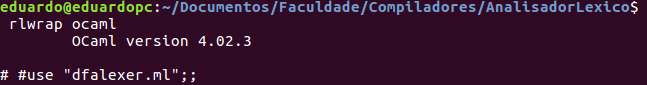
\includegraphics[scale=0.5]{Figures/rlwrap}
		\caption{Preparando ambiente para execução do analisador léxico}
	\end{figure}
	
	\begin{figure}[h!]
		\centering
		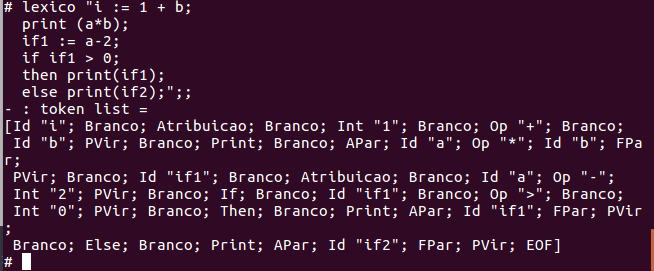
\includegraphics[scale=0.5]{Figures/Analiselexica}
		\caption{Execução do analisador léxico no programa apresentado em sala de aula}
	\end{figure}
	
	
	\subsection{Analisador Léxico para linguagem Portugol}
	
	Segue abaixo o código do arquivo \textbf{ lexico.mll} em Ocaml para o analisador léxico da linguagem Portugol. Foi utilizado o auxiliador ocamllex.
	
	\begin{lstlisting}[caption=lexico.mll, style=OcamlStyle ]
	{
  open Lexing
  open Printf

  let incr_num_linha lexbuf = 
    let pos = lexbuf.lex_curr_p in
     lexbuf.lex_curr_p <- { pos with
        pos_lnum = pos.pos_lnum + 1;
        pos_bol = pos.pos_cnum;
     }

  let msg_erro lexbuf c =
    let pos = lexbuf.lex_curr_p in
    let lin = pos.pos_lnum
    and col = pos.pos_cnum - pos.pos_bol - 1 in
    sprintf "%d-%d: caracter desconhecido %c" lin col c

type tokens = APAR
            | FPAR
            | ACOL 
            | FCOL
            | ATRIB
            | SOMA
            | SUB
            | MULT
            | DIVISAO
            | POTENCIA
            | MOD
            | IGUAL
            | MENOR
            | MENORIGUAL
            | MAIOR
            | MAIORIGUAL
            | DIFERENTE
            | NAO
            | OU
            | E
            | XOU
            | ALEATORIO
            | ALGORITMO
            | ARQUIVO
            | ASC
            | ATE
            | CARAC
            | CARACPNUM
            | CARACTER
            | CASO
            | COMPR
            | COPIA
            | CRONOMETRO
            | DE
            | DEBUG
            | DECLARA
            | ECO
            | ENQUANTO
            | ENTAO
            | ESCOLHA
            | ESCREVA
            | ESCREVAL
            | FACA
            | FALSO
            | FIMALGORITMO
            | FIMENQUANTO
            | FIMESCOLHA
            | FIMFUNCAO
            | FIMPARA
            | FIMPROCEDIMENTO
            | FIMREPITA
            | FIMSE
            | FUNCAO
            | INICIO
            | INT
            | INTEIRO
            | INTERROMPA
            | LEIA
            | LIMPATELA
            | LOGICO
            | MAIUSC
            | MINUSC
            | NUMPCARAC
            | OUTROCASO
            | PARA
            | PASSO
            | PAUSA
            | POS
            | REAL
            | PROCEDIMENTO
            | REPITA
            | RETORNE
            | SE
            | SENAO
            | TIMER
            | VAR
            | VETOR
            | VERDADEIRO
            | VIRGULA
            | LITINT of int
            | LITSTRING of string
            | LITCHAR of string 
            | ID of string
            | EOF
}

let digito = ['0' - '9']
let inteiro = digito+

let letra = ['a' - 'z' 'A' - 'Z']
let identificador = letra ( letra | digito | '_')*

let brancos = [' ' '\t']+
let novalinha = '\r' | '\n' | "\r\n"

let comentario = "//" [^ '\r' '\n' ]*


rule token = parse
  brancos    { token lexbuf }
| novalinha  { incr_num_linha lexbuf; token lexbuf }
| comentario { token lexbuf }
| "{"       { comentario_bloco 0 lexbuf }
| ','        { VIRGULA }
| '('        { APAR }
| ')'        { FPAR }
| '['        { ACOL }
| ']'        { FCOL }
| "<-"       { ATRIB }
| ':'        { DECLARA }
| '+'        { SOMA }
| '-'        { SUB }
| '*'        { MULT }
| '/'        { DIVISAO }
| '^'        { POTENCIA }
| '%'        
| "MOD"      { MOD }
| '='        { IGUAL }
| '<'        { MENOR }
| '>'        { MAIOR }
| "<="       { MENORIGUAL }
| ">="       { MAIORIGUAL }
| "<>"       { DIFERENTE }
| "nao"      { NAO }
| "ou"       { OU }
| "e"        { E }
| "xou"      { XOU }
| inteiro as num { let numero = int_of_string num in 
                    LITINT numero  } 
| "aleatorio" { ALEATORIO }
| "algoritmo" { ALGORITMO }
| "arquivo"   { ARQUIVO }
| "asc"       { ASC }
| "ate"       { ATE }
| "carac"     { CARAC }
| "caracpnum" { CARACPNUM }
| "caractere" { CARACTER }
| "caso"      { CASO }
| "compr"     { COMPR }
| "copia"     { COPIA }
| "cronometro"  { CRONOMETRO }
| "de"        { DE }
| "debug"     { DEBUG }
| "eco"       { ECO }
| "enquanto"  { ENQUANTO }
| "entao"     { ENTAO }
| "escolha"   { ESCOLHA }
| "escreva"   { ESCREVA }
| "escreval"  { ESCREVAL }
| "faca"      { FACA }
| "falso"     { FALSO }
| "fimalgoritmo" { FIMALGORITMO }
| "fimenquanto" { FIMENQUANTO }
| "fimescolha"  { FIMESCOLHA }
| "fimfuncao" { FIMFUNCAO }
| "fimpara"   { FIMPARA }
| "fimprocedimento" { FIMPROCEDIMENTO }
| "fimrepita" { FIMREPITA }
| "fimse"     { FIMSE }
| "funcao"    { FUNCAO }
| "inicio"    { INICIO }
| "int"       { INT }
| "inteiro"   { INTEIRO }
| "interrompa"  { INTERROMPA }
| "leia"      { LEIA }
| "limpatela" { LIMPATELA }
| "logico"    { LOGICO }
| "maiusc"    { MAIUSC }
| "minusc"    { MINUSC }  
| "numpcarac" { NUMPCARAC }
| "outrocaso" { OUTROCASO }
| "para"      { PARA }
| "passo"     { PASSO }
| "pausa"     { PAUSA }
| "pos"       { POS }
| "real"      { REAL }
| "procedimento"  { PROCEDIMENTO }
| "repita"    { REPITA }
| "retorne"   { RETORNE } 
| "se"        { SE }
| "senao"     { SENAO }
| "timer"     { TIMER }
| "var"       { VAR }
| "vetor"     { VETOR }
| "verdadeiro"  { VERDADEIRO }
| identificador as id { ID id }
| '''        { let buffer = Buffer.create 1 in 
               let c = leia_string buffer lexbuf in
                LITCHAR c }
| '"'        { let buffer = Buffer.create 1 in 
               let str = leia_string buffer lexbuf in
                LITSTRING str }
| _ as c  { failwith (msg_erro lexbuf c) }
| eof        { EOF }
and comentario_bloco n = parse
   "}"   { if n=0 then token lexbuf 
            else comentario_bloco (n-1) lexbuf }
| "{"    { comentario_bloco (n+1) lexbuf }
| _       { comentario_bloco n lexbuf }
| eof     { failwith "Comentário não fechado" }
and leia_string buffer = parse
   '"'    { Buffer.contents buffer}
| '''     { Buffer.contents buffer}
| "\\t"   { Buffer.add_char buffer '\t'; leia_string buffer lexbuf }
| "\\n"   { Buffer.add_char buffer '\n'; leia_string buffer lexbuf }
| '\\' '"'  { Buffer.add_char buffer '"'; leia_string buffer lexbuf }
| '\\' '\\'  { Buffer.add_char buffer '\\'; leia_string buffer lexbuf }
| _ as c    { Buffer.add_char buffer c; leia_string buffer lexbuf }
| eof     { failwith "A string não foi fechada"}


	\end{lstlisting}
	
	\begin{lstlisting}[style=OcamlStyle, caption=carregador.ml]
	
	#load "lexico.cmo";;

	let rec tokens lexbuf =
  		let tok = Lexico.token lexbuf in
  		match tok with
  		| Lexico.EOF -> [Lexico.EOF]
  		| _ -> tok :: tokens lexbuf
	;;

	let lexico str =
  		let lexbuf = Lexing.from_string str in
  		tokens lexbuf
	;;

	let lex arq =
  		let ic = open_in arq in
  		let lexbuf = Lexing.from_channel ic in
  		let toks = tokens lexbuf in
  		let _ = close_in ic in
  		toks
	\end{lstlisting}
	\subsubsection{Execução}
	
	Para executar o código deve-se seguir a seguinte ordem:
	
	\begin{enumerate}
	\item ocamllex nomedoarquivo.mll
	\item ocamlc -c nomedoarquivo.ml
	\item rlwrap ocaml
	\item \# load "nomedoarquivo.cmo" (Esse passo pode ser inserido no arquivo carregador)
	\item \# use "nomedoarquivocarregador.ml";;
	\item lex "nano01.txt";;
	\end{enumerate}

	\begin{figure}[h!]
		\centering
		\includegraphics[scale=0.5]{Figures/ocamllex}
		\caption{Procedimento para compilar e executar analisador léxico.}
	\end{figure}
	
	\newpage
	\begin{figure}[h!]
		\centering
		\includegraphics[scale=0.5]{Figures/nano01nano07}
		\caption{Tokens dos arquivos nano01 até nano07.}
	\end{figure}
	
	\newpage
	\begin{figure}[h!]
		\centering
		\includegraphics[scale=0.45]{Figures/nano08nano11}
		\caption{Tokens dos arquivos nano08 até nano11.}
	\end{figure}
	
	\newpage
	\section{Analisador sintático preditivo}
	
	Foi solicitado a entrega de um analisador sintático preditivo para a seguinte gramática:
	
	\begin{figure}[h!]
		\centering
		\includegraphics[scale=0.45]{Figures/gramaticall1}
		\caption{Gramática}
	\end{figure}
	
	\begin{figure}[h!]
		\centering
		\includegraphics[scale=0.45]{Figures/tabelall1}
		\caption{Tabela LL(1) para a gramática da figura acima}
	\end{figure}
	
	Segue abaixo os códigos em Ocaml para representar o analisador sintático para a gramática acima. Vale ressaltar que é necessário fazer o analisador léxico para a linguagem, portanto o arquivo lexico.mll deve ser alterado.
	\subsection{Códigos}	
	
	\begin{lstlisting}[caption=lexico.mll, style=OcamlStyle]
{
  open Lexing
  open Printf
  open Sintatico
         

  let incr_num_linha lexbuf = 
    let pos = lexbuf.lex_curr_p in
     lexbuf.lex_curr_p <- { pos with
        pos_lnum = pos.pos_lnum + 1;
        pos_bol = pos.pos_cnum;
     }

  let msg_erro lexbuf c =
    let pos = lexbuf.lex_curr_p in
    let lin = pos.pos_lnum
    and col = pos.pos_cnum - pos.pos_bol - 1 in
    sprintf "%d-%d: caracter desconhecido %c" lin col c


}

rule token = parse 
| 'a'        {A}
| 'b'        {B}
| 'c'        {C}
| 'd'        {D}
| 'e'        {E}
| 'f'        {F}
| _ as c  { failwith (msg_erro lexbuf c) }
| eof        { EOF }
	\end{lstlisting}
	
	\begin{lstlisting}[caption=sintatico.mli, style=OcamlStyle]
type tokens = A
            | B
            | C
            | D
            | E
            | F
            | EOF
	
	\end{lstlisting}
	
	\begin{lstlisting}[caption=sintaticoArv.ml, style=OcamlStyle]
(* Parser preditivo *)
#load "lexico.cmo";;
open Sintatico;;

type regra = S of regra * regra * regra
            | X of tokens * regra * tokens
            | Y of tokens * regra * regra * tokens * regra
            | Z of tokens * regra * regra * tokens
            | X_vazio
            | Y_d of tokens
            | Z_f of tokens

let tk = ref EOF (* variável global para o token atual *)
let lexbuf = ref (Lexing.from_string "")

(* lê o próximo token *)             
let prox () = tk := Lexico.token !lexbuf
                                 
let to_str tk =
  match tk with
    A -> "a"
  | B -> "b"
  | C -> "c"
  | D -> "d"
  | E -> "e"
  | F -> "f"
  | EOF -> "eof"

let erro esp =
  let msg = Printf.sprintf "Erro: esperava %s mas encontrei %s"
                            esp (to_str !tk)
  in
  failwith msg

let consome t = if (!tk == t) then prox() else erro (to_str t)
                                                   
let rec ntS () =
  match !tk with
    A    
   |C     
   |D     -> 
             let cmd1 = ntX() in
             let cmd2 = ntY() in
             let cmd3 = ntZ() in
             S (cmd1, cmd2, cmd3)
  | _ -> erro "a, c ou d"
and ntX () =
  match !tk with
     B
    |C
    |D
    |E
    |F    -> X_vazio 
    |A    -> let _ = consome A in 
             let cmd = ntX() in
             let _ = consome B in
             X (A, cmd, B)
    | _ -> erro "a"                               
and ntY () =
  match !tk with
    C    -> let _ = consome C in
            let cmd = ntY() in
            let cmd2 = ntZ() in
            let _ = consome C in
            let cmd3 = ntX() in
            Y (C,cmd,cmd2, C, cmd3)
   |D     -> let _ = consome D in
            Y_d (D)
   |_     -> erro "c ou d"
and ntZ () = 
  match !tk with
    E    -> let _ = consome E in
            let cmd = ntZ() in
            let cmd2 = ntY() in
            let _ = consome E in
            Z (E, cmd, cmd2, E)
   |F    -> let _ = consome F in
            Z_f (F)
   |_    -> erro "e ou f"                                           
                
let parser str =
  lexbuf := Lexing.from_string str;
  prox (); (* inicializa o token *)
  let arv = ntS () in
  match !tk with
    EOF -> let _ = Printf.printf "Ok!\n" in arv
  | _ -> erro "fim da entrada"

let teste () =
  let entrada =
      "abcdfcf"
  in
  parser entrada

	\end{lstlisting}
	
	Para a execução devemos seguir os seguintes passos:
		
	\begin{figure}[h!]
		\centering
		\includegraphics[scale=0.45]{Figures/execucaosintatico}
		\caption{Passos para a execução do analisador sintatico}
	\end{figure}
	
	Segue a execução para a palavra "abcdfcf"
	
	\begin{figure}[h!]
		\centering
		\includegraphics[scale=0.45]{Figures/testandogramatica}
		\caption{Execução para a palavra abcdfcf}
	\end{figure}
	
	
	\newpage
	\section{Analisador sintático para a linguagem Portugol}
	
	O analisador sintático para a linguagem portugol foi feito utilizando o \textbf{\textit{Menhir}}
	que é um Parser LR(1) para a linguagem de programação Ocaml.
	
	Para intalar o \textbf{\textit{Menhir}} basta seguir os passos abaixo. As mensagens durante a instação serão diferentes, pois o Menhir já estava instalado na máquina onde os testes foram realizados.	

	\subsection{Instalação Menhir}	
	\begin{figure}[h!]
		\centering
		\includegraphics[scale=0.45]{Figures/installmenhir1}
		\caption{Instalação Menhir - Parte 1}
	\end{figure}
	
	\begin{figure}[h!]
		\centering
		\includegraphics[scale=0.45]{Figures/installmenhir2}
		\caption{Instalação Menhir - Parte 2}
	\end{figure}
	
	
	\newpage
	\subsection{Códigos do Parser e da Árvore Sintática}
	\begin{lstlisting}[caption=parser.mly, style=OcamlStyle]

%{
  open Ast
%}

%token <int> INT
%token <float> FLOAT
%token <string> ID
%token <string> LITSTRING
%token <string> LITCHAR  
%token ALGORITMO
%token SOMA SUB MULT DIVISAO MOD
%token POTENCIA
%token APAR
%token FPAR
%token ACOL
%token FCOL
%token IGUAL
%token DIFERENTE
%token MAIOR
%token MAIORIGUAL
%token MENOR
%token MENORIGUAL
%token E OU NAO XOU
%token EOF
%token ATRIB
%token DECLARA 
%token PTV
%token VAR
%token INTEIRO
%token LOGICO
%token REAL
%token ATE 
%token CARACTER
%token CASO
%token DE
%token VIRGULA
%token INICIO
%token FUNCAO
%token FIMFUNCAO
%token FIMPARA 
%token FIMSE
%token FIMENQUANTO
%token FIMESCOLHA
%token SE
%token ENTAO
%token SENAO
%token ENQUANTO
%token ESCOLHA
%token ESCREVA
%token ESCREVAL
%token LEIA
%token FACA
%token OUTROCASO
%token PARA 
%token PASSO 
%token RETORNE
%token VERDADEIRO
%token FALSO
%token FIMALGORITMO


%left OU XOU
%left E
%left IGUAL DIFERENTE
%left MAIOR MAIORIGUAL MENOR MENORIGUAL
%left SOMA SUB
%left MULT DIVISAO MOD
%right POTENCIA

 


%start <Ast.prog> prog

%%
   
prog:
    | da=declaracao_algoritmo vdb=var_decl_block? fd=func_decl* stmb=stm_block  EOF { Prog (da,vdb,fd,stmb) }
    ;

declaracao_algoritmo:
    | ALGORITMO LITSTRING { DeclAlg }
    ;

var_decl_block:
    | VAR v=var_decl* { VarDeclBlock (v) }
    ;

var_decl:
    | ids = separated_nonempty_list(VIRGULA, ID) DECLARA t=tp_primitivo PTV {  List.map (fun id -> VarDecl (id,t)) ids }
    ;


tp_primitivo:
    | INTEIRO { Inteiro }
    | REAL { Real }
    | CARACTER { Caractere }
    | LOGICO { Booleano }
    ;

stm_block:
    | INICIO stms=stm_list* FIMALGORITMO { StmBlock(stms)}
    ;
stm_list:
    | stm=stm_attr {stm}
    | stm=fcall {stm}
    | stm=stm_ret {stm}
    | stm=stm_se {stm}
    | stm=stm_enquanto {stm}
    | stm=stm_para {stm}
    | stm=stm_leia {stm}
    | stm=stm_escreva {stm}
    | stm=stm_escreval {stm}
    | stm=stm_escolha {stm}
    ;

stm_ret:
    | RETORNE expr=expr? PTV { StmRetorne(expr)}
    ;

lvalue: 
    | id=ID { Var(id) }
    | lv=lvalue ACOL e=expr FCOL {VarElement(lv,e)}
    ;


stm_attr:
    | v=lvalue ATRIB e=expr PTV { StmAttrib(v,e) }
    ;

stm_se:
    | SE e=expr ENTAO stms=stm_list* senao=stm_senao? FIMSE { StmSe(e,stms,senao)}
    ;

stm_senao:
    | SENAO stm=stm_list* { StmSeNao(stm) }
    ;

stm_escolha:
    | ESCOLHA id=ID c=case+ OUTROCASO stms=stm_list* FIMESCOLHA {StmEscolha(id,c,stms) }
    ;

case:
    | CASO LITCHAR stms=stm_list* {StmCase(stms)}
    | CASO INT stms=stm_list* {StmCase(stms) }
    ;

stm_enquanto:
    | ENQUANTO expr FACA stm=stm_list* FIMENQUANTO { StmEnquanto stm }
    ;

stm_para:
    | PARA lvalue DE expr ATE expr passo? FACA stm=stm_list* FIMPARA {StmPara stm }
    ;

stm_leia:
    | LEIA APAR id=ID FPAR PTV {StmLeia id}
    ;

stm_escreva:
    | ESCREVA APAR stm=separated_nonempty_list(VIRGULA, expr) FPAR PTV {StmEscreva stm}
    ;

stm_escreval:
    | ESCREVAL APAR stm=separated_nonempty_list(VIRGULA, expr) FPAR PTV {StmEscreval stm }
    ;

passo:
    | PASSO SOMA INT { }
    | PASSO SUB INT { }
    ; 

expr:  
   | e1=expr o=op e2=expr { ExpOp(e1,o,e2) }
   | t=termo {ExpTerm t} 
   | NAO t=termo { ExpTermNeg t}
   | APAR e=expr FPAR { e }
   ;

%inline op:
  | SOMA { Soma }
  | SUB  { Subtracao }
  | MULT { Multiplicacao }
  | DIVISAO { Divisao }
  | POTENCIA { Potencia }
  | MOD { Modulo }
  | IGUAL { Igual }
  | DIFERENTE { Diferente }
  | MENOR { Menor }
  | MENORIGUAL { MenorIgual }
  | MAIOR { Maior }
  | MAIORIGUAL { MaiorIgual }
  | E { ELogico }
  | OU { OuLogico }
  | XOU { XouLogico }
  ;

termo:
  | f=fcall { TermoFcall}
  | l=literal {TermoLiteral l}
  | lv=lvalue {TermoVar lv}
  ;

literal:
  | LITSTRING { LitString}
  | i=INT { Int i}
  | f=FLOAT { Float f}
  | LITCHAR { LitChar}
  | l=logico_value { Bool l}
  ;

logico_value:
  | VERDADEIRO { Verdadeiro }
  | FALSO  { Falso }
  ;

fcall:
    | id=ID APAR args=fargs? FPAR { Fcallargs(id,args) }
    ;

fargs:
    | exprs=separated_nonempty_list(VIRGULA, expr) {  List.map (fun expr -> Fargs(expr)) exprs}
    ;

func_decl:
    | FUNCAO ID APAR fp=fparams? FPAR fy=func_type? fv=fvar_decl fb=func_bloc { FuncDecl (fp,fy,fv,fb) }
	  ;

func_type:
    | DECLARA t=tp_primitivo { FuncTipo(t) }
    ;


func_bloc:
    | INICIO stm=stm_list* FIMFUNCAO {FuncBloc(stm)}
    ;
    
fvar_decl:
    | v=var_decl_block? { FVarDecl(v) }
    ;

fparams:
    | fparam=separated_nonempty_list(VIRGULA,fparam){FParams(fparam)}
    ;

fparam:
    | id=ID DECLARA t=tp_primitivo {FParam(id,t)}
    ;


	\end{lstlisting}
	
		\begin{lstlisting}[caption=ast.ml, style=OcamlStyle]

type identificador = string

type prog = Prog of declaracao_algoritmo * var_decl_block option * func_decl_list * statements
and declaracao_algoritmo = DeclAlg
and var_decl_block = VarDeclBlock of var_decl list
and var_decl = vars list
and vars = VarDecl of identificador * tipo
and func_decl_list = func_decl list
and func_decl = FuncDecl of fparams option * functype option * fvardecl * funcbloc
and fparams = FParams of fparam list
and fparam = FParam of identificador * tipo
and functype = FuncTipo of tipo
and fvardecl = FVarDecl of var_decl_block option
and funcbloc = FuncBloc of stm_list list
and statements = StmBlock of stm_list list

and tipo = Inteiro
		  |Real
		  |Booleano
		  |Caractere

and stm_list  = StmAttrib of lvalue * expr
		  	   |Fcallargs of identificador * fargs option
		  	   |StmRetorne of expr option
		  	   |StmSe of expr * stm_list list * senao option
		  	   |StmEscolha of identificador * case list * stm_list list
		  	   |StmPara of stm_list list
		  	   |StmLeia of identificador
		  	   |StmEscreva of expr list
		  	   |StmEscreval of expr list
		  	   |StmEnquanto of stm_list list

and senao = StmSeNao of stm_list list

and case = StmCase of stm_list list

and lvalue = Var of identificador
			|VarElement of lvalue * expr

and expr = ExpOp of expr * op * expr
		  |ExpTerm of termo
		  |ExpTermNeg of termo

and op = Soma
		|Subtracao
		|Multiplicacao
		|Divisao
		|Potencia
		|Modulo
		|Igual
		|Diferente
		|Menor
		|MenorIgual
		|Maior
		|MaiorIgual
		|ELogico
		|OuLogico
		|XouLogico

and termo = TermoFcall 
		   |TermoLiteral of literal
		   |TermoVar of lvalue

and fargs = args list

and args = Fargs of expr


and literal = LitString 
			 |Int of int
			 |Float of float
			 |LitChar
			 |Bool of logico_value

and logico_value = Verdadeiro
				  |Falso
			
    


	\end{lstlisting}
	
	\newpage
	\subsection{Compilando e Executando}
	
	\begin{figure}[h!]
		\centering
		\includegraphics[scale=0.45]{Figures/processocompilacaoexecucao}
		\caption{Compilando arquivos necessários para o Parser}
	\end{figure}
	
	\begin{figure}[h!]
		\centering
		\includegraphics[scale=0.45]{Figures/parsermicro11}
		\caption{Árvore sintática para código micro11.ptg}
	\end{figure}


\clearpage
	
\section{Tratamento de Erros}

\subsection{Gerando arquivo de mensagens de erro}

Para gerar os arquivos de mensagens de erro, basta digitar o seguinte comando:

	\begin{figure}[h!]
		\centering
		\includegraphics[scale=0.5]{Figures/list-errors}
		\caption{Comando para gerar arquivo de mensagens de erro}
	\end{figure}
	
\subsection{Arquivo completo com as mensagens de erro}
\begin{lstlisting}
prog: ALGORITMO LITSTRING FUNCAO ID APAR FPAR DECLARA REAL XOU 
##
## Ends in an error in state: 33.
##
## func_decl -> FUNCAO ID APAR option(fparams) FPAR option(func_type) . fvar_decl func_bloc [ INICIO FUNCAO ]
##
## The known suffix of the stack is as follows:
## FUNCAO ID APAR option(fparams) FPAR option(func_type) 
##

<Erro: após tipo de retorno de uma função>

prog: ALGORITMO LITSTRING FUNCAO ID APAR FPAR DECLARA XOU 
##
## Ends in an error in state: 31.
##
## func_type -> DECLARA . tp_primitivo [ VAR INICIO ]
##
## The known suffix of the stack is as follows:
## DECLARA 
##

<Erro: após ":" da declaracao de uma função>

prog: ALGORITMO LITSTRING FUNCAO ID APAR FPAR INICIO FIMFUNCAO XOU 
##
## Ends in an error in state: 188.
##
## list(func_decl) -> func_decl . list(func_decl) [ INICIO ]
##
## The known suffix of the stack is as follows:
## func_decl 
##

<Erro: após fimfuncao>

prog: ALGORITMO LITSTRING FUNCAO ID APAR FPAR INICIO RETORNE PTV FIMESCOLHA 
##
## Ends in an error in state: 174.
##
## func_bloc -> INICIO list(stm_list) . FIMFUNCAO [ INICIO FUNCAO ]
##
## The known suffix of the stack is as follows:
## INICIO list(stm_list) 
##
## WARNING: This example involves spurious reductions.
## This implies that, although the LR(1) items shown above provide an
## accurate view of the past (what has been recognized so far), they
## may provide an INCOMPLETE view of the future (what was expected next).
## In state 142, spurious reduction of production list(stm_list) -> 
## In state 153, spurious reduction of production list(stm_list) -> stm_list list(stm_list) 
##

<Erro: após retorno de uma função>

prog: ALGORITMO LITSTRING FUNCAO ID APAR FPAR INICIO XOU 
##
## Ends in an error in state: 36.
##
## func_bloc -> INICIO . list(stm_list) FIMFUNCAO [ INICIO FUNCAO ]
##
## The known suffix of the stack is as follows:
## INICIO 
##

<Erro: após inicio de uma função>

prog: ALGORITMO LITSTRING FUNCAO ID APAR FPAR VAR FUNCAO 
##
## Ends in an error in state: 35.
##
## func_decl -> FUNCAO ID APAR option(fparams) FPAR option(func_type) fvar_decl . func_bloc [ INICIO FUNCAO ]
##
## The known suffix of the stack is as follows:
## FUNCAO ID APAR option(fparams) FPAR option(func_type) fvar_decl 
##
## WARNING: This example involves spurious reductions.
## This implies that, although the LR(1) items shown above provide an
## accurate view of the past (what has been recognized so far), they
## may provide an INCOMPLETE view of the future (what was expected next).
## In state 5, spurious reduction of production list(var_decl) -> 
## In state 19, spurious reduction of production var_decl_block -> VAR list(var_decl) 
## In state 20, spurious reduction of production option(var_decl_block) -> var_decl_block 
## In state 34, spurious reduction of production fvar_decl -> option(var_decl_block) 
##

<Erro: após declaração de variáveis de uma função>

prog: ALGORITMO LITSTRING FUNCAO ID APAR FPAR XOU 
##
## Ends in an error in state: 30.
##
## func_decl -> FUNCAO ID APAR option(fparams) FPAR . option(func_type) fvar_decl func_bloc [ INICIO FUNCAO ]
##
## The known suffix of the stack is as follows:
## FUNCAO ID APAR option(fparams) FPAR 
##

<Erro: após fechamento do paranteses de uma função >

prog: ALGORITMO LITSTRING FUNCAO ID APAR ID DECLARA CARACTER VIRGULA XOU 
##
## Ends in an error in state: 180.
##
## separated_nonempty_list(VIRGULA,fparam) -> fparam VIRGULA . separated_nonempty_list(VIRGULA,fparam) [ FPAR ]
##
## The known suffix of the stack is as follows:
## fparam VIRGULA 
##

<Erro: entre parâmetros de uma função>

prog: ALGORITMO LITSTRING FUNCAO ID APAR ID DECLARA CARACTER XOU 
##
## Ends in an error in state: 179.
##
## separated_nonempty_list(VIRGULA,fparam) -> fparam . [ FPAR ]
## separated_nonempty_list(VIRGULA,fparam) -> fparam . VIRGULA separated_nonempty_list(VIRGULA,fparam) [ FPAR ]
##
## The known suffix of the stack is as follows:
## fparam 
##

<Erro: após tipo de parâmetro de uma função>

prog: ALGORITMO LITSTRING FUNCAO ID APAR ID DECLARA XOU 
##
## Ends in an error in state: 26.
##
## fparam -> ID DECLARA . tp_primitivo [ VIRGULA FPAR ]
##
## The known suffix of the stack is as follows:
## ID DECLARA 
##

<Erro: após ":" dentro dos parâmetros de uma função>

prog: ALGORITMO LITSTRING FUNCAO ID APAR ID XOU 
##
## Ends in an error in state: 25.
##
## fparam -> ID . DECLARA tp_primitivo [ VIRGULA FPAR ]
##
## The known suffix of the stack is as follows:
## ID 
##

<Erro: após identificador de parâmetro de uma função>

prog: ALGORITMO LITSTRING FUNCAO ID APAR XOU 
##
## Ends in an error in state: 24.
##
## func_decl -> FUNCAO ID APAR . option(fparams) FPAR option(func_type) fvar_decl func_bloc [ INICIO FUNCAO ]
##
## The known suffix of the stack is as follows:
## FUNCAO ID APAR 
##

<Erro: após abertura de paranteses dos parâmetros de uma função>

prog: ALGORITMO LITSTRING FUNCAO ID XOU 
##
## Ends in an error in state: 23.
##
## func_decl -> FUNCAO ID . APAR option(fparams) FPAR option(func_type) fvar_decl func_bloc [ INICIO FUNCAO ]
##
## The known suffix of the stack is as follows:
## FUNCAO ID 
##

<Erro: após nome de uma função>

prog: ALGORITMO LITSTRING FUNCAO XOU 
##
## Ends in an error in state: 22.
##
## func_decl -> FUNCAO . ID APAR option(fparams) FPAR option(func_type) fvar_decl func_bloc [ INICIO FUNCAO ]
##
## The known suffix of the stack is as follows:
## FUNCAO 
##

<Erro: após palavra-chave funcao>

prog: ALGORITMO LITSTRING INICIO ENQUANTO VERDADEIRO FACA RETORNE PTV FIMALGORITMO 
##
## Ends in an error in state: 155.
##
## stm_enquanto -> ENQUANTO expr FACA list(stm_list) . FIMENQUANTO [ SENAO SE RETORNE PARA OUTROCASO LEIA ID FIMSE FIMPARA FIMFUNCAO FIMESCOLHA FIMENQUANTO FIMALGORITMO ESCREVAL ESCREVA ESCOLHA ENQUANTO CASO ]
##
## The known suffix of the stack is as follows:
## ENQUANTO expr FACA list(stm_list) 
##
## WARNING: This example involves spurious reductions.
## This implies that, although the LR(1) items shown above provide an
## accurate view of the past (what has been recognized so far), they
## may provide an INCOMPLETE view of the future (what was expected next).
## In state 142, spurious reduction of production list(stm_list) -> 
## In state 153, spurious reduction of production list(stm_list) -> stm_list list(stm_list) 
##

<Erro: Comando enquando sem fimenquanto >

prog: ALGORITMO LITSTRING INICIO ENQUANTO VERDADEIRO FACA XOU 
##
## Ends in an error in state: 138.
##
## stm_enquanto -> ENQUANTO expr FACA . list(stm_list) FIMENQUANTO [ SENAO SE RETORNE PARA OUTROCASO LEIA ID FIMSE FIMPARA FIMFUNCAO FIMESCOLHA FIMENQUANTO FIMALGORITMO ESCREVAL ESCREVA ESCOLHA ENQUANTO CASO ]
##
## The known suffix of the stack is as follows:
## ENQUANTO expr FACA 
##

<Erro: após comando faca>

prog: ALGORITMO LITSTRING INICIO ENQUANTO VERDADEIRO VIRGULA 
##
## Ends in an error in state: 137.
##
## expr -> expr . SOMA expr [ XOU SUB SOMA POTENCIA OU MULT MOD MENORIGUAL MENOR MAIORIGUAL MAIOR IGUAL FACA E DIVISAO DIFERENTE ]
## expr -> expr . SUB expr [ XOU SUB SOMA POTENCIA OU MULT MOD MENORIGUAL MENOR MAIORIGUAL MAIOR IGUAL FACA E DIVISAO DIFERENTE ]
## expr -> expr . MULT expr [ XOU SUB SOMA POTENCIA OU MULT MOD MENORIGUAL MENOR MAIORIGUAL MAIOR IGUAL FACA E DIVISAO DIFERENTE ]
## expr -> expr . DIVISAO expr [ XOU SUB SOMA POTENCIA OU MULT MOD MENORIGUAL MENOR MAIORIGUAL MAIOR IGUAL FACA E DIVISAO DIFERENTE ]
## expr -> expr . POTENCIA expr [ XOU SUB SOMA POTENCIA OU MULT MOD MENORIGUAL MENOR MAIORIGUAL MAIOR IGUAL FACA E DIVISAO DIFERENTE ]
## expr -> expr . MOD expr [ XOU SUB SOMA POTENCIA OU MULT MOD MENORIGUAL MENOR MAIORIGUAL MAIOR IGUAL FACA E DIVISAO DIFERENTE ]
## expr -> expr . IGUAL expr [ XOU SUB SOMA POTENCIA OU MULT MOD MENORIGUAL MENOR MAIORIGUAL MAIOR IGUAL FACA E DIVISAO DIFERENTE ]
## expr -> expr . DIFERENTE expr [ XOU SUB SOMA POTENCIA OU MULT MOD MENORIGUAL MENOR MAIORIGUAL MAIOR IGUAL FACA E DIVISAO DIFERENTE ]
## expr -> expr . MENOR expr [ XOU SUB SOMA POTENCIA OU MULT MOD MENORIGUAL MENOR MAIORIGUAL MAIOR IGUAL FACA E DIVISAO DIFERENTE ]
## expr -> expr . MENORIGUAL expr [ XOU SUB SOMA POTENCIA OU MULT MOD MENORIGUAL MENOR MAIORIGUAL MAIOR IGUAL FACA E DIVISAO DIFERENTE ]
## expr -> expr . MAIOR expr [ XOU SUB SOMA POTENCIA OU MULT MOD MENORIGUAL MENOR MAIORIGUAL MAIOR IGUAL FACA E DIVISAO DIFERENTE ]
## expr -> expr . MAIORIGUAL expr [ XOU SUB SOMA POTENCIA OU MULT MOD MENORIGUAL MENOR MAIORIGUAL MAIOR IGUAL FACA E DIVISAO DIFERENTE ]
## expr -> expr . E expr [ XOU SUB SOMA POTENCIA OU MULT MOD MENORIGUAL MENOR MAIORIGUAL MAIOR IGUAL FACA E DIVISAO DIFERENTE ]
## expr -> expr . OU expr [ XOU SUB SOMA POTENCIA OU MULT MOD MENORIGUAL MENOR MAIORIGUAL MAIOR IGUAL FACA E DIVISAO DIFERENTE ]
## expr -> expr . XOU expr [ XOU SUB SOMA POTENCIA OU MULT MOD MENORIGUAL MENOR MAIORIGUAL MAIOR IGUAL FACA E DIVISAO DIFERENTE ]
## stm_enquanto -> ENQUANTO expr . FACA list(stm_list) FIMENQUANTO [ SENAO SE RETORNE PARA OUTROCASO LEIA ID FIMSE FIMPARA FIMFUNCAO FIMESCOLHA FIMENQUANTO FIMALGORITMO ESCREVAL ESCREVA ESCOLHA ENQUANTO CASO ]
##
## The known suffix of the stack is as follows:
## ENQUANTO expr 
##

<Erro: após enquanto>

prog: ALGORITMO LITSTRING INICIO ENQUANTO XOU 
##
## Ends in an error in state: 136.
##
## stm_enquanto -> ENQUANTO . expr FACA list(stm_list) FIMENQUANTO [ SENAO SE RETORNE PARA OUTROCASO LEIA ID FIMSE FIMPARA FIMFUNCAO FIMESCOLHA FIMENQUANTO FIMALGORITMO ESCREVAL ESCREVA ESCOLHA ENQUANTO CASO ]
##
## The known suffix of the stack is as follows:
## ENQUANTO 
##

<Erro: após palavra-chave enquanto>

prog: ALGORITMO LITSTRING INICIO ESCOLHA ID CASO INT OUTROCASO RETORNE PTV FIMENQUANTO 
##
## Ends in an error in state: 162.
##
## stm_escolha -> ESCOLHA ID nonempty_list(case) OUTROCASO list(stm_list) . FIMESCOLHA [ SENAO SE RETORNE PARA OUTROCASO LEIA ID FIMSE FIMPARA FIMFUNCAO FIMESCOLHA FIMENQUANTO FIMALGORITMO ESCREVAL ESCREVA ESCOLHA ENQUANTO CASO ]
##
## The known suffix of the stack is as follows:
## ESCOLHA ID nonempty_list(case) OUTROCASO list(stm_list) 
##
## WARNING: This example involves spurious reductions.
## This implies that, although the LR(1) items shown above provide an
## accurate view of the past (what has been recognized so far), they
## may provide an INCOMPLETE view of the future (what was expected next).
## In state 142, spurious reduction of production list(stm_list) -> 
## In state 153, spurious reduction of production list(stm_list) -> stm_list list(stm_list) 
##

<Erro: comando escolha>

prog: ALGORITMO LITSTRING INICIO ESCOLHA ID CASO INT OUTROCASO XOU 
##
## Ends in an error in state: 161.
##
## stm_escolha -> ESCOLHA ID nonempty_list(case) OUTROCASO . list(stm_list) FIMESCOLHA [ SENAO SE RETORNE PARA OUTROCASO LEIA ID FIMSE FIMPARA FIMFUNCAO FIMESCOLHA FIMENQUANTO FIMALGORITMO ESCREVAL ESCREVA ESCOLHA ENQUANTO CASO ]
##
## The known suffix of the stack is as follows:
## ESCOLHA ID nonempty_list(case) OUTROCASO 
##

<Erro: comando escolha>

prog: ALGORITMO LITSTRING INICIO ESCOLHA ID CASO INT XOU 
##
## Ends in an error in state: 158.
##
## case -> CASO INT . list(stm_list) [ OUTROCASO CASO ]
##
## The known suffix of the stack is as follows:
## CASO INT 
##

<Erro: comando escolha>

prog: ALGORITMO LITSTRING INICIO ESCOLHA ID CASO LITCHAR RETORNE PTV SENAO 
##
## Ends in an error in state: 164.
##
## nonempty_list(case) -> case . [ OUTROCASO ]
## nonempty_list(case) -> case . nonempty_list(case) [ OUTROCASO ]
##
## The known suffix of the stack is as follows:
## case 
##
## WARNING: This example involves spurious reductions.
## This implies that, although the LR(1) items shown above provide an
## accurate view of the past (what has been recognized so far), they
## may provide an INCOMPLETE view of the future (what was expected next).
## In state 142, spurious reduction of production list(stm_list) -> 
## In state 153, spurious reduction of production list(stm_list) -> stm_list list(stm_list) 
## In state 157, spurious reduction of production case -> CASO LITCHAR list(stm_list) 
##

<Erro: comando escolha>

prog: ALGORITMO LITSTRING INICIO ESCOLHA ID CASO LITCHAR XOU 
##
## Ends in an error in state: 135.
##
## case -> CASO LITCHAR . list(stm_list) [ OUTROCASO CASO ]
##
## The known suffix of the stack is as follows:
## CASO LITCHAR 
##

<Erro: comando escolha>

prog: ALGORITMO LITSTRING INICIO ESCOLHA ID CASO XOU 
##
## Ends in an error in state: 134.
##
## case -> CASO . LITCHAR list(stm_list) [ OUTROCASO CASO ]
## case -> CASO . INT list(stm_list) [ OUTROCASO CASO ]
##
## The known suffix of the stack is as follows:
## CASO 
##

<Erro: comando escolha>

prog: ALGORITMO LITSTRING INICIO ESCOLHA ID XOU 
##
## Ends in an error in state: 133.
##
## stm_escolha -> ESCOLHA ID . nonempty_list(case) OUTROCASO list(stm_list) FIMESCOLHA [ SENAO SE RETORNE PARA OUTROCASO LEIA ID FIMSE FIMPARA FIMFUNCAO FIMESCOLHA FIMENQUANTO FIMALGORITMO ESCREVAL ESCREVA ESCOLHA ENQUANTO CASO ]
##
## The known suffix of the stack is as follows:
## ESCOLHA ID 
##

<Erro: comando escolha>

prog: ALGORITMO LITSTRING INICIO ESCOLHA XOU 
##
## Ends in an error in state: 132.
##
## stm_escolha -> ESCOLHA . ID nonempty_list(case) OUTROCASO list(stm_list) FIMESCOLHA [ SENAO SE RETORNE PARA OUTROCASO LEIA ID FIMSE FIMPARA FIMFUNCAO FIMESCOLHA FIMENQUANTO FIMALGORITMO ESCREVAL ESCREVA ESCOLHA ENQUANTO CASO ]
##
## The known suffix of the stack is as follows:
## ESCOLHA 
##

<Erro: comando escolha>

prog: ALGORITMO LITSTRING INICIO ESCREVA APAR VERDADEIRO FPAR XOU 
##
## Ends in an error in state: 130.
##
## stm_escreva -> ESCREVA APAR separated_nonempty_list(VIRGULA,expr) FPAR . PTV [ SENAO SE RETORNE PARA OUTROCASO LEIA ID FIMSE FIMPARA FIMFUNCAO FIMESCOLHA FIMENQUANTO FIMALGORITMO ESCREVAL ESCREVA ESCOLHA ENQUANTO CASO ]
##
## The known suffix of the stack is as follows:
## ESCREVA APAR separated_nonempty_list(VIRGULA,expr) FPAR 
##

<Erro: comando escreva>

prog: ALGORITMO LITSTRING INICIO ESCREVA APAR XOU 
##
## Ends in an error in state: 128.
##
## stm_escreva -> ESCREVA APAR . separated_nonempty_list(VIRGULA,expr) FPAR PTV [ SENAO SE RETORNE PARA OUTROCASO LEIA ID FIMSE FIMPARA FIMFUNCAO FIMESCOLHA FIMENQUANTO FIMALGORITMO ESCREVAL ESCREVA ESCOLHA ENQUANTO CASO ]
##
## The known suffix of the stack is as follows:
## ESCREVA APAR 
##

<Erro: comando escreva>

prog: ALGORITMO LITSTRING INICIO ESCREVA XOU 
##
## Ends in an error in state: 127.
##
## stm_escreva -> ESCREVA . APAR separated_nonempty_list(VIRGULA,expr) FPAR PTV [ SENAO SE RETORNE PARA OUTROCASO LEIA ID FIMSE FIMPARA FIMFUNCAO FIMESCOLHA FIMENQUANTO FIMALGORITMO ESCREVAL ESCREVA ESCOLHA ENQUANTO CASO ]
##
## The known suffix of the stack is as follows:
## ESCREVA 
##

<Erro: comando escreva>

prog: ALGORITMO LITSTRING INICIO ESCREVAL APAR VERDADEIRO FPAR XOU 
##
## Ends in an error in state: 125.
##
## stm_escreval -> ESCREVAL APAR separated_nonempty_list(VIRGULA,expr) FPAR . PTV [ SENAO SE RETORNE PARA OUTROCASO LEIA ID FIMSE FIMPARA FIMFUNCAO FIMESCOLHA FIMENQUANTO FIMALGORITMO ESCREVAL ESCREVA ESCOLHA ENQUANTO CASO ]
##
## The known suffix of the stack is as follows:
## ESCREVAL APAR separated_nonempty_list(VIRGULA,expr) FPAR 
##

<Erro: comando escreval>

prog: ALGORITMO LITSTRING INICIO ESCREVAL APAR XOU 
##
## Ends in an error in state: 123.
##
## stm_escreval -> ESCREVAL APAR . separated_nonempty_list(VIRGULA,expr) FPAR PTV [ SENAO SE RETORNE PARA OUTROCASO LEIA ID FIMSE FIMPARA FIMFUNCAO FIMESCOLHA FIMENQUANTO FIMALGORITMO ESCREVAL ESCREVA ESCOLHA ENQUANTO CASO ]
##
## The known suffix of the stack is as follows:
## ESCREVAL APAR 
##

<Erro: comando escreval>

prog: ALGORITMO LITSTRING INICIO ESCREVAL XOU 
##
## Ends in an error in state: 122.
##
## stm_escreval -> ESCREVAL . APAR separated_nonempty_list(VIRGULA,expr) FPAR PTV [ SENAO SE RETORNE PARA OUTROCASO LEIA ID FIMSE FIMPARA FIMFUNCAO FIMESCOLHA FIMENQUANTO FIMALGORITMO ESCREVAL ESCREVA ESCOLHA ENQUANTO CASO ]
##
## The known suffix of the stack is as follows:
## ESCREVAL 
##

<Erro: comando escreval>

prog: ALGORITMO LITSTRING INICIO FIMALGORITMO XOU 
##
## Ends in an error in state: 186.
##
## prog -> declaracao_algoritmo option(var_decl_block) list(func_decl) stm_block . EOF [ # ]
##
## The known suffix of the stack is as follows:
## declaracao_algoritmo option(var_decl_block) list(func_decl) stm_block 
##

<Erro: após fimalgoritmo>

prog: ALGORITMO LITSTRING INICIO ID ACOL VERDADEIRO VIRGULA 
##
## Ends in an error in state: 54.
##
## expr -> expr . SOMA expr [ XOU SUB SOMA POTENCIA OU MULT MOD MENORIGUAL MENOR MAIORIGUAL MAIOR IGUAL FCOL E DIVISAO DIFERENTE ]
## expr -> expr . SUB expr [ XOU SUB SOMA POTENCIA OU MULT MOD MENORIGUAL MENOR MAIORIGUAL MAIOR IGUAL FCOL E DIVISAO DIFERENTE ]
## expr -> expr . MULT expr [ XOU SUB SOMA POTENCIA OU MULT MOD MENORIGUAL MENOR MAIORIGUAL MAIOR IGUAL FCOL E DIVISAO DIFERENTE ]
## expr -> expr . DIVISAO expr [ XOU SUB SOMA POTENCIA OU MULT MOD MENORIGUAL MENOR MAIORIGUAL MAIOR IGUAL FCOL E DIVISAO DIFERENTE ]
## expr -> expr . POTENCIA expr [ XOU SUB SOMA POTENCIA OU MULT MOD MENORIGUAL MENOR MAIORIGUAL MAIOR IGUAL FCOL E DIVISAO DIFERENTE ]
## expr -> expr . MOD expr [ XOU SUB SOMA POTENCIA OU MULT MOD MENORIGUAL MENOR MAIORIGUAL MAIOR IGUAL FCOL E DIVISAO DIFERENTE ]
## expr -> expr . IGUAL expr [ XOU SUB SOMA POTENCIA OU MULT MOD MENORIGUAL MENOR MAIORIGUAL MAIOR IGUAL FCOL E DIVISAO DIFERENTE ]
## expr -> expr . DIFERENTE expr [ XOU SUB SOMA POTENCIA OU MULT MOD MENORIGUAL MENOR MAIORIGUAL MAIOR IGUAL FCOL E DIVISAO DIFERENTE ]
## expr -> expr . MENOR expr [ XOU SUB SOMA POTENCIA OU MULT MOD MENORIGUAL MENOR MAIORIGUAL MAIOR IGUAL FCOL E DIVISAO DIFERENTE ]
## expr -> expr . MENORIGUAL expr [ XOU SUB SOMA POTENCIA OU MULT MOD MENORIGUAL MENOR MAIORIGUAL MAIOR IGUAL FCOL E DIVISAO DIFERENTE ]
## expr -> expr . MAIOR expr [ XOU SUB SOMA POTENCIA OU MULT MOD MENORIGUAL MENOR MAIORIGUAL MAIOR IGUAL FCOL E DIVISAO DIFERENTE ]
## expr -> expr . MAIORIGUAL expr [ XOU SUB SOMA POTENCIA OU MULT MOD MENORIGUAL MENOR MAIORIGUAL MAIOR IGUAL FCOL E DIVISAO DIFERENTE ]
## expr -> expr . E expr [ XOU SUB SOMA POTENCIA OU MULT MOD MENORIGUAL MENOR MAIORIGUAL MAIOR IGUAL FCOL E DIVISAO DIFERENTE ]
## expr -> expr . OU expr [ XOU SUB SOMA POTENCIA OU MULT MOD MENORIGUAL MENOR MAIORIGUAL MAIOR IGUAL FCOL E DIVISAO DIFERENTE ]
## expr -> expr . XOU expr [ XOU SUB SOMA POTENCIA OU MULT MOD MENORIGUAL MENOR MAIORIGUAL MAIOR IGUAL FCOL E DIVISAO DIFERENTE ]
## lvalue -> lvalue ACOL expr . FCOL [ XOU VIRGULA SUB SOMA PTV POTENCIA PASSO OU MULT MOD MENORIGUAL MENOR MAIORIGUAL MAIOR IGUAL FPAR FCOL FACA ENTAO E DIVISAO DIFERENTE DE ATRIB ATE ACOL ]
##
## The known suffix of the stack is as follows:
## lvalue ACOL expr 
##

<Erro: após abrir colchetes>

prog: ALGORITMO LITSTRING INICIO ID ACOL XOU 
##
## Ends in an error in state: 50.
##
## lvalue -> lvalue ACOL . expr FCOL [ XOU VIRGULA SUB SOMA PTV POTENCIA PASSO OU MULT MOD MENORIGUAL MENOR MAIORIGUAL MAIOR IGUAL FPAR FCOL FACA ENTAO E DIVISAO DIFERENTE DE ATRIB ATE ACOL ]
##
## The known suffix of the stack is as follows:
## lvalue ACOL 
##

<Erro: após abrir colchetes>

prog: ALGORITMO LITSTRING INICIO ID APAR VERDADEIRO VERDADEIRO 
##
## Ends in an error in state: 92.
##
## expr -> expr . SOMA expr [ XOU VIRGULA SUB SOMA POTENCIA OU MULT MOD MENORIGUAL MENOR MAIORIGUAL MAIOR IGUAL FPAR E DIVISAO DIFERENTE ]
## expr -> expr . SUB expr [ XOU VIRGULA SUB SOMA POTENCIA OU MULT MOD MENORIGUAL MENOR MAIORIGUAL MAIOR IGUAL FPAR E DIVISAO DIFERENTE ]
## expr -> expr . MULT expr [ XOU VIRGULA SUB SOMA POTENCIA OU MULT MOD MENORIGUAL MENOR MAIORIGUAL MAIOR IGUAL FPAR E DIVISAO DIFERENTE ]
## expr -> expr . DIVISAO expr [ XOU VIRGULA SUB SOMA POTENCIA OU MULT MOD MENORIGUAL MENOR MAIORIGUAL MAIOR IGUAL FPAR E DIVISAO DIFERENTE ]
## expr -> expr . POTENCIA expr [ XOU VIRGULA SUB SOMA POTENCIA OU MULT MOD MENORIGUAL MENOR MAIORIGUAL MAIOR IGUAL FPAR E DIVISAO DIFERENTE ]
## expr -> expr . MOD expr [ XOU VIRGULA SUB SOMA POTENCIA OU MULT MOD MENORIGUAL MENOR MAIORIGUAL MAIOR IGUAL FPAR E DIVISAO DIFERENTE ]
## expr -> expr . IGUAL expr [ XOU VIRGULA SUB SOMA POTENCIA OU MULT MOD MENORIGUAL MENOR MAIORIGUAL MAIOR IGUAL FPAR E DIVISAO DIFERENTE ]
## expr -> expr . DIFERENTE expr [ XOU VIRGULA SUB SOMA POTENCIA OU MULT MOD MENORIGUAL MENOR MAIORIGUAL MAIOR IGUAL FPAR E DIVISAO DIFERENTE ]
## expr -> expr . MENOR expr [ XOU VIRGULA SUB SOMA POTENCIA OU MULT MOD MENORIGUAL MENOR MAIORIGUAL MAIOR IGUAL FPAR E DIVISAO DIFERENTE ]
## expr -> expr . MENORIGUAL expr [ XOU VIRGULA SUB SOMA POTENCIA OU MULT MOD MENORIGUAL MENOR MAIORIGUAL MAIOR IGUAL FPAR E DIVISAO DIFERENTE ]
## expr -> expr . MAIOR expr [ XOU VIRGULA SUB SOMA POTENCIA OU MULT MOD MENORIGUAL MENOR MAIORIGUAL MAIOR IGUAL FPAR E DIVISAO DIFERENTE ]
## expr -> expr . MAIORIGUAL expr [ XOU VIRGULA SUB SOMA POTENCIA OU MULT MOD MENORIGUAL MENOR MAIORIGUAL MAIOR IGUAL FPAR E DIVISAO DIFERENTE ]
## expr -> expr . E expr [ XOU VIRGULA SUB SOMA POTENCIA OU MULT MOD MENORIGUAL MENOR MAIORIGUAL MAIOR IGUAL FPAR E DIVISAO DIFERENTE ]
## expr -> expr . OU expr [ XOU VIRGULA SUB SOMA POTENCIA OU MULT MOD MENORIGUAL MENOR MAIORIGUAL MAIOR IGUAL FPAR E DIVISAO DIFERENTE ]
## expr -> expr . XOU expr [ XOU VIRGULA SUB SOMA POTENCIA OU MULT MOD MENORIGUAL MENOR MAIORIGUAL MAIOR IGUAL FPAR E DIVISAO DIFERENTE ]
## separated_nonempty_list(VIRGULA,expr) -> expr . [ FPAR ]
## separated_nonempty_list(VIRGULA,expr) -> expr . VIRGULA separated_nonempty_list(VIRGULA,expr) [ FPAR ]
##
## The known suffix of the stack is as follows:
## expr 
##

<Erro: expressão incorreta>

prog: ALGORITMO LITSTRING INICIO ID APAR VERDADEIRO VIRGULA XOU 
##
## Ends in an error in state: 93.
##
## separated_nonempty_list(VIRGULA,expr) -> expr VIRGULA . separated_nonempty_list(VIRGULA,expr) [ FPAR ]
##
## The known suffix of the stack is as follows:
## expr VIRGULA 
##

<Erro: expressão incorreta>

prog: ALGORITMO LITSTRING INICIO ID APAR XOU 
##
## Ends in an error in state: 44.
##
## fcall -> ID APAR . option(fargs) FPAR [ XOU VIRGULA SUB SOMA SENAO SE RETORNE PTV POTENCIA PASSO PARA OUTROCASO OU MULT MOD MENORIGUAL MENOR MAIORIGUAL MAIOR LEIA IGUAL ID FPAR FIMSE FIMPARA FIMFUNCAO FIMESCOLHA FIMENQUANTO FIMALGORITMO FCOL FACA ESCREVAL ESCREVA ESCOLHA ENTAO ENQUANTO E DIVISAO DIFERENTE CASO ATE ]
##
## The known suffix of the stack is as follows:
## ID APAR 
##

<Erro: após "inicio" bloco de comandos deve estar incorreto>

prog: ALGORITMO LITSTRING INICIO ID ATRIB VERDADEIRO VIRGULA 
##
## Ends in an error in state: 151.
##
## expr -> expr . SOMA expr [ XOU SUB SOMA PTV POTENCIA OU MULT MOD MENORIGUAL MENOR MAIORIGUAL MAIOR IGUAL E DIVISAO DIFERENTE ]
## expr -> expr . SUB expr [ XOU SUB SOMA PTV POTENCIA OU MULT MOD MENORIGUAL MENOR MAIORIGUAL MAIOR IGUAL E DIVISAO DIFERENTE ]
## expr -> expr . MULT expr [ XOU SUB SOMA PTV POTENCIA OU MULT MOD MENORIGUAL MENOR MAIORIGUAL MAIOR IGUAL E DIVISAO DIFERENTE ]
## expr -> expr . DIVISAO expr [ XOU SUB SOMA PTV POTENCIA OU MULT MOD MENORIGUAL MENOR MAIORIGUAL MAIOR IGUAL E DIVISAO DIFERENTE ]
## expr -> expr . POTENCIA expr [ XOU SUB SOMA PTV POTENCIA OU MULT MOD MENORIGUAL MENOR MAIORIGUAL MAIOR IGUAL E DIVISAO DIFERENTE ]
## expr -> expr . MOD expr [ XOU SUB SOMA PTV POTENCIA OU MULT MOD MENORIGUAL MENOR MAIORIGUAL MAIOR IGUAL E DIVISAO DIFERENTE ]
## expr -> expr . IGUAL expr [ XOU SUB SOMA PTV POTENCIA OU MULT MOD MENORIGUAL MENOR MAIORIGUAL MAIOR IGUAL E DIVISAO DIFERENTE ]
## expr -> expr . DIFERENTE expr [ XOU SUB SOMA PTV POTENCIA OU MULT MOD MENORIGUAL MENOR MAIORIGUAL MAIOR IGUAL E DIVISAO DIFERENTE ]
## expr -> expr . MENOR expr [ XOU SUB SOMA PTV POTENCIA OU MULT MOD MENORIGUAL MENOR MAIORIGUAL MAIOR IGUAL E DIVISAO DIFERENTE ]
## expr -> expr . MENORIGUAL expr [ XOU SUB SOMA PTV POTENCIA OU MULT MOD MENORIGUAL MENOR MAIORIGUAL MAIOR IGUAL E DIVISAO DIFERENTE ]
## expr -> expr . MAIOR expr [ XOU SUB SOMA PTV POTENCIA OU MULT MOD MENORIGUAL MENOR MAIORIGUAL MAIOR IGUAL E DIVISAO DIFERENTE ]
## expr -> expr . MAIORIGUAL expr [ XOU SUB SOMA PTV POTENCIA OU MULT MOD MENORIGUAL MENOR MAIORIGUAL MAIOR IGUAL E DIVISAO DIFERENTE ]
## expr -> expr . E expr [ XOU SUB SOMA PTV POTENCIA OU MULT MOD MENORIGUAL MENOR MAIORIGUAL MAIOR IGUAL E DIVISAO DIFERENTE ]
## expr -> expr . OU expr [ XOU SUB SOMA PTV POTENCIA OU MULT MOD MENORIGUAL MENOR MAIORIGUAL MAIOR IGUAL E DIVISAO DIFERENTE ]
## expr -> expr . XOU expr [ XOU SUB SOMA PTV POTENCIA OU MULT MOD MENORIGUAL MENOR MAIORIGUAL MAIOR IGUAL E DIVISAO DIFERENTE ]
## stm_attr -> lvalue ATRIB expr . PTV [ SENAO SE RETORNE PARA OUTROCASO LEIA ID FIMSE FIMPARA FIMFUNCAO FIMESCOLHA FIMENQUANTO FIMALGORITMO ESCREVAL ESCREVA ESCOLHA ENQUANTO CASO ]
##
## The known suffix of the stack is as follows:
## lvalue ATRIB expr 
##

<Erro: atribuição incorreta>

prog: ALGORITMO LITSTRING INICIO ID ATRIB XOU 
##
## Ends in an error in state: 150.
##
## stm_attr -> lvalue ATRIB . expr PTV [ SENAO SE RETORNE PARA OUTROCASO LEIA ID FIMSE FIMPARA FIMFUNCAO FIMESCOLHA FIMENQUANTO FIMALGORITMO ESCREVAL ESCREVA ESCOLHA ENQUANTO CASO ]
##
## The known suffix of the stack is as follows:
## lvalue ATRIB 
##

<Erro: atribuição incorreta>

prog: ALGORITMO LITSTRING INICIO ID VERDADEIRO 
##
## Ends in an error in state: 43.
##
## fcall -> ID . APAR option(fargs) FPAR [ XOU VIRGULA SUB SOMA SENAO SE RETORNE PTV POTENCIA PASSO PARA OUTROCASO OU MULT MOD MENORIGUAL MENOR MAIORIGUAL MAIOR LEIA IGUAL ID FPAR FIMSE FIMPARA FIMFUNCAO FIMESCOLHA FIMENQUANTO FIMALGORITMO FCOL FACA ESCREVAL ESCREVA ESCOLHA ENTAO ENQUANTO E DIVISAO DIFERENTE CASO ATE ]
## lvalue -> ID . [ XOU VIRGULA SUB SOMA PTV POTENCIA PASSO OU MULT MOD MENORIGUAL MENOR MAIORIGUAL MAIOR IGUAL FPAR FCOL FACA ENTAO E DIVISAO DIFERENTE ATRIB ATE ACOL ]
##
## The known suffix of the stack is as follows:
## ID 
##

<Erro: após "inicio" bloco de comandos deve estar incorreto>

prog: ALGORITMO LITSTRING INICIO ID XOU 
##
## Ends in an error in state: 149.
##
## lvalue -> lvalue . ACOL expr FCOL [ ATRIB ACOL ]
## stm_attr -> lvalue . ATRIB expr PTV [ SENAO SE RETORNE PARA OUTROCASO LEIA ID FIMSE FIMPARA FIMFUNCAO FIMESCOLHA FIMENQUANTO FIMALGORITMO ESCREVAL ESCREVA ESCOLHA ENQUANTO CASO ]
##
## The known suffix of the stack is as follows:
## lvalue 
##
## WARNING: This example involves spurious reductions.
## This implies that, although the LR(1) items shown above provide an
## accurate view of the past (what has been recognized so far), they
## may provide an INCOMPLETE view of the future (what was expected next).
## In state 43, spurious reduction of production lvalue -> ID 
##

<Erro: após identificador>

prog: ALGORITMO LITSTRING INICIO LEIA APAR ID FPAR XOU 
##
## Ends in an error in state: 120.
##
## stm_leia -> LEIA APAR ID FPAR . PTV [ SENAO SE RETORNE PARA OUTROCASO LEIA ID FIMSE FIMPARA FIMFUNCAO FIMESCOLHA FIMENQUANTO FIMALGORITMO ESCREVAL ESCREVA ESCOLHA ENQUANTO CASO ]
##
## The known suffix of the stack is as follows:
## LEIA APAR ID FPAR 
##

<Erro: comando leia>

prog: ALGORITMO LITSTRING INICIO LEIA APAR ID XOU 
##
## Ends in an error in state: 119.
##
## stm_leia -> LEIA APAR ID . FPAR PTV [ SENAO SE RETORNE PARA OUTROCASO LEIA ID FIMSE FIMPARA FIMFUNCAO FIMESCOLHA FIMENQUANTO FIMALGORITMO ESCREVAL ESCREVA ESCOLHA ENQUANTO CASO ]
##
## The known suffix of the stack is as follows:
## LEIA APAR ID 
##

<Erro: comando leia>

prog: ALGORITMO LITSTRING INICIO LEIA APAR XOU 
##
## Ends in an error in state: 118.
##
## stm_leia -> LEIA APAR . ID FPAR PTV [ SENAO SE RETORNE PARA OUTROCASO LEIA ID FIMSE FIMPARA FIMFUNCAO FIMESCOLHA FIMENQUANTO FIMALGORITMO ESCREVAL ESCREVA ESCOLHA ENQUANTO CASO ]
##
## The known suffix of the stack is as follows:
## LEIA APAR 
##

<Erro: comando leia>

prog: ALGORITMO LITSTRING INICIO LEIA XOU 
##
## Ends in an error in state: 117.
##
## stm_leia -> LEIA . APAR ID FPAR PTV [ SENAO SE RETORNE PARA OUTROCASO LEIA ID FIMSE FIMPARA FIMFUNCAO FIMESCOLHA FIMENQUANTO FIMALGORITMO ESCREVAL ESCREVA ESCOLHA ENQUANTO CASO ]
##
## The known suffix of the stack is as follows:
## LEIA 
##

<Erro: comando leia>

prog: ALGORITMO LITSTRING INICIO PARA ID DE VERDADEIRO ATE VERDADEIRO FACA RETORNE PTV FIMFUNCAO 
##
## Ends in an error in state: 166.
##
## stm_para -> PARA lvalue DE expr ATE expr option(passo) FACA list(stm_list) . FIMPARA [ SENAO SE RETORNE PARA OUTROCASO LEIA ID FIMSE FIMPARA FIMFUNCAO FIMESCOLHA FIMENQUANTO FIMALGORITMO ESCREVAL ESCREVA ESCOLHA ENQUANTO CASO ]
##
## The known suffix of the stack is as follows:
## PARA lvalue DE expr ATE expr option(passo) FACA list(stm_list) 
##
## WARNING: This example involves spurious reductions.
## This implies that, although the LR(1) items shown above provide an
## accurate view of the past (what has been recognized so far), they
## may provide an INCOMPLETE view of the future (what was expected next).
## In state 142, spurious reduction of production list(stm_list) -> 
## In state 153, spurious reduction of production list(stm_list) -> stm_list list(stm_list) 
##

<Erro: comando para>

prog: ALGORITMO LITSTRING INICIO PARA ID DE VERDADEIRO ATE VERDADEIRO FACA XOU 
##
## Ends in an error in state: 116.
##
## stm_para -> PARA lvalue DE expr ATE expr option(passo) FACA . list(stm_list) FIMPARA [ SENAO SE RETORNE PARA OUTROCASO LEIA ID FIMSE FIMPARA FIMFUNCAO FIMESCOLHA FIMENQUANTO FIMALGORITMO ESCREVAL ESCREVA ESCOLHA ENQUANTO CASO ]
##
## The known suffix of the stack is as follows:
## PARA lvalue DE expr ATE expr option(passo) FACA 
##

<Erro: comando para>

prog: ALGORITMO LITSTRING INICIO PARA ID DE VERDADEIRO ATE VERDADEIRO PASSO SOMA XOU 
##
## Ends in an error in state: 112.
##
## passo -> PASSO SOMA . INT [ FACA ]
##
## The known suffix of the stack is as follows:
## PASSO SOMA 
##

<Erro: comando para>

prog: ALGORITMO LITSTRING INICIO PARA ID DE VERDADEIRO ATE VERDADEIRO PASSO SUB INT ESCREVAL 
##
## Ends in an error in state: 115.
##
## stm_para -> PARA lvalue DE expr ATE expr option(passo) . FACA list(stm_list) FIMPARA [ SENAO SE RETORNE PARA OUTROCASO LEIA ID FIMSE FIMPARA FIMFUNCAO FIMESCOLHA FIMENQUANTO FIMALGORITMO ESCREVAL ESCREVA ESCOLHA ENQUANTO CASO ]
##
## The known suffix of the stack is as follows:
## PARA lvalue DE expr ATE expr option(passo) 
##

<Erro: comando para>

prog: ALGORITMO LITSTRING INICIO PARA ID DE VERDADEIRO ATE VERDADEIRO PASSO SUB XOU 
##
## Ends in an error in state: 110.
##
## passo -> PASSO SUB . INT [ FACA ]
##
## The known suffix of the stack is as follows:
## PASSO SUB 
##

<Erro: comando para>

prog: ALGORITMO LITSTRING INICIO PARA ID DE VERDADEIRO ATE VERDADEIRO PASSO XOU 
##
## Ends in an error in state: 109.
##
## passo -> PASSO . SOMA INT [ FACA ]
## passo -> PASSO . SUB INT [ FACA ]
##
## The known suffix of the stack is as follows:
## PASSO 
##

<Erro: comando para>

prog: ALGORITMO LITSTRING INICIO PARA ID DE VERDADEIRO ATE VERDADEIRO VIRGULA 
##
## Ends in an error in state: 108.
##
## expr -> expr . SOMA expr [ XOU SUB SOMA POTENCIA PASSO OU MULT MOD MENORIGUAL MENOR MAIORIGUAL MAIOR IGUAL FACA E DIVISAO DIFERENTE ]
## expr -> expr . SUB expr [ XOU SUB SOMA POTENCIA PASSO OU MULT MOD MENORIGUAL MENOR MAIORIGUAL MAIOR IGUAL FACA E DIVISAO DIFERENTE ]
## expr -> expr . MULT expr [ XOU SUB SOMA POTENCIA PASSO OU MULT MOD MENORIGUAL MENOR MAIORIGUAL MAIOR IGUAL FACA E DIVISAO DIFERENTE ]
## expr -> expr . DIVISAO expr [ XOU SUB SOMA POTENCIA PASSO OU MULT MOD MENORIGUAL MENOR MAIORIGUAL MAIOR IGUAL FACA E DIVISAO DIFERENTE ]
## expr -> expr . POTENCIA expr [ XOU SUB SOMA POTENCIA PASSO OU MULT MOD MENORIGUAL MENOR MAIORIGUAL MAIOR IGUAL FACA E DIVISAO DIFERENTE ]
## expr -> expr . MOD expr [ XOU SUB SOMA POTENCIA PASSO OU MULT MOD MENORIGUAL MENOR MAIORIGUAL MAIOR IGUAL FACA E DIVISAO DIFERENTE ]
## expr -> expr . IGUAL expr [ XOU SUB SOMA POTENCIA PASSO OU MULT MOD MENORIGUAL MENOR MAIORIGUAL MAIOR IGUAL FACA E DIVISAO DIFERENTE ]
## expr -> expr . DIFERENTE expr [ XOU SUB SOMA POTENCIA PASSO OU MULT MOD MENORIGUAL MENOR MAIORIGUAL MAIOR IGUAL FACA E DIVISAO DIFERENTE ]
## expr -> expr . MENOR expr [ XOU SUB SOMA POTENCIA PASSO OU MULT MOD MENORIGUAL MENOR MAIORIGUAL MAIOR IGUAL FACA E DIVISAO DIFERENTE ]
## expr -> expr . MENORIGUAL expr [ XOU SUB SOMA POTENCIA PASSO OU MULT MOD MENORIGUAL MENOR MAIORIGUAL MAIOR IGUAL FACA E DIVISAO DIFERENTE ]
## expr -> expr . MAIOR expr [ XOU SUB SOMA POTENCIA PASSO OU MULT MOD MENORIGUAL MENOR MAIORIGUAL MAIOR IGUAL FACA E DIVISAO DIFERENTE ]
## expr -> expr . MAIORIGUAL expr [ XOU SUB SOMA POTENCIA PASSO OU MULT MOD MENORIGUAL MENOR MAIORIGUAL MAIOR IGUAL FACA E DIVISAO DIFERENTE ]
## expr -> expr . E expr [ XOU SUB SOMA POTENCIA PASSO OU MULT MOD MENORIGUAL MENOR MAIORIGUAL MAIOR IGUAL FACA E DIVISAO DIFERENTE ]
## expr -> expr . OU expr [ XOU SUB SOMA POTENCIA PASSO OU MULT MOD MENORIGUAL MENOR MAIORIGUAL MAIOR IGUAL FACA E DIVISAO DIFERENTE ]
## expr -> expr . XOU expr [ XOU SUB SOMA POTENCIA PASSO OU MULT MOD MENORIGUAL MENOR MAIORIGUAL MAIOR IGUAL FACA E DIVISAO DIFERENTE ]
## stm_para -> PARA lvalue DE expr ATE expr . option(passo) FACA list(stm_list) FIMPARA [ SENAO SE RETORNE PARA OUTROCASO LEIA ID FIMSE FIMPARA FIMFUNCAO FIMESCOLHA FIMENQUANTO FIMALGORITMO ESCREVAL ESCREVA ESCOLHA ENQUANTO CASO ]
##
## The known suffix of the stack is as follows:
## PARA lvalue DE expr ATE expr 
##

<Erro: comando para>

prog: ALGORITMO LITSTRING INICIO PARA ID DE VERDADEIRO ATE XOU 
##
## Ends in an error in state: 107.
##
## stm_para -> PARA lvalue DE expr ATE . expr option(passo) FACA list(stm_list) FIMPARA [ SENAO SE RETORNE PARA OUTROCASO LEIA ID FIMSE FIMPARA FIMFUNCAO FIMESCOLHA FIMENQUANTO FIMALGORITMO ESCREVAL ESCREVA ESCOLHA ENQUANTO CASO ]
##
## The known suffix of the stack is as follows:
## PARA lvalue DE expr ATE 
##

<Erro: comando para>

prog: ALGORITMO LITSTRING INICIO PARA ID DE VERDADEIRO VIRGULA 
##
## Ends in an error in state: 106.
##
## expr -> expr . SOMA expr [ XOU SUB SOMA POTENCIA OU MULT MOD MENORIGUAL MENOR MAIORIGUAL MAIOR IGUAL E DIVISAO DIFERENTE ATE ]
## expr -> expr . SUB expr [ XOU SUB SOMA POTENCIA OU MULT MOD MENORIGUAL MENOR MAIORIGUAL MAIOR IGUAL E DIVISAO DIFERENTE ATE ]
## expr -> expr . MULT expr [ XOU SUB SOMA POTENCIA OU MULT MOD MENORIGUAL MENOR MAIORIGUAL MAIOR IGUAL E DIVISAO DIFERENTE ATE ]
## expr -> expr . DIVISAO expr [ XOU SUB SOMA POTENCIA OU MULT MOD MENORIGUAL MENOR MAIORIGUAL MAIOR IGUAL E DIVISAO DIFERENTE ATE ]
## expr -> expr . POTENCIA expr [ XOU SUB SOMA POTENCIA OU MULT MOD MENORIGUAL MENOR MAIORIGUAL MAIOR IGUAL E DIVISAO DIFERENTE ATE ]
## expr -> expr . MOD expr [ XOU SUB SOMA POTENCIA OU MULT MOD MENORIGUAL MENOR MAIORIGUAL MAIOR IGUAL E DIVISAO DIFERENTE ATE ]
## expr -> expr . IGUAL expr [ XOU SUB SOMA POTENCIA OU MULT MOD MENORIGUAL MENOR MAIORIGUAL MAIOR IGUAL E DIVISAO DIFERENTE ATE ]
## expr -> expr . DIFERENTE expr [ XOU SUB SOMA POTENCIA OU MULT MOD MENORIGUAL MENOR MAIORIGUAL MAIOR IGUAL E DIVISAO DIFERENTE ATE ]
## expr -> expr . MENOR expr [ XOU SUB SOMA POTENCIA OU MULT MOD MENORIGUAL MENOR MAIORIGUAL MAIOR IGUAL E DIVISAO DIFERENTE ATE ]
## expr -> expr . MENORIGUAL expr [ XOU SUB SOMA POTENCIA OU MULT MOD MENORIGUAL MENOR MAIORIGUAL MAIOR IGUAL E DIVISAO DIFERENTE ATE ]
## expr -> expr . MAIOR expr [ XOU SUB SOMA POTENCIA OU MULT MOD MENORIGUAL MENOR MAIORIGUAL MAIOR IGUAL E DIVISAO DIFERENTE ATE ]
## expr -> expr . MAIORIGUAL expr [ XOU SUB SOMA POTENCIA OU MULT MOD MENORIGUAL MENOR MAIORIGUAL MAIOR IGUAL E DIVISAO DIFERENTE ATE ]
## expr -> expr . E expr [ XOU SUB SOMA POTENCIA OU MULT MOD MENORIGUAL MENOR MAIORIGUAL MAIOR IGUAL E DIVISAO DIFERENTE ATE ]
## expr -> expr . OU expr [ XOU SUB SOMA POTENCIA OU MULT MOD MENORIGUAL MENOR MAIORIGUAL MAIOR IGUAL E DIVISAO DIFERENTE ATE ]
## expr -> expr . XOU expr [ XOU SUB SOMA POTENCIA OU MULT MOD MENORIGUAL MENOR MAIORIGUAL MAIOR IGUAL E DIVISAO DIFERENTE ATE ]
## stm_para -> PARA lvalue DE expr . ATE expr option(passo) FACA list(stm_list) FIMPARA [ SENAO SE RETORNE PARA OUTROCASO LEIA ID FIMSE FIMPARA FIMFUNCAO FIMESCOLHA FIMENQUANTO FIMALGORITMO ESCREVAL ESCREVA ESCOLHA ENQUANTO CASO ]
##
## The known suffix of the stack is as follows:
## PARA lvalue DE expr 
##

<Erro: comando para>

prog: ALGORITMO LITSTRING INICIO PARA ID DE XOU 
##
## Ends in an error in state: 105.
##
## stm_para -> PARA lvalue DE . expr ATE expr option(passo) FACA list(stm_list) FIMPARA [ SENAO SE RETORNE PARA OUTROCASO LEIA ID FIMSE FIMPARA FIMFUNCAO FIMESCOLHA FIMENQUANTO FIMALGORITMO ESCREVAL ESCREVA ESCOLHA ENQUANTO CASO ]
##
## The known suffix of the stack is as follows:
## PARA lvalue DE 
##

<Erro: comando para>

prog: ALGORITMO LITSTRING INICIO PARA ID XOU 
##
## Ends in an error in state: 104.
##
## lvalue -> lvalue . ACOL expr FCOL [ DE ACOL ]
## stm_para -> PARA lvalue . DE expr ATE expr option(passo) FACA list(stm_list) FIMPARA [ SENAO SE RETORNE PARA OUTROCASO LEIA ID FIMSE FIMPARA FIMFUNCAO FIMESCOLHA FIMENQUANTO FIMALGORITMO ESCREVAL ESCREVA ESCOLHA ENQUANTO CASO ]
##
## The known suffix of the stack is as follows:
## PARA lvalue 
##

<Erro: comando para>

prog: ALGORITMO LITSTRING INICIO PARA XOU 
##
## Ends in an error in state: 102.
##
## stm_para -> PARA . lvalue DE expr ATE expr option(passo) FACA list(stm_list) FIMPARA [ SENAO SE RETORNE PARA OUTROCASO LEIA ID FIMSE FIMPARA FIMFUNCAO FIMESCOLHA FIMENQUANTO FIMALGORITMO ESCREVAL ESCREVA ESCOLHA ENQUANTO CASO ]
##
## The known suffix of the stack is as follows:
## PARA 
##

<Erro: comando para>

prog: ALGORITMO LITSTRING INICIO RETORNE PTV CASO 
##
## Ends in an error in state: 184.
##
## stm_block -> INICIO list(stm_list) . FIMALGORITMO [ EOF ]
##
## The known suffix of the stack is as follows:
## INICIO list(stm_list) 
##
## WARNING: This example involves spurious reductions.
## This implies that, although the LR(1) items shown above provide an
## accurate view of the past (what has been recognized so far), they
## may provide an INCOMPLETE view of the future (what was expected next).
## In state 142, spurious reduction of production list(stm_list) -> 
## In state 153, spurious reduction of production list(stm_list) -> stm_list list(stm_list) 
##

<Erro: após "inicio" bloco de comandos deve estar incorreto>


prog: ALGORITMO LITSTRING INICIO RETORNE PTV XOU 
##
## Ends in an error in state: 142.
##
## list(stm_list) -> stm_list . list(stm_list) [ SENAO OUTROCASO FIMSE FIMPARA FIMFUNCAO FIMESCOLHA FIMENQUANTO FIMALGORITMO CASO ]
##
## The known suffix of the stack is as follows:
## stm_list 
##

<Erro: após "inicio" bloco de comandos deve estar incorreto>


prog: ALGORITMO LITSTRING INICIO RETORNE VERDADEIRO DIFERENTE VERDADEIRO VERDADEIRO 
##
## Ends in an error in state: 82.
##
## expr -> expr . SOMA expr [ XOU VIRGULA SUB SOMA PTV POTENCIA PASSO OU MULT MOD MENORIGUAL MENOR MAIORIGUAL MAIOR IGUAL FPAR FCOL FACA ENTAO E DIVISAO DIFERENTE ATE ]
## expr -> expr . SUB expr [ XOU VIRGULA SUB SOMA PTV POTENCIA PASSO OU MULT MOD MENORIGUAL MENOR MAIORIGUAL MAIOR IGUAL FPAR FCOL FACA ENTAO E DIVISAO DIFERENTE ATE ]
## expr -> expr . MULT expr [ XOU VIRGULA SUB SOMA PTV POTENCIA PASSO OU MULT MOD MENORIGUAL MENOR MAIORIGUAL MAIOR IGUAL FPAR FCOL FACA ENTAO E DIVISAO DIFERENTE ATE ]
## expr -> expr . DIVISAO expr [ XOU VIRGULA SUB SOMA PTV POTENCIA PASSO OU MULT MOD MENORIGUAL MENOR MAIORIGUAL MAIOR IGUAL FPAR FCOL FACA ENTAO E DIVISAO DIFERENTE ATE ]
## expr -> expr . POTENCIA expr [ XOU VIRGULA SUB SOMA PTV POTENCIA PASSO OU MULT MOD MENORIGUAL MENOR MAIORIGUAL MAIOR IGUAL FPAR FCOL FACA ENTAO E DIVISAO DIFERENTE ATE ]
## expr -> expr . MOD expr [ XOU VIRGULA SUB SOMA PTV POTENCIA PASSO OU MULT MOD MENORIGUAL MENOR MAIORIGUAL MAIOR IGUAL FPAR FCOL FACA ENTAO E DIVISAO DIFERENTE ATE ]
## expr -> expr . IGUAL expr [ XOU VIRGULA SUB SOMA PTV POTENCIA PASSO OU MULT MOD MENORIGUAL MENOR MAIORIGUAL MAIOR IGUAL FPAR FCOL FACA ENTAO E DIVISAO DIFERENTE ATE ]
## expr -> expr . DIFERENTE expr [ XOU VIRGULA SUB SOMA PTV POTENCIA PASSO OU MULT MOD MENORIGUAL MENOR MAIORIGUAL MAIOR IGUAL FPAR FCOL FACA ENTAO E DIVISAO DIFERENTE ATE ]
## expr -> expr DIFERENTE expr . [ XOU VIRGULA SUB SOMA PTV POTENCIA PASSO OU MULT MOD MENORIGUAL MENOR MAIORIGUAL MAIOR IGUAL FPAR FCOL FACA ENTAO E DIVISAO DIFERENTE ATE ]
## expr -> expr . MENOR expr [ XOU VIRGULA SUB SOMA PTV POTENCIA PASSO OU MULT MOD MENORIGUAL MENOR MAIORIGUAL MAIOR IGUAL FPAR FCOL FACA ENTAO E DIVISAO DIFERENTE ATE ]
## expr -> expr . MENORIGUAL expr [ XOU VIRGULA SUB SOMA PTV POTENCIA PASSO OU MULT MOD MENORIGUAL MENOR MAIORIGUAL MAIOR IGUAL FPAR FCOL FACA ENTAO E DIVISAO DIFERENTE ATE ]
## expr -> expr . MAIOR expr [ XOU VIRGULA SUB SOMA PTV POTENCIA PASSO OU MULT MOD MENORIGUAL MENOR MAIORIGUAL MAIOR IGUAL FPAR FCOL FACA ENTAO E DIVISAO DIFERENTE ATE ]
## expr -> expr . MAIORIGUAL expr [ XOU VIRGULA SUB SOMA PTV POTENCIA PASSO OU MULT MOD MENORIGUAL MENOR MAIORIGUAL MAIOR IGUAL FPAR FCOL FACA ENTAO E DIVISAO DIFERENTE ATE ]
## expr -> expr . E expr [ XOU VIRGULA SUB SOMA PTV POTENCIA PASSO OU MULT MOD MENORIGUAL MENOR MAIORIGUAL MAIOR IGUAL FPAR FCOL FACA ENTAO E DIVISAO DIFERENTE ATE ]
## expr -> expr . OU expr [ XOU VIRGULA SUB SOMA PTV POTENCIA PASSO OU MULT MOD MENORIGUAL MENOR MAIORIGUAL MAIOR IGUAL FPAR FCOL FACA ENTAO E DIVISAO DIFERENTE ATE ]
## expr -> expr . XOU expr [ XOU VIRGULA SUB SOMA PTV POTENCIA PASSO OU MULT MOD MENORIGUAL MENOR MAIORIGUAL MAIOR IGUAL FPAR FCOL FACA ENTAO E DIVISAO DIFERENTE ATE ]
##
## The known suffix of the stack is as follows:
## expr DIFERENTE expr 
##

<Erro: expressão incorreta>

prog: ALGORITMO LITSTRING INICIO RETORNE VERDADEIRO DIFERENTE XOU 
##
## Ends in an error in state: 81.
##
## expr -> expr DIFERENTE . expr [ XOU VIRGULA SUB SOMA PTV POTENCIA PASSO OU MULT MOD MENORIGUAL MENOR MAIORIGUAL MAIOR IGUAL FPAR FCOL FACA ENTAO E DIVISAO DIFERENTE ATE ]
##
## The known suffix of the stack is as follows:
## expr DIFERENTE 
##

<Erro: expressão incorreta>

prog: ALGORITMO LITSTRING INICIO RETORNE VERDADEIRO DIVISAO VERDADEIRO VERDADEIRO 
##
## Ends in an error in state: 66.
##
## expr -> expr . SOMA expr [ XOU VIRGULA SUB SOMA PTV POTENCIA PASSO OU MULT MOD MENORIGUAL MENOR MAIORIGUAL MAIOR IGUAL FPAR FCOL FACA ENTAO E DIVISAO DIFERENTE ATE ]
## expr -> expr . SUB expr [ XOU VIRGULA SUB SOMA PTV POTENCIA PASSO OU MULT MOD MENORIGUAL MENOR MAIORIGUAL MAIOR IGUAL FPAR FCOL FACA ENTAO E DIVISAO DIFERENTE ATE ]
## expr -> expr . MULT expr [ XOU VIRGULA SUB SOMA PTV POTENCIA PASSO OU MULT MOD MENORIGUAL MENOR MAIORIGUAL MAIOR IGUAL FPAR FCOL FACA ENTAO E DIVISAO DIFERENTE ATE ]
## expr -> expr . DIVISAO expr [ XOU VIRGULA SUB SOMA PTV POTENCIA PASSO OU MULT MOD MENORIGUAL MENOR MAIORIGUAL MAIOR IGUAL FPAR FCOL FACA ENTAO E DIVISAO DIFERENTE ATE ]
## expr -> expr DIVISAO expr . [ XOU VIRGULA SUB SOMA PTV POTENCIA PASSO OU MULT MOD MENORIGUAL MENOR MAIORIGUAL MAIOR IGUAL FPAR FCOL FACA ENTAO E DIVISAO DIFERENTE ATE ]
## expr -> expr . POTENCIA expr [ XOU VIRGULA SUB SOMA PTV POTENCIA PASSO OU MULT MOD MENORIGUAL MENOR MAIORIGUAL MAIOR IGUAL FPAR FCOL FACA ENTAO E DIVISAO DIFERENTE ATE ]
## expr -> expr . MOD expr [ XOU VIRGULA SUB SOMA PTV POTENCIA PASSO OU MULT MOD MENORIGUAL MENOR MAIORIGUAL MAIOR IGUAL FPAR FCOL FACA ENTAO E DIVISAO DIFERENTE ATE ]
## expr -> expr . IGUAL expr [ XOU VIRGULA SUB SOMA PTV POTENCIA PASSO OU MULT MOD MENORIGUAL MENOR MAIORIGUAL MAIOR IGUAL FPAR FCOL FACA ENTAO E DIVISAO DIFERENTE ATE ]
## expr -> expr . DIFERENTE expr [ XOU VIRGULA SUB SOMA PTV POTENCIA PASSO OU MULT MOD MENORIGUAL MENOR MAIORIGUAL MAIOR IGUAL FPAR FCOL FACA ENTAO E DIVISAO DIFERENTE ATE ]
## expr -> expr . MENOR expr [ XOU VIRGULA SUB SOMA PTV POTENCIA PASSO OU MULT MOD MENORIGUAL MENOR MAIORIGUAL MAIOR IGUAL FPAR FCOL FACA ENTAO E DIVISAO DIFERENTE ATE ]
## expr -> expr . MENORIGUAL expr [ XOU VIRGULA SUB SOMA PTV POTENCIA PASSO OU MULT MOD MENORIGUAL MENOR MAIORIGUAL MAIOR IGUAL FPAR FCOL FACA ENTAO E DIVISAO DIFERENTE ATE ]
## expr -> expr . MAIOR expr [ XOU VIRGULA SUB SOMA PTV POTENCIA PASSO OU MULT MOD MENORIGUAL MENOR MAIORIGUAL MAIOR IGUAL FPAR FCOL FACA ENTAO E DIVISAO DIFERENTE ATE ]
## expr -> expr . MAIORIGUAL expr [ XOU VIRGULA SUB SOMA PTV POTENCIA PASSO OU MULT MOD MENORIGUAL MENOR MAIORIGUAL MAIOR IGUAL FPAR FCOL FACA ENTAO E DIVISAO DIFERENTE ATE ]
## expr -> expr . E expr [ XOU VIRGULA SUB SOMA PTV POTENCIA PASSO OU MULT MOD MENORIGUAL MENOR MAIORIGUAL MAIOR IGUAL FPAR FCOL FACA ENTAO E DIVISAO DIFERENTE ATE ]
## expr -> expr . OU expr [ XOU VIRGULA SUB SOMA PTV POTENCIA PASSO OU MULT MOD MENORIGUAL MENOR MAIORIGUAL MAIOR IGUAL FPAR FCOL FACA ENTAO E DIVISAO DIFERENTE ATE ]
## expr -> expr . XOU expr [ XOU VIRGULA SUB SOMA PTV POTENCIA PASSO OU MULT MOD MENORIGUAL MENOR MAIORIGUAL MAIOR IGUAL FPAR FCOL FACA ENTAO E DIVISAO DIFERENTE ATE ]
##
## The known suffix of the stack is as follows:
## expr DIVISAO expr 
##

<Erro: expressão incorreta>

prog: ALGORITMO LITSTRING INICIO RETORNE VERDADEIRO DIVISAO XOU 
##
## Ends in an error in state: 65.
##
## expr -> expr DIVISAO . expr [ XOU VIRGULA SUB SOMA PTV POTENCIA PASSO OU MULT MOD MENORIGUAL MENOR MAIORIGUAL MAIOR IGUAL FPAR FCOL FACA ENTAO E DIVISAO DIFERENTE ATE ]
##
## The known suffix of the stack is as follows:
## expr DIVISAO 
##

<Erro: expressão incorreta>

prog: ALGORITMO LITSTRING INICIO RETORNE VERDADEIRO E VERDADEIRO VERDADEIRO 
##
## Ends in an error in state: 80.
##
## expr -> expr . SOMA expr [ XOU VIRGULA SUB SOMA PTV POTENCIA PASSO OU MULT MOD MENORIGUAL MENOR MAIORIGUAL MAIOR IGUAL FPAR FCOL FACA ENTAO E DIVISAO DIFERENTE ATE ]
## expr -> expr . SUB expr [ XOU VIRGULA SUB SOMA PTV POTENCIA PASSO OU MULT MOD MENORIGUAL MENOR MAIORIGUAL MAIOR IGUAL FPAR FCOL FACA ENTAO E DIVISAO DIFERENTE ATE ]
## expr -> expr . MULT expr [ XOU VIRGULA SUB SOMA PTV POTENCIA PASSO OU MULT MOD MENORIGUAL MENOR MAIORIGUAL MAIOR IGUAL FPAR FCOL FACA ENTAO E DIVISAO DIFERENTE ATE ]
## expr -> expr . DIVISAO expr [ XOU VIRGULA SUB SOMA PTV POTENCIA PASSO OU MULT MOD MENORIGUAL MENOR MAIORIGUAL MAIOR IGUAL FPAR FCOL FACA ENTAO E DIVISAO DIFERENTE ATE ]
## expr -> expr . POTENCIA expr [ XOU VIRGULA SUB SOMA PTV POTENCIA PASSO OU MULT MOD MENORIGUAL MENOR MAIORIGUAL MAIOR IGUAL FPAR FCOL FACA ENTAO E DIVISAO DIFERENTE ATE ]
## expr -> expr . MOD expr [ XOU VIRGULA SUB SOMA PTV POTENCIA PASSO OU MULT MOD MENORIGUAL MENOR MAIORIGUAL MAIOR IGUAL FPAR FCOL FACA ENTAO E DIVISAO DIFERENTE ATE ]
## expr -> expr . IGUAL expr [ XOU VIRGULA SUB SOMA PTV POTENCIA PASSO OU MULT MOD MENORIGUAL MENOR MAIORIGUAL MAIOR IGUAL FPAR FCOL FACA ENTAO E DIVISAO DIFERENTE ATE ]
## expr -> expr . DIFERENTE expr [ XOU VIRGULA SUB SOMA PTV POTENCIA PASSO OU MULT MOD MENORIGUAL MENOR MAIORIGUAL MAIOR IGUAL FPAR FCOL FACA ENTAO E DIVISAO DIFERENTE ATE ]
## expr -> expr . MENOR expr [ XOU VIRGULA SUB SOMA PTV POTENCIA PASSO OU MULT MOD MENORIGUAL MENOR MAIORIGUAL MAIOR IGUAL FPAR FCOL FACA ENTAO E DIVISAO DIFERENTE ATE ]
## expr -> expr . MENORIGUAL expr [ XOU VIRGULA SUB SOMA PTV POTENCIA PASSO OU MULT MOD MENORIGUAL MENOR MAIORIGUAL MAIOR IGUAL FPAR FCOL FACA ENTAO E DIVISAO DIFERENTE ATE ]
## expr -> expr . MAIOR expr [ XOU VIRGULA SUB SOMA PTV POTENCIA PASSO OU MULT MOD MENORIGUAL MENOR MAIORIGUAL MAIOR IGUAL FPAR FCOL FACA ENTAO E DIVISAO DIFERENTE ATE ]
## expr -> expr . MAIORIGUAL expr [ XOU VIRGULA SUB SOMA PTV POTENCIA PASSO OU MULT MOD MENORIGUAL MENOR MAIORIGUAL MAIOR IGUAL FPAR FCOL FACA ENTAO E DIVISAO DIFERENTE ATE ]
## expr -> expr . E expr [ XOU VIRGULA SUB SOMA PTV POTENCIA PASSO OU MULT MOD MENORIGUAL MENOR MAIORIGUAL MAIOR IGUAL FPAR FCOL FACA ENTAO E DIVISAO DIFERENTE ATE ]
## expr -> expr E expr . [ XOU VIRGULA SUB SOMA PTV POTENCIA PASSO OU MULT MOD MENORIGUAL MENOR MAIORIGUAL MAIOR IGUAL FPAR FCOL FACA ENTAO E DIVISAO DIFERENTE ATE ]
## expr -> expr . OU expr [ XOU VIRGULA SUB SOMA PTV POTENCIA PASSO OU MULT MOD MENORIGUAL MENOR MAIORIGUAL MAIOR IGUAL FPAR FCOL FACA ENTAO E DIVISAO DIFERENTE ATE ]
## expr -> expr . XOU expr [ XOU VIRGULA SUB SOMA PTV POTENCIA PASSO OU MULT MOD MENORIGUAL MENOR MAIORIGUAL MAIOR IGUAL FPAR FCOL FACA ENTAO E DIVISAO DIFERENTE ATE ]
##
## The known suffix of the stack is as follows:
## expr E expr 
##

<Erro: expressão incorreta>

prog: ALGORITMO LITSTRING INICIO RETORNE VERDADEIRO E XOU 
##
## Ends in an error in state: 79.
##
## expr -> expr E . expr [ XOU VIRGULA SUB SOMA PTV POTENCIA PASSO OU MULT MOD MENORIGUAL MENOR MAIORIGUAL MAIOR IGUAL FPAR FCOL FACA ENTAO E DIVISAO DIFERENTE ATE ]
##
## The known suffix of the stack is as follows:
## expr E 
##

<Erro: expressão incorreta>

prog: ALGORITMO LITSTRING INICIO RETORNE VERDADEIRO IGUAL VERDADEIRO VERDADEIRO 
##
## Ends in an error in state: 78.
##
## expr -> expr . SOMA expr [ XOU VIRGULA SUB SOMA PTV POTENCIA PASSO OU MULT MOD MENORIGUAL MENOR MAIORIGUAL MAIOR IGUAL FPAR FCOL FACA ENTAO E DIVISAO DIFERENTE ATE ]
## expr -> expr . SUB expr [ XOU VIRGULA SUB SOMA PTV POTENCIA PASSO OU MULT MOD MENORIGUAL MENOR MAIORIGUAL MAIOR IGUAL FPAR FCOL FACA ENTAO E DIVISAO DIFERENTE ATE ]
## expr -> expr . MULT expr [ XOU VIRGULA SUB SOMA PTV POTENCIA PASSO OU MULT MOD MENORIGUAL MENOR MAIORIGUAL MAIOR IGUAL FPAR FCOL FACA ENTAO E DIVISAO DIFERENTE ATE ]
## expr -> expr . DIVISAO expr [ XOU VIRGULA SUB SOMA PTV POTENCIA PASSO OU MULT MOD MENORIGUAL MENOR MAIORIGUAL MAIOR IGUAL FPAR FCOL FACA ENTAO E DIVISAO DIFERENTE ATE ]
## expr -> expr . POTENCIA expr [ XOU VIRGULA SUB SOMA PTV POTENCIA PASSO OU MULT MOD MENORIGUAL MENOR MAIORIGUAL MAIOR IGUAL FPAR FCOL FACA ENTAO E DIVISAO DIFERENTE ATE ]
## expr -> expr . MOD expr [ XOU VIRGULA SUB SOMA PTV POTENCIA PASSO OU MULT MOD MENORIGUAL MENOR MAIORIGUAL MAIOR IGUAL FPAR FCOL FACA ENTAO E DIVISAO DIFERENTE ATE ]
## expr -> expr . IGUAL expr [ XOU VIRGULA SUB SOMA PTV POTENCIA PASSO OU MULT MOD MENORIGUAL MENOR MAIORIGUAL MAIOR IGUAL FPAR FCOL FACA ENTAO E DIVISAO DIFERENTE ATE ]
## expr -> expr IGUAL expr . [ XOU VIRGULA SUB SOMA PTV POTENCIA PASSO OU MULT MOD MENORIGUAL MENOR MAIORIGUAL MAIOR IGUAL FPAR FCOL FACA ENTAO E DIVISAO DIFERENTE ATE ]
## expr -> expr . DIFERENTE expr [ XOU VIRGULA SUB SOMA PTV POTENCIA PASSO OU MULT MOD MENORIGUAL MENOR MAIORIGUAL MAIOR IGUAL FPAR FCOL FACA ENTAO E DIVISAO DIFERENTE ATE ]
## expr -> expr . MENOR expr [ XOU VIRGULA SUB SOMA PTV POTENCIA PASSO OU MULT MOD MENORIGUAL MENOR MAIORIGUAL MAIOR IGUAL FPAR FCOL FACA ENTAO E DIVISAO DIFERENTE ATE ]
## expr -> expr . MENORIGUAL expr [ XOU VIRGULA SUB SOMA PTV POTENCIA PASSO OU MULT MOD MENORIGUAL MENOR MAIORIGUAL MAIOR IGUAL FPAR FCOL FACA ENTAO E DIVISAO DIFERENTE ATE ]
## expr -> expr . MAIOR expr [ XOU VIRGULA SUB SOMA PTV POTENCIA PASSO OU MULT MOD MENORIGUAL MENOR MAIORIGUAL MAIOR IGUAL FPAR FCOL FACA ENTAO E DIVISAO DIFERENTE ATE ]
## expr -> expr . MAIORIGUAL expr [ XOU VIRGULA SUB SOMA PTV POTENCIA PASSO OU MULT MOD MENORIGUAL MENOR MAIORIGUAL MAIOR IGUAL FPAR FCOL FACA ENTAO E DIVISAO DIFERENTE ATE ]
## expr -> expr . E expr [ XOU VIRGULA SUB SOMA PTV POTENCIA PASSO OU MULT MOD MENORIGUAL MENOR MAIORIGUAL MAIOR IGUAL FPAR FCOL FACA ENTAO E DIVISAO DIFERENTE ATE ]
## expr -> expr . OU expr [ XOU VIRGULA SUB SOMA PTV POTENCIA PASSO OU MULT MOD MENORIGUAL MENOR MAIORIGUAL MAIOR IGUAL FPAR FCOL FACA ENTAO E DIVISAO DIFERENTE ATE ]
## expr -> expr . XOU expr [ XOU VIRGULA SUB SOMA PTV POTENCIA PASSO OU MULT MOD MENORIGUAL MENOR MAIORIGUAL MAIOR IGUAL FPAR FCOL FACA ENTAO E DIVISAO DIFERENTE ATE ]
##
## The known suffix of the stack is as follows:
## expr IGUAL expr 
##

<Erro: expressão incorreta>

prog: ALGORITMO LITSTRING INICIO RETORNE VERDADEIRO IGUAL XOU 
##
## Ends in an error in state: 77.
##
## expr -> expr IGUAL . expr [ XOU VIRGULA SUB SOMA PTV POTENCIA PASSO OU MULT MOD MENORIGUAL MENOR MAIORIGUAL MAIOR IGUAL FPAR FCOL FACA ENTAO E DIVISAO DIFERENTE ATE ]
##
## The known suffix of the stack is as follows:
## expr IGUAL 
##

<Erro: expressão incorreta>

prog: ALGORITMO LITSTRING INICIO RETORNE VERDADEIRO MAIOR VERDADEIRO VERDADEIRO 
##
## Ends in an error in state: 76.
##
## expr -> expr . SOMA expr [ XOU VIRGULA SUB SOMA PTV POTENCIA PASSO OU MULT MOD MENORIGUAL MENOR MAIORIGUAL MAIOR IGUAL FPAR FCOL FACA ENTAO E DIVISAO DIFERENTE ATE ]
## expr -> expr . SUB expr [ XOU VIRGULA SUB SOMA PTV POTENCIA PASSO OU MULT MOD MENORIGUAL MENOR MAIORIGUAL MAIOR IGUAL FPAR FCOL FACA ENTAO E DIVISAO DIFERENTE ATE ]
## expr -> expr . MULT expr [ XOU VIRGULA SUB SOMA PTV POTENCIA PASSO OU MULT MOD MENORIGUAL MENOR MAIORIGUAL MAIOR IGUAL FPAR FCOL FACA ENTAO E DIVISAO DIFERENTE ATE ]
## expr -> expr . DIVISAO expr [ XOU VIRGULA SUB SOMA PTV POTENCIA PASSO OU MULT MOD MENORIGUAL MENOR MAIORIGUAL MAIOR IGUAL FPAR FCOL FACA ENTAO E DIVISAO DIFERENTE ATE ]
## expr -> expr . POTENCIA expr [ XOU VIRGULA SUB SOMA PTV POTENCIA PASSO OU MULT MOD MENORIGUAL MENOR MAIORIGUAL MAIOR IGUAL FPAR FCOL FACA ENTAO E DIVISAO DIFERENTE ATE ]
## expr -> expr . MOD expr [ XOU VIRGULA SUB SOMA PTV POTENCIA PASSO OU MULT MOD MENORIGUAL MENOR MAIORIGUAL MAIOR IGUAL FPAR FCOL FACA ENTAO E DIVISAO DIFERENTE ATE ]
## expr -> expr . IGUAL expr [ XOU VIRGULA SUB SOMA PTV POTENCIA PASSO OU MULT MOD MENORIGUAL MENOR MAIORIGUAL MAIOR IGUAL FPAR FCOL FACA ENTAO E DIVISAO DIFERENTE ATE ]
## expr -> expr . DIFERENTE expr [ XOU VIRGULA SUB SOMA PTV POTENCIA PASSO OU MULT MOD MENORIGUAL MENOR MAIORIGUAL MAIOR IGUAL FPAR FCOL FACA ENTAO E DIVISAO DIFERENTE ATE ]
## expr -> expr . MENOR expr [ XOU VIRGULA SUB SOMA PTV POTENCIA PASSO OU MULT MOD MENORIGUAL MENOR MAIORIGUAL MAIOR IGUAL FPAR FCOL FACA ENTAO E DIVISAO DIFERENTE ATE ]
## expr -> expr . MENORIGUAL expr [ XOU VIRGULA SUB SOMA PTV POTENCIA PASSO OU MULT MOD MENORIGUAL MENOR MAIORIGUAL MAIOR IGUAL FPAR FCOL FACA ENTAO E DIVISAO DIFERENTE ATE ]
## expr -> expr . MAIOR expr [ XOU VIRGULA SUB SOMA PTV POTENCIA PASSO OU MULT MOD MENORIGUAL MENOR MAIORIGUAL MAIOR IGUAL FPAR FCOL FACA ENTAO E DIVISAO DIFERENTE ATE ]
## expr -> expr MAIOR expr . [ XOU VIRGULA SUB SOMA PTV POTENCIA PASSO OU MULT MOD MENORIGUAL MENOR MAIORIGUAL MAIOR IGUAL FPAR FCOL FACA ENTAO E DIVISAO DIFERENTE ATE ]
## expr -> expr . MAIORIGUAL expr [ XOU VIRGULA SUB SOMA PTV POTENCIA PASSO OU MULT MOD MENORIGUAL MENOR MAIORIGUAL MAIOR IGUAL FPAR FCOL FACA ENTAO E DIVISAO DIFERENTE ATE ]
## expr -> expr . E expr [ XOU VIRGULA SUB SOMA PTV POTENCIA PASSO OU MULT MOD MENORIGUAL MENOR MAIORIGUAL MAIOR IGUAL FPAR FCOL FACA ENTAO E DIVISAO DIFERENTE ATE ]
## expr -> expr . OU expr [ XOU VIRGULA SUB SOMA PTV POTENCIA PASSO OU MULT MOD MENORIGUAL MENOR MAIORIGUAL MAIOR IGUAL FPAR FCOL FACA ENTAO E DIVISAO DIFERENTE ATE ]
## expr -> expr . XOU expr [ XOU VIRGULA SUB SOMA PTV POTENCIA PASSO OU MULT MOD MENORIGUAL MENOR MAIORIGUAL MAIOR IGUAL FPAR FCOL FACA ENTAO E DIVISAO DIFERENTE ATE ]
##
## The known suffix of the stack is as follows:
## expr MAIOR expr 
##

<Erro: expressão incorreta>

prog: ALGORITMO LITSTRING INICIO RETORNE VERDADEIRO MAIOR XOU 
##
## Ends in an error in state: 75.
##
## expr -> expr MAIOR . expr [ XOU VIRGULA SUB SOMA PTV POTENCIA PASSO OU MULT MOD MENORIGUAL MENOR MAIORIGUAL MAIOR IGUAL FPAR FCOL FACA ENTAO E DIVISAO DIFERENTE ATE ]
##
## The known suffix of the stack is as follows:
## expr MAIOR 
##

<Erro: expressão incorreta>

prog: ALGORITMO LITSTRING INICIO RETORNE VERDADEIRO MAIORIGUAL VERDADEIRO VERDADEIRO 
##
## Ends in an error in state: 74.
##
## expr -> expr . SOMA expr [ XOU VIRGULA SUB SOMA PTV POTENCIA PASSO OU MULT MOD MENORIGUAL MENOR MAIORIGUAL MAIOR IGUAL FPAR FCOL FACA ENTAO E DIVISAO DIFERENTE ATE ]
## expr -> expr . SUB expr [ XOU VIRGULA SUB SOMA PTV POTENCIA PASSO OU MULT MOD MENORIGUAL MENOR MAIORIGUAL MAIOR IGUAL FPAR FCOL FACA ENTAO E DIVISAO DIFERENTE ATE ]
## expr -> expr . MULT expr [ XOU VIRGULA SUB SOMA PTV POTENCIA PASSO OU MULT MOD MENORIGUAL MENOR MAIORIGUAL MAIOR IGUAL FPAR FCOL FACA ENTAO E DIVISAO DIFERENTE ATE ]
## expr -> expr . DIVISAO expr [ XOU VIRGULA SUB SOMA PTV POTENCIA PASSO OU MULT MOD MENORIGUAL MENOR MAIORIGUAL MAIOR IGUAL FPAR FCOL FACA ENTAO E DIVISAO DIFERENTE ATE ]
## expr -> expr . POTENCIA expr [ XOU VIRGULA SUB SOMA PTV POTENCIA PASSO OU MULT MOD MENORIGUAL MENOR MAIORIGUAL MAIOR IGUAL FPAR FCOL FACA ENTAO E DIVISAO DIFERENTE ATE ]
## expr -> expr . MOD expr [ XOU VIRGULA SUB SOMA PTV POTENCIA PASSO OU MULT MOD MENORIGUAL MENOR MAIORIGUAL MAIOR IGUAL FPAR FCOL FACA ENTAO E DIVISAO DIFERENTE ATE ]
## expr -> expr . IGUAL expr [ XOU VIRGULA SUB SOMA PTV POTENCIA PASSO OU MULT MOD MENORIGUAL MENOR MAIORIGUAL MAIOR IGUAL FPAR FCOL FACA ENTAO E DIVISAO DIFERENTE ATE ]
## expr -> expr . DIFERENTE expr [ XOU VIRGULA SUB SOMA PTV POTENCIA PASSO OU MULT MOD MENORIGUAL MENOR MAIORIGUAL MAIOR IGUAL FPAR FCOL FACA ENTAO E DIVISAO DIFERENTE ATE ]
## expr -> expr . MENOR expr [ XOU VIRGULA SUB SOMA PTV POTENCIA PASSO OU MULT MOD MENORIGUAL MENOR MAIORIGUAL MAIOR IGUAL FPAR FCOL FACA ENTAO E DIVISAO DIFERENTE ATE ]
## expr -> expr . MENORIGUAL expr [ XOU VIRGULA SUB SOMA PTV POTENCIA PASSO OU MULT MOD MENORIGUAL MENOR MAIORIGUAL MAIOR IGUAL FPAR FCOL FACA ENTAO E DIVISAO DIFERENTE ATE ]
## expr -> expr . MAIOR expr [ XOU VIRGULA SUB SOMA PTV POTENCIA PASSO OU MULT MOD MENORIGUAL MENOR MAIORIGUAL MAIOR IGUAL FPAR FCOL FACA ENTAO E DIVISAO DIFERENTE ATE ]
## expr -> expr . MAIORIGUAL expr [ XOU VIRGULA SUB SOMA PTV POTENCIA PASSO OU MULT MOD MENORIGUAL MENOR MAIORIGUAL MAIOR IGUAL FPAR FCOL FACA ENTAO E DIVISAO DIFERENTE ATE ]
## expr -> expr MAIORIGUAL expr . [ XOU VIRGULA SUB SOMA PTV POTENCIA PASSO OU MULT MOD MENORIGUAL MENOR MAIORIGUAL MAIOR IGUAL FPAR FCOL FACA ENTAO E DIVISAO DIFERENTE ATE ]
## expr -> expr . E expr [ XOU VIRGULA SUB SOMA PTV POTENCIA PASSO OU MULT MOD MENORIGUAL MENOR MAIORIGUAL MAIOR IGUAL FPAR FCOL FACA ENTAO E DIVISAO DIFERENTE ATE ]
## expr -> expr . OU expr [ XOU VIRGULA SUB SOMA PTV POTENCIA PASSO OU MULT MOD MENORIGUAL MENOR MAIORIGUAL MAIOR IGUAL FPAR FCOL FACA ENTAO E DIVISAO DIFERENTE ATE ]
## expr -> expr . XOU expr [ XOU VIRGULA SUB SOMA PTV POTENCIA PASSO OU MULT MOD MENORIGUAL MENOR MAIORIGUAL MAIOR IGUAL FPAR FCOL FACA ENTAO E DIVISAO DIFERENTE ATE ]
##
## The known suffix of the stack is as follows:
## expr MAIORIGUAL expr 
##

<Erro: expressão incorreta>

prog: ALGORITMO LITSTRING INICIO RETORNE VERDADEIRO MAIORIGUAL XOU 
##
## Ends in an error in state: 73.
##
## expr -> expr MAIORIGUAL . expr [ XOU VIRGULA SUB SOMA PTV POTENCIA PASSO OU MULT MOD MENORIGUAL MENOR MAIORIGUAL MAIOR IGUAL FPAR FCOL FACA ENTAO E DIVISAO DIFERENTE ATE ]
##
## The known suffix of the stack is as follows:
## expr MAIORIGUAL 
##

<Erro: expressão incorreta>

prog: ALGORITMO LITSTRING INICIO RETORNE VERDADEIRO MENOR VERDADEIRO VERDADEIRO 
##
## Ends in an error in state: 72.
##
## expr -> expr . SOMA expr [ XOU VIRGULA SUB SOMA PTV POTENCIA PASSO OU MULT MOD MENORIGUAL MENOR MAIORIGUAL MAIOR IGUAL FPAR FCOL FACA ENTAO E DIVISAO DIFERENTE ATE ]
## expr -> expr . SUB expr [ XOU VIRGULA SUB SOMA PTV POTENCIA PASSO OU MULT MOD MENORIGUAL MENOR MAIORIGUAL MAIOR IGUAL FPAR FCOL FACA ENTAO E DIVISAO DIFERENTE ATE ]
## expr -> expr . MULT expr [ XOU VIRGULA SUB SOMA PTV POTENCIA PASSO OU MULT MOD MENORIGUAL MENOR MAIORIGUAL MAIOR IGUAL FPAR FCOL FACA ENTAO E DIVISAO DIFERENTE ATE ]
## expr -> expr . DIVISAO expr [ XOU VIRGULA SUB SOMA PTV POTENCIA PASSO OU MULT MOD MENORIGUAL MENOR MAIORIGUAL MAIOR IGUAL FPAR FCOL FACA ENTAO E DIVISAO DIFERENTE ATE ]
## expr -> expr . POTENCIA expr [ XOU VIRGULA SUB SOMA PTV POTENCIA PASSO OU MULT MOD MENORIGUAL MENOR MAIORIGUAL MAIOR IGUAL FPAR FCOL FACA ENTAO E DIVISAO DIFERENTE ATE ]
## expr -> expr . MOD expr [ XOU VIRGULA SUB SOMA PTV POTENCIA PASSO OU MULT MOD MENORIGUAL MENOR MAIORIGUAL MAIOR IGUAL FPAR FCOL FACA ENTAO E DIVISAO DIFERENTE ATE ]
## expr -> expr . IGUAL expr [ XOU VIRGULA SUB SOMA PTV POTENCIA PASSO OU MULT MOD MENORIGUAL MENOR MAIORIGUAL MAIOR IGUAL FPAR FCOL FACA ENTAO E DIVISAO DIFERENTE ATE ]
## expr -> expr . DIFERENTE expr [ XOU VIRGULA SUB SOMA PTV POTENCIA PASSO OU MULT MOD MENORIGUAL MENOR MAIORIGUAL MAIOR IGUAL FPAR FCOL FACA ENTAO E DIVISAO DIFERENTE ATE ]
## expr -> expr . MENOR expr [ XOU VIRGULA SUB SOMA PTV POTENCIA PASSO OU MULT MOD MENORIGUAL MENOR MAIORIGUAL MAIOR IGUAL FPAR FCOL FACA ENTAO E DIVISAO DIFERENTE ATE ]
## expr -> expr MENOR expr . [ XOU VIRGULA SUB SOMA PTV POTENCIA PASSO OU MULT MOD MENORIGUAL MENOR MAIORIGUAL MAIOR IGUAL FPAR FCOL FACA ENTAO E DIVISAO DIFERENTE ATE ]
## expr -> expr . MENORIGUAL expr [ XOU VIRGULA SUB SOMA PTV POTENCIA PASSO OU MULT MOD MENORIGUAL MENOR MAIORIGUAL MAIOR IGUAL FPAR FCOL FACA ENTAO E DIVISAO DIFERENTE ATE ]
## expr -> expr . MAIOR expr [ XOU VIRGULA SUB SOMA PTV POTENCIA PASSO OU MULT MOD MENORIGUAL MENOR MAIORIGUAL MAIOR IGUAL FPAR FCOL FACA ENTAO E DIVISAO DIFERENTE ATE ]
## expr -> expr . MAIORIGUAL expr [ XOU VIRGULA SUB SOMA PTV POTENCIA PASSO OU MULT MOD MENORIGUAL MENOR MAIORIGUAL MAIOR IGUAL FPAR FCOL FACA ENTAO E DIVISAO DIFERENTE ATE ]
## expr -> expr . E expr [ XOU VIRGULA SUB SOMA PTV POTENCIA PASSO OU MULT MOD MENORIGUAL MENOR MAIORIGUAL MAIOR IGUAL FPAR FCOL FACA ENTAO E DIVISAO DIFERENTE ATE ]
## expr -> expr . OU expr [ XOU VIRGULA SUB SOMA PTV POTENCIA PASSO OU MULT MOD MENORIGUAL MENOR MAIORIGUAL MAIOR IGUAL FPAR FCOL FACA ENTAO E DIVISAO DIFERENTE ATE ]
## expr -> expr . XOU expr [ XOU VIRGULA SUB SOMA PTV POTENCIA PASSO OU MULT MOD MENORIGUAL MENOR MAIORIGUAL MAIOR IGUAL FPAR FCOL FACA ENTAO E DIVISAO DIFERENTE ATE ]
##
## The known suffix of the stack is as follows:
## expr MENOR expr 
##

<Erro: expressão incorreta>

prog: ALGORITMO LITSTRING INICIO RETORNE VERDADEIRO MENOR XOU 
##
## Ends in an error in state: 71.
##
## expr -> expr MENOR . expr [ XOU VIRGULA SUB SOMA PTV POTENCIA PASSO OU MULT MOD MENORIGUAL MENOR MAIORIGUAL MAIOR IGUAL FPAR FCOL FACA ENTAO E DIVISAO DIFERENTE ATE ]
##
## The known suffix of the stack is as follows:
## expr MENOR 
##

<Erro: expressão incorreta>

prog: ALGORITMO LITSTRING INICIO RETORNE VERDADEIRO MENORIGUAL VERDADEIRO VERDADEIRO 
##
## Ends in an error in state: 70.
##
## expr -> expr . SOMA expr [ XOU VIRGULA SUB SOMA PTV POTENCIA PASSO OU MULT MOD MENORIGUAL MENOR MAIORIGUAL MAIOR IGUAL FPAR FCOL FACA ENTAO E DIVISAO DIFERENTE ATE ]
## expr -> expr . SUB expr [ XOU VIRGULA SUB SOMA PTV POTENCIA PASSO OU MULT MOD MENORIGUAL MENOR MAIORIGUAL MAIOR IGUAL FPAR FCOL FACA ENTAO E DIVISAO DIFERENTE ATE ]
## expr -> expr . MULT expr [ XOU VIRGULA SUB SOMA PTV POTENCIA PASSO OU MULT MOD MENORIGUAL MENOR MAIORIGUAL MAIOR IGUAL FPAR FCOL FACA ENTAO E DIVISAO DIFERENTE ATE ]
## expr -> expr . DIVISAO expr [ XOU VIRGULA SUB SOMA PTV POTENCIA PASSO OU MULT MOD MENORIGUAL MENOR MAIORIGUAL MAIOR IGUAL FPAR FCOL FACA ENTAO E DIVISAO DIFERENTE ATE ]
## expr -> expr . POTENCIA expr [ XOU VIRGULA SUB SOMA PTV POTENCIA PASSO OU MULT MOD MENORIGUAL MENOR MAIORIGUAL MAIOR IGUAL FPAR FCOL FACA ENTAO E DIVISAO DIFERENTE ATE ]
## expr -> expr . MOD expr [ XOU VIRGULA SUB SOMA PTV POTENCIA PASSO OU MULT MOD MENORIGUAL MENOR MAIORIGUAL MAIOR IGUAL FPAR FCOL FACA ENTAO E DIVISAO DIFERENTE ATE ]
## expr -> expr . IGUAL expr [ XOU VIRGULA SUB SOMA PTV POTENCIA PASSO OU MULT MOD MENORIGUAL MENOR MAIORIGUAL MAIOR IGUAL FPAR FCOL FACA ENTAO E DIVISAO DIFERENTE ATE ]
## expr -> expr . DIFERENTE expr [ XOU VIRGULA SUB SOMA PTV POTENCIA PASSO OU MULT MOD MENORIGUAL MENOR MAIORIGUAL MAIOR IGUAL FPAR FCOL FACA ENTAO E DIVISAO DIFERENTE ATE ]
## expr -> expr . MENOR expr [ XOU VIRGULA SUB SOMA PTV POTENCIA PASSO OU MULT MOD MENORIGUAL MENOR MAIORIGUAL MAIOR IGUAL FPAR FCOL FACA ENTAO E DIVISAO DIFERENTE ATE ]
## expr -> expr . MENORIGUAL expr [ XOU VIRGULA SUB SOMA PTV POTENCIA PASSO OU MULT MOD MENORIGUAL MENOR MAIORIGUAL MAIOR IGUAL FPAR FCOL FACA ENTAO E DIVISAO DIFERENTE ATE ]
## expr -> expr MENORIGUAL expr . [ XOU VIRGULA SUB SOMA PTV POTENCIA PASSO OU MULT MOD MENORIGUAL MENOR MAIORIGUAL MAIOR IGUAL FPAR FCOL FACA ENTAO E DIVISAO DIFERENTE ATE ]
## expr -> expr . MAIOR expr [ XOU VIRGULA SUB SOMA PTV POTENCIA PASSO OU MULT MOD MENORIGUAL MENOR MAIORIGUAL MAIOR IGUAL FPAR FCOL FACA ENTAO E DIVISAO DIFERENTE ATE ]
## expr -> expr . MAIORIGUAL expr [ XOU VIRGULA SUB SOMA PTV POTENCIA PASSO OU MULT MOD MENORIGUAL MENOR MAIORIGUAL MAIOR IGUAL FPAR FCOL FACA ENTAO E DIVISAO DIFERENTE ATE ]
## expr -> expr . E expr [ XOU VIRGULA SUB SOMA PTV POTENCIA PASSO OU MULT MOD MENORIGUAL MENOR MAIORIGUAL MAIOR IGUAL FPAR FCOL FACA ENTAO E DIVISAO DIFERENTE ATE ]
## expr -> expr . OU expr [ XOU VIRGULA SUB SOMA PTV POTENCIA PASSO OU MULT MOD MENORIGUAL MENOR MAIORIGUAL MAIOR IGUAL FPAR FCOL FACA ENTAO E DIVISAO DIFERENTE ATE ]
## expr -> expr . XOU expr [ XOU VIRGULA SUB SOMA PTV POTENCIA PASSO OU MULT MOD MENORIGUAL MENOR MAIORIGUAL MAIOR IGUAL FPAR FCOL FACA ENTAO E DIVISAO DIFERENTE ATE ]
##
## The known suffix of the stack is as follows:
## expr MENORIGUAL expr 
##

<Erro: expressão incorreta>

prog: ALGORITMO LITSTRING INICIO RETORNE VERDADEIRO MENORIGUAL XOU 
##
## Ends in an error in state: 69.
##
## expr -> expr MENORIGUAL . expr [ XOU VIRGULA SUB SOMA PTV POTENCIA PASSO OU MULT MOD MENORIGUAL MENOR MAIORIGUAL MAIOR IGUAL FPAR FCOL FACA ENTAO E DIVISAO DIFERENTE ATE ]
##
## The known suffix of the stack is as follows:
## expr MENORIGUAL 
##

<Erro: expressão incorreta>

prog: ALGORITMO LITSTRING INICIO RETORNE VERDADEIRO MOD VERDADEIRO VERDADEIRO 
##
## Ends in an error in state: 64.
##
## expr -> expr . SOMA expr [ XOU VIRGULA SUB SOMA PTV POTENCIA PASSO OU MULT MOD MENORIGUAL MENOR MAIORIGUAL MAIOR IGUAL FPAR FCOL FACA ENTAO E DIVISAO DIFERENTE ATE ]
## expr -> expr . SUB expr [ XOU VIRGULA SUB SOMA PTV POTENCIA PASSO OU MULT MOD MENORIGUAL MENOR MAIORIGUAL MAIOR IGUAL FPAR FCOL FACA ENTAO E DIVISAO DIFERENTE ATE ]
## expr -> expr . MULT expr [ XOU VIRGULA SUB SOMA PTV POTENCIA PASSO OU MULT MOD MENORIGUAL MENOR MAIORIGUAL MAIOR IGUAL FPAR FCOL FACA ENTAO E DIVISAO DIFERENTE ATE ]
## expr -> expr . DIVISAO expr [ XOU VIRGULA SUB SOMA PTV POTENCIA PASSO OU MULT MOD MENORIGUAL MENOR MAIORIGUAL MAIOR IGUAL FPAR FCOL FACA ENTAO E DIVISAO DIFERENTE ATE ]
## expr -> expr . POTENCIA expr [ XOU VIRGULA SUB SOMA PTV POTENCIA PASSO OU MULT MOD MENORIGUAL MENOR MAIORIGUAL MAIOR IGUAL FPAR FCOL FACA ENTAO E DIVISAO DIFERENTE ATE ]
## expr -> expr . MOD expr [ XOU VIRGULA SUB SOMA PTV POTENCIA PASSO OU MULT MOD MENORIGUAL MENOR MAIORIGUAL MAIOR IGUAL FPAR FCOL FACA ENTAO E DIVISAO DIFERENTE ATE ]
## expr -> expr MOD expr . [ XOU VIRGULA SUB SOMA PTV POTENCIA PASSO OU MULT MOD MENORIGUAL MENOR MAIORIGUAL MAIOR IGUAL FPAR FCOL FACA ENTAO E DIVISAO DIFERENTE ATE ]
## expr -> expr . IGUAL expr [ XOU VIRGULA SUB SOMA PTV POTENCIA PASSO OU MULT MOD MENORIGUAL MENOR MAIORIGUAL MAIOR IGUAL FPAR FCOL FACA ENTAO E DIVISAO DIFERENTE ATE ]
## expr -> expr . DIFERENTE expr [ XOU VIRGULA SUB SOMA PTV POTENCIA PASSO OU MULT MOD MENORIGUAL MENOR MAIORIGUAL MAIOR IGUAL FPAR FCOL FACA ENTAO E DIVISAO DIFERENTE ATE ]
## expr -> expr . MENOR expr [ XOU VIRGULA SUB SOMA PTV POTENCIA PASSO OU MULT MOD MENORIGUAL MENOR MAIORIGUAL MAIOR IGUAL FPAR FCOL FACA ENTAO E DIVISAO DIFERENTE ATE ]
## expr -> expr . MENORIGUAL expr [ XOU VIRGULA SUB SOMA PTV POTENCIA PASSO OU MULT MOD MENORIGUAL MENOR MAIORIGUAL MAIOR IGUAL FPAR FCOL FACA ENTAO E DIVISAO DIFERENTE ATE ]
## expr -> expr . MAIOR expr [ XOU VIRGULA SUB SOMA PTV POTENCIA PASSO OU MULT MOD MENORIGUAL MENOR MAIORIGUAL MAIOR IGUAL FPAR FCOL FACA ENTAO E DIVISAO DIFERENTE ATE ]
## expr -> expr . MAIORIGUAL expr [ XOU VIRGULA SUB SOMA PTV POTENCIA PASSO OU MULT MOD MENORIGUAL MENOR MAIORIGUAL MAIOR IGUAL FPAR FCOL FACA ENTAO E DIVISAO DIFERENTE ATE ]
## expr -> expr . E expr [ XOU VIRGULA SUB SOMA PTV POTENCIA PASSO OU MULT MOD MENORIGUAL MENOR MAIORIGUAL MAIOR IGUAL FPAR FCOL FACA ENTAO E DIVISAO DIFERENTE ATE ]
## expr -> expr . OU expr [ XOU VIRGULA SUB SOMA PTV POTENCIA PASSO OU MULT MOD MENORIGUAL MENOR MAIORIGUAL MAIOR IGUAL FPAR FCOL FACA ENTAO E DIVISAO DIFERENTE ATE ]
## expr -> expr . XOU expr [ XOU VIRGULA SUB SOMA PTV POTENCIA PASSO OU MULT MOD MENORIGUAL MENOR MAIORIGUAL MAIOR IGUAL FPAR FCOL FACA ENTAO E DIVISAO DIFERENTE ATE ]
##
## The known suffix of the stack is as follows:
## expr MOD expr 
##

<Erro: expressão incorreta>

prog: ALGORITMO LITSTRING INICIO RETORNE VERDADEIRO MOD XOU 
##
## Ends in an error in state: 63.
##
## expr -> expr MOD . expr [ XOU VIRGULA SUB SOMA PTV POTENCIA PASSO OU MULT MOD MENORIGUAL MENOR MAIORIGUAL MAIOR IGUAL FPAR FCOL FACA ENTAO E DIVISAO DIFERENTE ATE ]
##
## The known suffix of the stack is as follows:
## expr MOD 
##

<Erro: expressão incorreta>

prog: ALGORITMO LITSTRING INICIO RETORNE VERDADEIRO MULT VERDADEIRO VERDADEIRO 
##
## Ends in an error in state: 62.
##
## expr -> expr . SOMA expr [ XOU VIRGULA SUB SOMA PTV POTENCIA PASSO OU MULT MOD MENORIGUAL MENOR MAIORIGUAL MAIOR IGUAL FPAR FCOL FACA ENTAO E DIVISAO DIFERENTE ATE ]
## expr -> expr . SUB expr [ XOU VIRGULA SUB SOMA PTV POTENCIA PASSO OU MULT MOD MENORIGUAL MENOR MAIORIGUAL MAIOR IGUAL FPAR FCOL FACA ENTAO E DIVISAO DIFERENTE ATE ]
## expr -> expr . MULT expr [ XOU VIRGULA SUB SOMA PTV POTENCIA PASSO OU MULT MOD MENORIGUAL MENOR MAIORIGUAL MAIOR IGUAL FPAR FCOL FACA ENTAO E DIVISAO DIFERENTE ATE ]
## expr -> expr MULT expr . [ XOU VIRGULA SUB SOMA PTV POTENCIA PASSO OU MULT MOD MENORIGUAL MENOR MAIORIGUAL MAIOR IGUAL FPAR FCOL FACA ENTAO E DIVISAO DIFERENTE ATE ]
## expr -> expr . DIVISAO expr [ XOU VIRGULA SUB SOMA PTV POTENCIA PASSO OU MULT MOD MENORIGUAL MENOR MAIORIGUAL MAIOR IGUAL FPAR FCOL FACA ENTAO E DIVISAO DIFERENTE ATE ]
## expr -> expr . POTENCIA expr [ XOU VIRGULA SUB SOMA PTV POTENCIA PASSO OU MULT MOD MENORIGUAL MENOR MAIORIGUAL MAIOR IGUAL FPAR FCOL FACA ENTAO E DIVISAO DIFERENTE ATE ]
## expr -> expr . MOD expr [ XOU VIRGULA SUB SOMA PTV POTENCIA PASSO OU MULT MOD MENORIGUAL MENOR MAIORIGUAL MAIOR IGUAL FPAR FCOL FACA ENTAO E DIVISAO DIFERENTE ATE ]
## expr -> expr . IGUAL expr [ XOU VIRGULA SUB SOMA PTV POTENCIA PASSO OU MULT MOD MENORIGUAL MENOR MAIORIGUAL MAIOR IGUAL FPAR FCOL FACA ENTAO E DIVISAO DIFERENTE ATE ]
## expr -> expr . DIFERENTE expr [ XOU VIRGULA SUB SOMA PTV POTENCIA PASSO OU MULT MOD MENORIGUAL MENOR MAIORIGUAL MAIOR IGUAL FPAR FCOL FACA ENTAO E DIVISAO DIFERENTE ATE ]
## expr -> expr . MENOR expr [ XOU VIRGULA SUB SOMA PTV POTENCIA PASSO OU MULT MOD MENORIGUAL MENOR MAIORIGUAL MAIOR IGUAL FPAR FCOL FACA ENTAO E DIVISAO DIFERENTE ATE ]
## expr -> expr . MENORIGUAL expr [ XOU VIRGULA SUB SOMA PTV POTENCIA PASSO OU MULT MOD MENORIGUAL MENOR MAIORIGUAL MAIOR IGUAL FPAR FCOL FACA ENTAO E DIVISAO DIFERENTE ATE ]
## expr -> expr . MAIOR expr [ XOU VIRGULA SUB SOMA PTV POTENCIA PASSO OU MULT MOD MENORIGUAL MENOR MAIORIGUAL MAIOR IGUAL FPAR FCOL FACA ENTAO E DIVISAO DIFERENTE ATE ]
## expr -> expr . MAIORIGUAL expr [ XOU VIRGULA SUB SOMA PTV POTENCIA PASSO OU MULT MOD MENORIGUAL MENOR MAIORIGUAL MAIOR IGUAL FPAR FCOL FACA ENTAO E DIVISAO DIFERENTE ATE ]
## expr -> expr . E expr [ XOU VIRGULA SUB SOMA PTV POTENCIA PASSO OU MULT MOD MENORIGUAL MENOR MAIORIGUAL MAIOR IGUAL FPAR FCOL FACA ENTAO E DIVISAO DIFERENTE ATE ]
## expr -> expr . OU expr [ XOU VIRGULA SUB SOMA PTV POTENCIA PASSO OU MULT MOD MENORIGUAL MENOR MAIORIGUAL MAIOR IGUAL FPAR FCOL FACA ENTAO E DIVISAO DIFERENTE ATE ]
## expr -> expr . XOU expr [ XOU VIRGULA SUB SOMA PTV POTENCIA PASSO OU MULT MOD MENORIGUAL MENOR MAIORIGUAL MAIOR IGUAL FPAR FCOL FACA ENTAO E DIVISAO DIFERENTE ATE ]
##
## The known suffix of the stack is as follows:
## expr MULT expr 
##

<Erro: expressão incorreta>

prog: ALGORITMO LITSTRING INICIO RETORNE VERDADEIRO MULT XOU 
##
## Ends in an error in state: 61.
##
## expr -> expr MULT . expr [ XOU VIRGULA SUB SOMA PTV POTENCIA PASSO OU MULT MOD MENORIGUAL MENOR MAIORIGUAL MAIOR IGUAL FPAR FCOL FACA ENTAO E DIVISAO DIFERENTE ATE ]
##
## The known suffix of the stack is as follows:
## expr MULT 
##

<Erro: expressão incorreta>

prog: ALGORITMO LITSTRING INICIO RETORNE VERDADEIRO OU VERDADEIRO VERDADEIRO 
##
## Ends in an error in state: 84.
##
## expr -> expr . SOMA expr [ XOU VIRGULA SUB SOMA PTV POTENCIA PASSO OU MULT MOD MENORIGUAL MENOR MAIORIGUAL MAIOR IGUAL FPAR FCOL FACA ENTAO E DIVISAO DIFERENTE ATE ]
## expr -> expr . SUB expr [ XOU VIRGULA SUB SOMA PTV POTENCIA PASSO OU MULT MOD MENORIGUAL MENOR MAIORIGUAL MAIOR IGUAL FPAR FCOL FACA ENTAO E DIVISAO DIFERENTE ATE ]
## expr -> expr . MULT expr [ XOU VIRGULA SUB SOMA PTV POTENCIA PASSO OU MULT MOD MENORIGUAL MENOR MAIORIGUAL MAIOR IGUAL FPAR FCOL FACA ENTAO E DIVISAO DIFERENTE ATE ]
## expr -> expr . DIVISAO expr [ XOU VIRGULA SUB SOMA PTV POTENCIA PASSO OU MULT MOD MENORIGUAL MENOR MAIORIGUAL MAIOR IGUAL FPAR FCOL FACA ENTAO E DIVISAO DIFERENTE ATE ]
## expr -> expr . POTENCIA expr [ XOU VIRGULA SUB SOMA PTV POTENCIA PASSO OU MULT MOD MENORIGUAL MENOR MAIORIGUAL MAIOR IGUAL FPAR FCOL FACA ENTAO E DIVISAO DIFERENTE ATE ]
## expr -> expr . MOD expr [ XOU VIRGULA SUB SOMA PTV POTENCIA PASSO OU MULT MOD MENORIGUAL MENOR MAIORIGUAL MAIOR IGUAL FPAR FCOL FACA ENTAO E DIVISAO DIFERENTE ATE ]
## expr -> expr . IGUAL expr [ XOU VIRGULA SUB SOMA PTV POTENCIA PASSO OU MULT MOD MENORIGUAL MENOR MAIORIGUAL MAIOR IGUAL FPAR FCOL FACA ENTAO E DIVISAO DIFERENTE ATE ]
## expr -> expr . DIFERENTE expr [ XOU VIRGULA SUB SOMA PTV POTENCIA PASSO OU MULT MOD MENORIGUAL MENOR MAIORIGUAL MAIOR IGUAL FPAR FCOL FACA ENTAO E DIVISAO DIFERENTE ATE ]
## expr -> expr . MENOR expr [ XOU VIRGULA SUB SOMA PTV POTENCIA PASSO OU MULT MOD MENORIGUAL MENOR MAIORIGUAL MAIOR IGUAL FPAR FCOL FACA ENTAO E DIVISAO DIFERENTE ATE ]
## expr -> expr . MENORIGUAL expr [ XOU VIRGULA SUB SOMA PTV POTENCIA PASSO OU MULT MOD MENORIGUAL MENOR MAIORIGUAL MAIOR IGUAL FPAR FCOL FACA ENTAO E DIVISAO DIFERENTE ATE ]
## expr -> expr . MAIOR expr [ XOU VIRGULA SUB SOMA PTV POTENCIA PASSO OU MULT MOD MENORIGUAL MENOR MAIORIGUAL MAIOR IGUAL FPAR FCOL FACA ENTAO E DIVISAO DIFERENTE ATE ]
## expr -> expr . MAIORIGUAL expr [ XOU VIRGULA SUB SOMA PTV POTENCIA PASSO OU MULT MOD MENORIGUAL MENOR MAIORIGUAL MAIOR IGUAL FPAR FCOL FACA ENTAO E DIVISAO DIFERENTE ATE ]
## expr -> expr . E expr [ XOU VIRGULA SUB SOMA PTV POTENCIA PASSO OU MULT MOD MENORIGUAL MENOR MAIORIGUAL MAIOR IGUAL FPAR FCOL FACA ENTAO E DIVISAO DIFERENTE ATE ]
## expr -> expr . OU expr [ XOU VIRGULA SUB SOMA PTV POTENCIA PASSO OU MULT MOD MENORIGUAL MENOR MAIORIGUAL MAIOR IGUAL FPAR FCOL FACA ENTAO E DIVISAO DIFERENTE ATE ]
## expr -> expr OU expr . [ XOU VIRGULA SUB SOMA PTV POTENCIA PASSO OU MULT MOD MENORIGUAL MENOR MAIORIGUAL MAIOR IGUAL FPAR FCOL FACA ENTAO E DIVISAO DIFERENTE ATE ]
## expr -> expr . XOU expr [ XOU VIRGULA SUB SOMA PTV POTENCIA PASSO OU MULT MOD MENORIGUAL MENOR MAIORIGUAL MAIOR IGUAL FPAR FCOL FACA ENTAO E DIVISAO DIFERENTE ATE ]
##
## The known suffix of the stack is as follows:
## expr OU expr 
##

<Erro: expressão incorreta>

prog: ALGORITMO LITSTRING INICIO RETORNE VERDADEIRO OU XOU 
##
## Ends in an error in state: 83.
##
## expr -> expr OU . expr [ XOU VIRGULA SUB SOMA PTV POTENCIA PASSO OU MULT MOD MENORIGUAL MENOR MAIORIGUAL MAIOR IGUAL FPAR FCOL FACA ENTAO E DIVISAO DIFERENTE ATE ]
##
## The known suffix of the stack is as follows:
## expr OU 
##

<Erro: expressão incorreta>

prog: ALGORITMO LITSTRING INICIO RETORNE VERDADEIRO POTENCIA VERDADEIRO VERDADEIRO 
##
## Ends in an error in state: 60.
##
## expr -> expr . SOMA expr [ XOU VIRGULA SUB SOMA PTV POTENCIA PASSO OU MULT MOD MENORIGUAL MENOR MAIORIGUAL MAIOR IGUAL FPAR FCOL FACA ENTAO E DIVISAO DIFERENTE ATE ]
## expr -> expr . SUB expr [ XOU VIRGULA SUB SOMA PTV POTENCIA PASSO OU MULT MOD MENORIGUAL MENOR MAIORIGUAL MAIOR IGUAL FPAR FCOL FACA ENTAO E DIVISAO DIFERENTE ATE ]
## expr -> expr . MULT expr [ XOU VIRGULA SUB SOMA PTV POTENCIA PASSO OU MULT MOD MENORIGUAL MENOR MAIORIGUAL MAIOR IGUAL FPAR FCOL FACA ENTAO E DIVISAO DIFERENTE ATE ]
## expr -> expr . DIVISAO expr [ XOU VIRGULA SUB SOMA PTV POTENCIA PASSO OU MULT MOD MENORIGUAL MENOR MAIORIGUAL MAIOR IGUAL FPAR FCOL FACA ENTAO E DIVISAO DIFERENTE ATE ]
## expr -> expr . POTENCIA expr [ XOU VIRGULA SUB SOMA PTV POTENCIA PASSO OU MULT MOD MENORIGUAL MENOR MAIORIGUAL MAIOR IGUAL FPAR FCOL FACA ENTAO E DIVISAO DIFERENTE ATE ]
## expr -> expr POTENCIA expr . [ XOU VIRGULA SUB SOMA PTV POTENCIA PASSO OU MULT MOD MENORIGUAL MENOR MAIORIGUAL MAIOR IGUAL FPAR FCOL FACA ENTAO E DIVISAO DIFERENTE ATE ]
## expr -> expr . MOD expr [ XOU VIRGULA SUB SOMA PTV POTENCIA PASSO OU MULT MOD MENORIGUAL MENOR MAIORIGUAL MAIOR IGUAL FPAR FCOL FACA ENTAO E DIVISAO DIFERENTE ATE ]
## expr -> expr . IGUAL expr [ XOU VIRGULA SUB SOMA PTV POTENCIA PASSO OU MULT MOD MENORIGUAL MENOR MAIORIGUAL MAIOR IGUAL FPAR FCOL FACA ENTAO E DIVISAO DIFERENTE ATE ]
## expr -> expr . DIFERENTE expr [ XOU VIRGULA SUB SOMA PTV POTENCIA PASSO OU MULT MOD MENORIGUAL MENOR MAIORIGUAL MAIOR IGUAL FPAR FCOL FACA ENTAO E DIVISAO DIFERENTE ATE ]
## expr -> expr . MENOR expr [ XOU VIRGULA SUB SOMA PTV POTENCIA PASSO OU MULT MOD MENORIGUAL MENOR MAIORIGUAL MAIOR IGUAL FPAR FCOL FACA ENTAO E DIVISAO DIFERENTE ATE ]
## expr -> expr . MENORIGUAL expr [ XOU VIRGULA SUB SOMA PTV POTENCIA PASSO OU MULT MOD MENORIGUAL MENOR MAIORIGUAL MAIOR IGUAL FPAR FCOL FACA ENTAO E DIVISAO DIFERENTE ATE ]
## expr -> expr . MAIOR expr [ XOU VIRGULA SUB SOMA PTV POTENCIA PASSO OU MULT MOD MENORIGUAL MENOR MAIORIGUAL MAIOR IGUAL FPAR FCOL FACA ENTAO E DIVISAO DIFERENTE ATE ]
## expr -> expr . MAIORIGUAL expr [ XOU VIRGULA SUB SOMA PTV POTENCIA PASSO OU MULT MOD MENORIGUAL MENOR MAIORIGUAL MAIOR IGUAL FPAR FCOL FACA ENTAO E DIVISAO DIFERENTE ATE ]
## expr -> expr . E expr [ XOU VIRGULA SUB SOMA PTV POTENCIA PASSO OU MULT MOD MENORIGUAL MENOR MAIORIGUAL MAIOR IGUAL FPAR FCOL FACA ENTAO E DIVISAO DIFERENTE ATE ]
## expr -> expr . OU expr [ XOU VIRGULA SUB SOMA PTV POTENCIA PASSO OU MULT MOD MENORIGUAL MENOR MAIORIGUAL MAIOR IGUAL FPAR FCOL FACA ENTAO E DIVISAO DIFERENTE ATE ]
## expr -> expr . XOU expr [ XOU VIRGULA SUB SOMA PTV POTENCIA PASSO OU MULT MOD MENORIGUAL MENOR MAIORIGUAL MAIOR IGUAL FPAR FCOL FACA ENTAO E DIVISAO DIFERENTE ATE ]
##
## The known suffix of the stack is as follows:
## expr POTENCIA expr 
##

<Erro: expressão incorreta>

prog: ALGORITMO LITSTRING INICIO RETORNE VERDADEIRO POTENCIA XOU 
##
## Ends in an error in state: 59.
##
## expr -> expr POTENCIA . expr [ XOU VIRGULA SUB SOMA PTV POTENCIA PASSO OU MULT MOD MENORIGUAL MENOR MAIORIGUAL MAIOR IGUAL FPAR FCOL FACA ENTAO E DIVISAO DIFERENTE ATE ]
##
## The known suffix of the stack is as follows:
## expr POTENCIA 
##

<Erro: expressão incorreta>

prog: ALGORITMO LITSTRING INICIO RETORNE VERDADEIRO SOMA VERDADEIRO VERDADEIRO 
##
## Ends in an error in state: 68.
##
## expr -> expr . SOMA expr [ XOU VIRGULA SUB SOMA PTV POTENCIA PASSO OU MULT MOD MENORIGUAL MENOR MAIORIGUAL MAIOR IGUAL FPAR FCOL FACA ENTAO E DIVISAO DIFERENTE ATE ]
## expr -> expr SOMA expr . [ XOU VIRGULA SUB SOMA PTV POTENCIA PASSO OU MULT MOD MENORIGUAL MENOR MAIORIGUAL MAIOR IGUAL FPAR FCOL FACA ENTAO E DIVISAO DIFERENTE ATE ]
## expr -> expr . SUB expr [ XOU VIRGULA SUB SOMA PTV POTENCIA PASSO OU MULT MOD MENORIGUAL MENOR MAIORIGUAL MAIOR IGUAL FPAR FCOL FACA ENTAO E DIVISAO DIFERENTE ATE ]
## expr -> expr . MULT expr [ XOU VIRGULA SUB SOMA PTV POTENCIA PASSO OU MULT MOD MENORIGUAL MENOR MAIORIGUAL MAIOR IGUAL FPAR FCOL FACA ENTAO E DIVISAO DIFERENTE ATE ]
## expr -> expr . DIVISAO expr [ XOU VIRGULA SUB SOMA PTV POTENCIA PASSO OU MULT MOD MENORIGUAL MENOR MAIORIGUAL MAIOR IGUAL FPAR FCOL FACA ENTAO E DIVISAO DIFERENTE ATE ]
## expr -> expr . POTENCIA expr [ XOU VIRGULA SUB SOMA PTV POTENCIA PASSO OU MULT MOD MENORIGUAL MENOR MAIORIGUAL MAIOR IGUAL FPAR FCOL FACA ENTAO E DIVISAO DIFERENTE ATE ]
## expr -> expr . MOD expr [ XOU VIRGULA SUB SOMA PTV POTENCIA PASSO OU MULT MOD MENORIGUAL MENOR MAIORIGUAL MAIOR IGUAL FPAR FCOL FACA ENTAO E DIVISAO DIFERENTE ATE ]
## expr -> expr . IGUAL expr [ XOU VIRGULA SUB SOMA PTV POTENCIA PASSO OU MULT MOD MENORIGUAL MENOR MAIORIGUAL MAIOR IGUAL FPAR FCOL FACA ENTAO E DIVISAO DIFERENTE ATE ]
## expr -> expr . DIFERENTE expr [ XOU VIRGULA SUB SOMA PTV POTENCIA PASSO OU MULT MOD MENORIGUAL MENOR MAIORIGUAL MAIOR IGUAL FPAR FCOL FACA ENTAO E DIVISAO DIFERENTE ATE ]
## expr -> expr . MENOR expr [ XOU VIRGULA SUB SOMA PTV POTENCIA PASSO OU MULT MOD MENORIGUAL MENOR MAIORIGUAL MAIOR IGUAL FPAR FCOL FACA ENTAO E DIVISAO DIFERENTE ATE ]
## expr -> expr . MENORIGUAL expr [ XOU VIRGULA SUB SOMA PTV POTENCIA PASSO OU MULT MOD MENORIGUAL MENOR MAIORIGUAL MAIOR IGUAL FPAR FCOL FACA ENTAO E DIVISAO DIFERENTE ATE ]
## expr -> expr . MAIOR expr [ XOU VIRGULA SUB SOMA PTV POTENCIA PASSO OU MULT MOD MENORIGUAL MENOR MAIORIGUAL MAIOR IGUAL FPAR FCOL FACA ENTAO E DIVISAO DIFERENTE ATE ]
## expr -> expr . MAIORIGUAL expr [ XOU VIRGULA SUB SOMA PTV POTENCIA PASSO OU MULT MOD MENORIGUAL MENOR MAIORIGUAL MAIOR IGUAL FPAR FCOL FACA ENTAO E DIVISAO DIFERENTE ATE ]
## expr -> expr . E expr [ XOU VIRGULA SUB SOMA PTV POTENCIA PASSO OU MULT MOD MENORIGUAL MENOR MAIORIGUAL MAIOR IGUAL FPAR FCOL FACA ENTAO E DIVISAO DIFERENTE ATE ]
## expr -> expr . OU expr [ XOU VIRGULA SUB SOMA PTV POTENCIA PASSO OU MULT MOD MENORIGUAL MENOR MAIORIGUAL MAIOR IGUAL FPAR FCOL FACA ENTAO E DIVISAO DIFERENTE ATE ]
## expr -> expr . XOU expr [ XOU VIRGULA SUB SOMA PTV POTENCIA PASSO OU MULT MOD MENORIGUAL MENOR MAIORIGUAL MAIOR IGUAL FPAR FCOL FACA ENTAO E DIVISAO DIFERENTE ATE ]
##
## The known suffix of the stack is as follows:
## expr SOMA expr 
##

<Erro: expressão incorreta>

prog: ALGORITMO LITSTRING INICIO RETORNE VERDADEIRO SOMA XOU 
##
## Ends in an error in state: 67.
##
## expr -> expr SOMA . expr [ XOU VIRGULA SUB SOMA PTV POTENCIA PASSO OU MULT MOD MENORIGUAL MENOR MAIORIGUAL MAIOR IGUAL FPAR FCOL FACA ENTAO E DIVISAO DIFERENTE ATE ]
##
## The known suffix of the stack is as follows:
## expr SOMA 
##

<Erro: expressão incorreta>

prog: ALGORITMO LITSTRING INICIO RETORNE VERDADEIRO SUB VERDADEIRO VERDADEIRO 
##
## Ends in an error in state: 58.
##
## expr -> expr . SOMA expr [ XOU VIRGULA SUB SOMA PTV POTENCIA PASSO OU MULT MOD MENORIGUAL MENOR MAIORIGUAL MAIOR IGUAL FPAR FCOL FACA ENTAO E DIVISAO DIFERENTE ATE ]
## expr -> expr . SUB expr [ XOU VIRGULA SUB SOMA PTV POTENCIA PASSO OU MULT MOD MENORIGUAL MENOR MAIORIGUAL MAIOR IGUAL FPAR FCOL FACA ENTAO E DIVISAO DIFERENTE ATE ]
## expr -> expr SUB expr . [ XOU VIRGULA SUB SOMA PTV POTENCIA PASSO OU MULT MOD MENORIGUAL MENOR MAIORIGUAL MAIOR IGUAL FPAR FCOL FACA ENTAO E DIVISAO DIFERENTE ATE ]
## expr -> expr . MULT expr [ XOU VIRGULA SUB SOMA PTV POTENCIA PASSO OU MULT MOD MENORIGUAL MENOR MAIORIGUAL MAIOR IGUAL FPAR FCOL FACA ENTAO E DIVISAO DIFERENTE ATE ]
## expr -> expr . DIVISAO expr [ XOU VIRGULA SUB SOMA PTV POTENCIA PASSO OU MULT MOD MENORIGUAL MENOR MAIORIGUAL MAIOR IGUAL FPAR FCOL FACA ENTAO E DIVISAO DIFERENTE ATE ]
## expr -> expr . POTENCIA expr [ XOU VIRGULA SUB SOMA PTV POTENCIA PASSO OU MULT MOD MENORIGUAL MENOR MAIORIGUAL MAIOR IGUAL FPAR FCOL FACA ENTAO E DIVISAO DIFERENTE ATE ]
## expr -> expr . MOD expr [ XOU VIRGULA SUB SOMA PTV POTENCIA PASSO OU MULT MOD MENORIGUAL MENOR MAIORIGUAL MAIOR IGUAL FPAR FCOL FACA ENTAO E DIVISAO DIFERENTE ATE ]
## expr -> expr . IGUAL expr [ XOU VIRGULA SUB SOMA PTV POTENCIA PASSO OU MULT MOD MENORIGUAL MENOR MAIORIGUAL MAIOR IGUAL FPAR FCOL FACA ENTAO E DIVISAO DIFERENTE ATE ]
## expr -> expr . DIFERENTE expr [ XOU VIRGULA SUB SOMA PTV POTENCIA PASSO OU MULT MOD MENORIGUAL MENOR MAIORIGUAL MAIOR IGUAL FPAR FCOL FACA ENTAO E DIVISAO DIFERENTE ATE ]
## expr -> expr . MENOR expr [ XOU VIRGULA SUB SOMA PTV POTENCIA PASSO OU MULT MOD MENORIGUAL MENOR MAIORIGUAL MAIOR IGUAL FPAR FCOL FACA ENTAO E DIVISAO DIFERENTE ATE ]
## expr -> expr . MENORIGUAL expr [ XOU VIRGULA SUB SOMA PTV POTENCIA PASSO OU MULT MOD MENORIGUAL MENOR MAIORIGUAL MAIOR IGUAL FPAR FCOL FACA ENTAO E DIVISAO DIFERENTE ATE ]
## expr -> expr . MAIOR expr [ XOU VIRGULA SUB SOMA PTV POTENCIA PASSO OU MULT MOD MENORIGUAL MENOR MAIORIGUAL MAIOR IGUAL FPAR FCOL FACA ENTAO E DIVISAO DIFERENTE ATE ]
## expr -> expr . MAIORIGUAL expr [ XOU VIRGULA SUB SOMA PTV POTENCIA PASSO OU MULT MOD MENORIGUAL MENOR MAIORIGUAL MAIOR IGUAL FPAR FCOL FACA ENTAO E DIVISAO DIFERENTE ATE ]
## expr -> expr . E expr [ XOU VIRGULA SUB SOMA PTV POTENCIA PASSO OU MULT MOD MENORIGUAL MENOR MAIORIGUAL MAIOR IGUAL FPAR FCOL FACA ENTAO E DIVISAO DIFERENTE ATE ]
## expr -> expr . OU expr [ XOU VIRGULA SUB SOMA PTV POTENCIA PASSO OU MULT MOD MENORIGUAL MENOR MAIORIGUAL MAIOR IGUAL FPAR FCOL FACA ENTAO E DIVISAO DIFERENTE ATE ]
## expr -> expr . XOU expr [ XOU VIRGULA SUB SOMA PTV POTENCIA PASSO OU MULT MOD MENORIGUAL MENOR MAIORIGUAL MAIOR IGUAL FPAR FCOL FACA ENTAO E DIVISAO DIFERENTE ATE ]
##
## The known suffix of the stack is as follows:
## expr SUB expr 
##

<Erro: expressão incorreta>

prog: ALGORITMO LITSTRING INICIO RETORNE VERDADEIRO SUB XOU 
##
## Ends in an error in state: 57.
##
## expr -> expr SUB . expr [ XOU VIRGULA SUB SOMA PTV POTENCIA PASSO OU MULT MOD MENORIGUAL MENOR MAIORIGUAL MAIOR IGUAL FPAR FCOL FACA ENTAO E DIVISAO DIFERENTE ATE ]
##
## The known suffix of the stack is as follows:
## expr SUB 
##

<Erro: expressão incorreta>

prog: ALGORITMO LITSTRING INICIO RETORNE VERDADEIRO VIRGULA 
##
## Ends in an error in state: 101.
##
## expr -> expr . SOMA expr [ XOU SUB SOMA PTV POTENCIA OU MULT MOD MENORIGUAL MENOR MAIORIGUAL MAIOR IGUAL E DIVISAO DIFERENTE ]
## expr -> expr . SUB expr [ XOU SUB SOMA PTV POTENCIA OU MULT MOD MENORIGUAL MENOR MAIORIGUAL MAIOR IGUAL E DIVISAO DIFERENTE ]
## expr -> expr . MULT expr [ XOU SUB SOMA PTV POTENCIA OU MULT MOD MENORIGUAL MENOR MAIORIGUAL MAIOR IGUAL E DIVISAO DIFERENTE ]
## expr -> expr . DIVISAO expr [ XOU SUB SOMA PTV POTENCIA OU MULT MOD MENORIGUAL MENOR MAIORIGUAL MAIOR IGUAL E DIVISAO DIFERENTE ]
## expr -> expr . POTENCIA expr [ XOU SUB SOMA PTV POTENCIA OU MULT MOD MENORIGUAL MENOR MAIORIGUAL MAIOR IGUAL E DIVISAO DIFERENTE ]
## expr -> expr . MOD expr [ XOU SUB SOMA PTV POTENCIA OU MULT MOD MENORIGUAL MENOR MAIORIGUAL MAIOR IGUAL E DIVISAO DIFERENTE ]
## expr -> expr . IGUAL expr [ XOU SUB SOMA PTV POTENCIA OU MULT MOD MENORIGUAL MENOR MAIORIGUAL MAIOR IGUAL E DIVISAO DIFERENTE ]
## expr -> expr . DIFERENTE expr [ XOU SUB SOMA PTV POTENCIA OU MULT MOD MENORIGUAL MENOR MAIORIGUAL MAIOR IGUAL E DIVISAO DIFERENTE ]
## expr -> expr . MENOR expr [ XOU SUB SOMA PTV POTENCIA OU MULT MOD MENORIGUAL MENOR MAIORIGUAL MAIOR IGUAL E DIVISAO DIFERENTE ]
## expr -> expr . MENORIGUAL expr [ XOU SUB SOMA PTV POTENCIA OU MULT MOD MENORIGUAL MENOR MAIORIGUAL MAIOR IGUAL E DIVISAO DIFERENTE ]
## expr -> expr . MAIOR expr [ XOU SUB SOMA PTV POTENCIA OU MULT MOD MENORIGUAL MENOR MAIORIGUAL MAIOR IGUAL E DIVISAO DIFERENTE ]
## expr -> expr . MAIORIGUAL expr [ XOU SUB SOMA PTV POTENCIA OU MULT MOD MENORIGUAL MENOR MAIORIGUAL MAIOR IGUAL E DIVISAO DIFERENTE ]
## expr -> expr . E expr [ XOU SUB SOMA PTV POTENCIA OU MULT MOD MENORIGUAL MENOR MAIORIGUAL MAIOR IGUAL E DIVISAO DIFERENTE ]
## expr -> expr . OU expr [ XOU SUB SOMA PTV POTENCIA OU MULT MOD MENORIGUAL MENOR MAIORIGUAL MAIOR IGUAL E DIVISAO DIFERENTE ]
## expr -> expr . XOU expr [ XOU SUB SOMA PTV POTENCIA OU MULT MOD MENORIGUAL MENOR MAIORIGUAL MAIOR IGUAL E DIVISAO DIFERENTE ]
## option(expr) -> expr . [ PTV ]
##
## The known suffix of the stack is as follows:
## expr 
##

<Erro: expressão incorreta>

prog: ALGORITMO LITSTRING INICIO RETORNE VERDADEIRO XOU VERDADEIRO VERDADEIRO 
##
## Ends in an error in state: 56.
##
## expr -> expr . SOMA expr [ XOU VIRGULA SUB SOMA PTV POTENCIA PASSO OU MULT MOD MENORIGUAL MENOR MAIORIGUAL MAIOR IGUAL FPAR FCOL FACA ENTAO E DIVISAO DIFERENTE ATE ]
## expr -> expr . SUB expr [ XOU VIRGULA SUB SOMA PTV POTENCIA PASSO OU MULT MOD MENORIGUAL MENOR MAIORIGUAL MAIOR IGUAL FPAR FCOL FACA ENTAO E DIVISAO DIFERENTE ATE ]
## expr -> expr . MULT expr [ XOU VIRGULA SUB SOMA PTV POTENCIA PASSO OU MULT MOD MENORIGUAL MENOR MAIORIGUAL MAIOR IGUAL FPAR FCOL FACA ENTAO E DIVISAO DIFERENTE ATE ]
## expr -> expr . DIVISAO expr [ XOU VIRGULA SUB SOMA PTV POTENCIA PASSO OU MULT MOD MENORIGUAL MENOR MAIORIGUAL MAIOR IGUAL FPAR FCOL FACA ENTAO E DIVISAO DIFERENTE ATE ]
## expr -> expr . POTENCIA expr [ XOU VIRGULA SUB SOMA PTV POTENCIA PASSO OU MULT MOD MENORIGUAL MENOR MAIORIGUAL MAIOR IGUAL FPAR FCOL FACA ENTAO E DIVISAO DIFERENTE ATE ]
## expr -> expr . MOD expr [ XOU VIRGULA SUB SOMA PTV POTENCIA PASSO OU MULT MOD MENORIGUAL MENOR MAIORIGUAL MAIOR IGUAL FPAR FCOL FACA ENTAO E DIVISAO DIFERENTE ATE ]
## expr -> expr . IGUAL expr [ XOU VIRGULA SUB SOMA PTV POTENCIA PASSO OU MULT MOD MENORIGUAL MENOR MAIORIGUAL MAIOR IGUAL FPAR FCOL FACA ENTAO E DIVISAO DIFERENTE ATE ]
## expr -> expr . DIFERENTE expr [ XOU VIRGULA SUB SOMA PTV POTENCIA PASSO OU MULT MOD MENORIGUAL MENOR MAIORIGUAL MAIOR IGUAL FPAR FCOL FACA ENTAO E DIVISAO DIFERENTE ATE ]
## expr -> expr . MENOR expr [ XOU VIRGULA SUB SOMA PTV POTENCIA PASSO OU MULT MOD MENORIGUAL MENOR MAIORIGUAL MAIOR IGUAL FPAR FCOL FACA ENTAO E DIVISAO DIFERENTE ATE ]
## expr -> expr . MENORIGUAL expr [ XOU VIRGULA SUB SOMA PTV POTENCIA PASSO OU MULT MOD MENORIGUAL MENOR MAIORIGUAL MAIOR IGUAL FPAR FCOL FACA ENTAO E DIVISAO DIFERENTE ATE ]
## expr -> expr . MAIOR expr [ XOU VIRGULA SUB SOMA PTV POTENCIA PASSO OU MULT MOD MENORIGUAL MENOR MAIORIGUAL MAIOR IGUAL FPAR FCOL FACA ENTAO E DIVISAO DIFERENTE ATE ]
## expr -> expr . MAIORIGUAL expr [ XOU VIRGULA SUB SOMA PTV POTENCIA PASSO OU MULT MOD MENORIGUAL MENOR MAIORIGUAL MAIOR IGUAL FPAR FCOL FACA ENTAO E DIVISAO DIFERENTE ATE ]
## expr -> expr . E expr [ XOU VIRGULA SUB SOMA PTV POTENCIA PASSO OU MULT MOD MENORIGUAL MENOR MAIORIGUAL MAIOR IGUAL FPAR FCOL FACA ENTAO E DIVISAO DIFERENTE ATE ]
## expr -> expr . OU expr [ XOU VIRGULA SUB SOMA PTV POTENCIA PASSO OU MULT MOD MENORIGUAL MENOR MAIORIGUAL MAIOR IGUAL FPAR FCOL FACA ENTAO E DIVISAO DIFERENTE ATE ]
## expr -> expr . XOU expr [ XOU VIRGULA SUB SOMA PTV POTENCIA PASSO OU MULT MOD MENORIGUAL MENOR MAIORIGUAL MAIOR IGUAL FPAR FCOL FACA ENTAO E DIVISAO DIFERENTE ATE ]
## expr -> expr XOU expr . [ XOU VIRGULA SUB SOMA PTV POTENCIA PASSO OU MULT MOD MENORIGUAL MENOR MAIORIGUAL MAIOR IGUAL FPAR FCOL FACA ENTAO E DIVISAO DIFERENTE ATE ]
##
## The known suffix of the stack is as follows:
## expr XOU expr 
##

<Erro: expressão incorreta>

prog: ALGORITMO LITSTRING INICIO RETORNE VERDADEIRO XOU XOU 
##
## Ends in an error in state: 55.
##
## expr -> expr XOU . expr [ XOU VIRGULA SUB SOMA PTV POTENCIA PASSO OU MULT MOD MENORIGUAL MENOR MAIORIGUAL MAIOR IGUAL FPAR FCOL FACA ENTAO E DIVISAO DIFERENTE ATE ]
##
## The known suffix of the stack is as follows:
## expr XOU 
##

<Erro: expressão incorreta>

prog: ALGORITMO LITSTRING INICIO RETORNE XOU 
##
## Ends in an error in state: 98.
##
## stm_ret -> RETORNE . option(expr) PTV [ SENAO SE RETORNE PARA OUTROCASO LEIA ID FIMSE FIMPARA FIMFUNCAO FIMESCOLHA FIMENQUANTO FIMALGORITMO ESCREVAL ESCREVA ESCOLHA ENQUANTO CASO ]
##
## The known suffix of the stack is as follows:
## RETORNE 
##

<Erro: após retorne>

prog: ALGORITMO LITSTRING INICIO SE APAR VERDADEIRO VIRGULA 
##
## Ends in an error in state: 86.
##
## expr -> expr . SOMA expr [ XOU SUB SOMA POTENCIA OU MULT MOD MENORIGUAL MENOR MAIORIGUAL MAIOR IGUAL FPAR E DIVISAO DIFERENTE ]
## expr -> expr . SUB expr [ XOU SUB SOMA POTENCIA OU MULT MOD MENORIGUAL MENOR MAIORIGUAL MAIOR IGUAL FPAR E DIVISAO DIFERENTE ]
## expr -> expr . MULT expr [ XOU SUB SOMA POTENCIA OU MULT MOD MENORIGUAL MENOR MAIORIGUAL MAIOR IGUAL FPAR E DIVISAO DIFERENTE ]
## expr -> expr . DIVISAO expr [ XOU SUB SOMA POTENCIA OU MULT MOD MENORIGUAL MENOR MAIORIGUAL MAIOR IGUAL FPAR E DIVISAO DIFERENTE ]
## expr -> expr . POTENCIA expr [ XOU SUB SOMA POTENCIA OU MULT MOD MENORIGUAL MENOR MAIORIGUAL MAIOR IGUAL FPAR E DIVISAO DIFERENTE ]
## expr -> expr . MOD expr [ XOU SUB SOMA POTENCIA OU MULT MOD MENORIGUAL MENOR MAIORIGUAL MAIOR IGUAL FPAR E DIVISAO DIFERENTE ]
## expr -> expr . IGUAL expr [ XOU SUB SOMA POTENCIA OU MULT MOD MENORIGUAL MENOR MAIORIGUAL MAIOR IGUAL FPAR E DIVISAO DIFERENTE ]
## expr -> expr . DIFERENTE expr [ XOU SUB SOMA POTENCIA OU MULT MOD MENORIGUAL MENOR MAIORIGUAL MAIOR IGUAL FPAR E DIVISAO DIFERENTE ]
## expr -> expr . MENOR expr [ XOU SUB SOMA POTENCIA OU MULT MOD MENORIGUAL MENOR MAIORIGUAL MAIOR IGUAL FPAR E DIVISAO DIFERENTE ]
## expr -> expr . MENORIGUAL expr [ XOU SUB SOMA POTENCIA OU MULT MOD MENORIGUAL MENOR MAIORIGUAL MAIOR IGUAL FPAR E DIVISAO DIFERENTE ]
## expr -> expr . MAIOR expr [ XOU SUB SOMA POTENCIA OU MULT MOD MENORIGUAL MENOR MAIORIGUAL MAIOR IGUAL FPAR E DIVISAO DIFERENTE ]
## expr -> expr . MAIORIGUAL expr [ XOU SUB SOMA POTENCIA OU MULT MOD MENORIGUAL MENOR MAIORIGUAL MAIOR IGUAL FPAR E DIVISAO DIFERENTE ]
## expr -> expr . E expr [ XOU SUB SOMA POTENCIA OU MULT MOD MENORIGUAL MENOR MAIORIGUAL MAIOR IGUAL FPAR E DIVISAO DIFERENTE ]
## expr -> expr . OU expr [ XOU SUB SOMA POTENCIA OU MULT MOD MENORIGUAL MENOR MAIORIGUAL MAIOR IGUAL FPAR E DIVISAO DIFERENTE ]
## expr -> expr . XOU expr [ XOU SUB SOMA POTENCIA OU MULT MOD MENORIGUAL MENOR MAIORIGUAL MAIOR IGUAL FPAR E DIVISAO DIFERENTE ]
## expr -> APAR expr . FPAR [ XOU VIRGULA SUB SOMA PTV POTENCIA PASSO OU MULT MOD MENORIGUAL MENOR MAIORIGUAL MAIOR IGUAL FPAR FCOL FACA ENTAO E DIVISAO DIFERENTE ATE ]
##
## The known suffix of the stack is as follows:
## APAR expr 
##

<Erro: expressão incorreta>

prog: ALGORITMO LITSTRING INICIO SE APAR XOU 
##
## Ends in an error in state: 47.
##
## expr -> APAR . expr FPAR [ XOU VIRGULA SUB SOMA PTV POTENCIA PASSO OU MULT MOD MENORIGUAL MENOR MAIORIGUAL MAIOR IGUAL FPAR FCOL FACA ENTAO E DIVISAO DIFERENTE ATE ]
##
## The known suffix of the stack is as follows:
## APAR 
##

<Erro: comando se>

prog: ALGORITMO LITSTRING INICIO SE ID ATRIB 
##
## Ends in an error in state: 49.
##
## lvalue -> lvalue . ACOL expr FCOL [ XOU VIRGULA SUB SOMA PTV POTENCIA PASSO OU MULT MOD MENORIGUAL MENOR MAIORIGUAL MAIOR IGUAL FPAR FCOL FACA ENTAO E DIVISAO DIFERENTE ATE ACOL ]
## termo -> lvalue . [ XOU VIRGULA SUB SOMA PTV POTENCIA PASSO OU MULT MOD MENORIGUAL MENOR MAIORIGUAL MAIOR IGUAL FPAR FCOL FACA ENTAO E DIVISAO DIFERENTE ATE ]
##
## The known suffix of the stack is as follows:
## lvalue 
##
## WARNING: This example involves spurious reductions.
## This implies that, although the LR(1) items shown above provide an
## accurate view of the past (what has been recognized so far), they
## may provide an INCOMPLETE view of the future (what was expected next).
## In state 43, spurious reduction of production lvalue -> ID 
##

<Erro: comando se>

prog: ALGORITMO LITSTRING INICIO SE NAO XOU 
##
## Ends in an error in state: 39.
##
## expr -> NAO . termo [ XOU VIRGULA SUB SOMA PTV POTENCIA PASSO OU MULT MOD MENORIGUAL MENOR MAIORIGUAL MAIOR IGUAL FPAR FCOL FACA ENTAO E DIVISAO DIFERENTE ATE ]
##
## The known suffix of the stack is as follows:
## NAO 
##

<Erro: comando se>

prog: ALGORITMO LITSTRING INICIO SE VERDADEIRO ENTAO RETORNE PTV FIMPARA 
##
## Ends in an error in state: 168.
##
## stm_se -> SE expr ENTAO list(stm_list) . option(stm_senao) FIMSE [ SENAO SE RETORNE PARA OUTROCASO LEIA ID FIMSE FIMPARA FIMFUNCAO FIMESCOLHA FIMENQUANTO FIMALGORITMO ESCREVAL ESCREVA ESCOLHA ENQUANTO CASO ]
##
## The known suffix of the stack is as follows:
## SE expr ENTAO list(stm_list) 
##
## WARNING: This example involves spurious reductions.
## This implies that, although the LR(1) items shown above provide an
## accurate view of the past (what has been recognized so far), they
## may provide an INCOMPLETE view of the future (what was expected next).
## In state 142, spurious reduction of production list(stm_list) -> 
## In state 153, spurious reduction of production list(stm_list) -> stm_list list(stm_list) 
##

<Erro: comando se>

prog: ALGORITMO LITSTRING INICIO SE VERDADEIRO ENTAO SENAO RETORNE PTV SENAO 
##
## Ends in an error in state: 172.
##
## stm_se -> SE expr ENTAO list(stm_list) option(stm_senao) . FIMSE [ SENAO SE RETORNE PARA OUTROCASO LEIA ID FIMSE FIMPARA FIMFUNCAO FIMESCOLHA FIMENQUANTO FIMALGORITMO ESCREVAL ESCREVA ESCOLHA ENQUANTO CASO ]
##
## The known suffix of the stack is as follows:
## SE expr ENTAO list(stm_list) option(stm_senao) 
##
## WARNING: This example involves spurious reductions.
## This implies that, although the LR(1) items shown above provide an
## accurate view of the past (what has been recognized so far), they
## may provide an INCOMPLETE view of the future (what was expected next).
## In state 142, spurious reduction of production list(stm_list) -> 
## In state 153, spurious reduction of production list(stm_list) -> stm_list list(stm_list) 
## In state 170, spurious reduction of production stm_senao -> SENAO list(stm_list) 
## In state 171, spurious reduction of production option(stm_senao) -> stm_senao 
##

<Erro: comando se>

prog: ALGORITMO LITSTRING INICIO SE VERDADEIRO ENTAO SENAO XOU 
##
## Ends in an error in state: 169.
##
## stm_senao -> SENAO . list(stm_list) [ FIMSE ]
##
## The known suffix of the stack is as follows:
## SENAO 
##

<Erro: comando senao>

prog: ALGORITMO LITSTRING INICIO SE VERDADEIRO ENTAO XOU 
##
## Ends in an error in state: 97.
##
## stm_se -> SE expr ENTAO . list(stm_list) option(stm_senao) FIMSE [ SENAO SE RETORNE PARA OUTROCASO LEIA ID FIMSE FIMPARA FIMFUNCAO FIMESCOLHA FIMENQUANTO FIMALGORITMO ESCREVAL ESCREVA ESCOLHA ENQUANTO CASO ]
##
## The known suffix of the stack is as follows:
## SE expr ENTAO 
##

<Erro: comando se>

prog: ALGORITMO LITSTRING INICIO SE VERDADEIRO VIRGULA 
##
## Ends in an error in state: 96.
##
## expr -> expr . SOMA expr [ XOU SUB SOMA POTENCIA OU MULT MOD MENORIGUAL MENOR MAIORIGUAL MAIOR IGUAL ENTAO E DIVISAO DIFERENTE ]
## expr -> expr . SUB expr [ XOU SUB SOMA POTENCIA OU MULT MOD MENORIGUAL MENOR MAIORIGUAL MAIOR IGUAL ENTAO E DIVISAO DIFERENTE ]
## expr -> expr . MULT expr [ XOU SUB SOMA POTENCIA OU MULT MOD MENORIGUAL MENOR MAIORIGUAL MAIOR IGUAL ENTAO E DIVISAO DIFERENTE ]
## expr -> expr . DIVISAO expr [ XOU SUB SOMA POTENCIA OU MULT MOD MENORIGUAL MENOR MAIORIGUAL MAIOR IGUAL ENTAO E DIVISAO DIFERENTE ]
## expr -> expr . POTENCIA expr [ XOU SUB SOMA POTENCIA OU MULT MOD MENORIGUAL MENOR MAIORIGUAL MAIOR IGUAL ENTAO E DIVISAO DIFERENTE ]
## expr -> expr . MOD expr [ XOU SUB SOMA POTENCIA OU MULT MOD MENORIGUAL MENOR MAIORIGUAL MAIOR IGUAL ENTAO E DIVISAO DIFERENTE ]
## expr -> expr . IGUAL expr [ XOU SUB SOMA POTENCIA OU MULT MOD MENORIGUAL MENOR MAIORIGUAL MAIOR IGUAL ENTAO E DIVISAO DIFERENTE ]
## expr -> expr . DIFERENTE expr [ XOU SUB SOMA POTENCIA OU MULT MOD MENORIGUAL MENOR MAIORIGUAL MAIOR IGUAL ENTAO E DIVISAO DIFERENTE ]
## expr -> expr . MENOR expr [ XOU SUB SOMA POTENCIA OU MULT MOD MENORIGUAL MENOR MAIORIGUAL MAIOR IGUAL ENTAO E DIVISAO DIFERENTE ]
## expr -> expr . MENORIGUAL expr [ XOU SUB SOMA POTENCIA OU MULT MOD MENORIGUAL MENOR MAIORIGUAL MAIOR IGUAL ENTAO E DIVISAO DIFERENTE ]
## expr -> expr . MAIOR expr [ XOU SUB SOMA POTENCIA OU MULT MOD MENORIGUAL MENOR MAIORIGUAL MAIOR IGUAL ENTAO E DIVISAO DIFERENTE ]
## expr -> expr . MAIORIGUAL expr [ XOU SUB SOMA POTENCIA OU MULT MOD MENORIGUAL MENOR MAIORIGUAL MAIOR IGUAL ENTAO E DIVISAO DIFERENTE ]
## expr -> expr . E expr [ XOU SUB SOMA POTENCIA OU MULT MOD MENORIGUAL MENOR MAIORIGUAL MAIOR IGUAL ENTAO E DIVISAO DIFERENTE ]
## expr -> expr . OU expr [ XOU SUB SOMA POTENCIA OU MULT MOD MENORIGUAL MENOR MAIORIGUAL MAIOR IGUAL ENTAO E DIVISAO DIFERENTE ]
## expr -> expr . XOU expr [ XOU SUB SOMA POTENCIA OU MULT MOD MENORIGUAL MENOR MAIORIGUAL MAIOR IGUAL ENTAO E DIVISAO DIFERENTE ]
## stm_se -> SE expr . ENTAO list(stm_list) option(stm_senao) FIMSE [ SENAO SE RETORNE PARA OUTROCASO LEIA ID FIMSE FIMPARA FIMFUNCAO FIMESCOLHA FIMENQUANTO FIMALGORITMO ESCREVAL ESCREVA ESCOLHA ENQUANTO CASO ]
##
## The known suffix of the stack is as follows:
## SE expr 
##

<Erro: comando se>

prog: ALGORITMO LITSTRING INICIO SE XOU 
##
## Ends in an error in state: 37.
##
## stm_se -> SE . expr ENTAO list(stm_list) option(stm_senao) FIMSE [ SENAO SE RETORNE PARA OUTROCASO LEIA ID FIMSE FIMPARA FIMFUNCAO FIMESCOLHA FIMENQUANTO FIMALGORITMO ESCREVAL ESCREVA ESCOLHA ENQUANTO CASO ]
##
## The known suffix of the stack is as follows:
## SE 
##

<Erro: comando se>

prog: ALGORITMO LITSTRING INICIO XOU 
##
## Ends in an error in state: 183.
##
## stm_block -> INICIO . list(stm_list) FIMALGORITMO [ EOF ]
##
## The known suffix of the stack is as follows:
## INICIO 
##

<Erro: após palavra reservada início>

prog: ALGORITMO LITSTRING VAR ID DECLARA CARACTER PTV XOU 
##
## Ends in an error in state: 9.
##
## list(var_decl) -> var_decl . list(var_decl) [ INICIO FUNCAO ]
##
## The known suffix of the stack is as follows:
## var_decl 
##

<Erro: declaração de variáveis incorreta>

prog: ALGORITMO LITSTRING VAR ID DECLARA REAL XOU 
##
## Ends in an error in state: 16.
##
## var_decl -> separated_nonempty_list(VIRGULA,ID) DECLARA tp_primitivo . PTV [ INICIO ID FUNCAO ]
##
## The known suffix of the stack is as follows:
## separated_nonempty_list(VIRGULA,ID) DECLARA tp_primitivo 
##

<Erro: declaração de variáveis incorreta>

prog: ALGORITMO LITSTRING VAR ID DECLARA XOU 
##
## Ends in an error in state: 11.
##
## var_decl -> separated_nonempty_list(VIRGULA,ID) DECLARA . tp_primitivo PTV [ INICIO ID FUNCAO ]
##
## The known suffix of the stack is as follows:
## separated_nonempty_list(VIRGULA,ID) DECLARA 
##

<Erro: declaração de variáveis incorreta>

prog: ALGORITMO LITSTRING VAR ID VIRGULA XOU 
##
## Ends in an error in state: 7.
##
## separated_nonempty_list(VIRGULA,ID) -> ID VIRGULA . separated_nonempty_list(VIRGULA,ID) [ DECLARA ]
##
## The known suffix of the stack is as follows:
## ID VIRGULA 
##

<Erro: declaração de variáveis incorreta>

prog: ALGORITMO LITSTRING VAR ID XOU 
##
## Ends in an error in state: 6.
##
## separated_nonempty_list(VIRGULA,ID) -> ID . [ DECLARA ]
## separated_nonempty_list(VIRGULA,ID) -> ID . VIRGULA separated_nonempty_list(VIRGULA,ID) [ DECLARA ]
##
## The known suffix of the stack is as follows:
## ID 
##

<Erro: declaração de variáveis incorreta>

prog: ALGORITMO LITSTRING VAR XOU 
##
## Ends in an error in state: 5.
##
## var_decl_block -> VAR . list(var_decl) [ INICIO FUNCAO ]
##
## The known suffix of the stack is as follows:
## VAR 
##

<Erro: declaração de variáveis incorreta>

prog: ALGORITMO LITSTRING XOU 
##
## Ends in an error in state: 4.
##
## prog -> declaracao_algoritmo . option(var_decl_block) list(func_decl) stm_block EOF [ # ]
##
## The known suffix of the stack is as follows:
## declaracao_algoritmo 
##

<Erro: após palavra reservada algoritmo>

prog: ALGORITMO XOU 
##
## Ends in an error in state: 1.
##
## declaracao_algoritmo -> ALGORITMO . LITSTRING [ VAR INICIO FUNCAO ]
##
## The known suffix of the stack is as follows:
## ALGORITMO 
##

<Erro: após palavra reservada algoritmo>

prog: XOU 
##
## Ends in an error in state: 0.
##
## prog' -> . prog [ # ]
##
## The known suffix of the stack is as follows:
## 
##

<Erro: início do programa incorreto>


\end{lstlisting}	
	
\subsection{Gerando arquivo .ml com as mensagens de erro}
	\begin{figure}[h!]
		\centering
		\includegraphics[scale=0.5]{Figures/erroSint}
		\caption{Arquivo .ml de mensagens de erro}
	\end{figure}
	
\subsection{Construindo analisador sintatico com mensagens de erro}
	\begin{figure}[h!]
		\centering
		\includegraphics[scale=0.5]{Figures/ocambuildsint}
		\caption{Construindo projeto com mensgens de erro}
	\end{figure}
	
\newpage
\subsection{Exemplo de mensagem de erro}
	\begin{figure}[h!]
		\centering
		\includegraphics[scale=0.5]{Figures/erroSintatico}
		\caption{Erro léxico e sintático}
	\end{figure}


	
\clearpage
	
\section{Bibliografia}
	
%	\begin{thebibliography}
    \begin{enumerate}
	\item \href {http://adrielcafe.com/artigos/18-processo-de-compilacao} 
	{\textit {Processo de Compilação .NET}}
	
%	https://en.wikipedia.org/wiki/Common_Intermediate_Language
	
%	https://en.wikipedia.org/wiki/Common_Language_Runtime
	
%	http://vb.net-informations.com/framework/common_language_runtime.htm
	
   \item \href {http://www.codeproject.com/Articles/362076/Understanding-Common-Intermediate-Language-CIL} {\textit {Entendendo a Common Intermediate Language (CIL)}} 
	
    \item \href {http://campeche.inf.furb.br/tccs/2004-I/2004-1giancarlotomazellivf.pdf}{\textit {Implementação de um compilador utilizando .NET}}
	
	\item \href {http://www.mono-project.com/docs/getting-started/mono-basics/} {\textit   {Básico do projeto Mono}}
	
	\item \href {https://en.wikipedia.org/wiki/List_of_CIL_instructions}{ \textit {Lista de instruções CIL}}
	
    
	\item \textit { Trabalho de Construção de Compiladores - MiniC para CIL (Gabriel Henrique Montezelo, João Pedro Ferreira)}
	
	\item \textit { Trabalho de Construção de Compiladores - MiniJava para CIL (Igor Benaventana Alves, Márcio Scofoni Manfré)}
	%site para gerar automato
	%http://madebyevan.com/fsm/
%	\end{thebibliography}
	\end{enumerate}
\end{document}